\documentclass[10pt,conference]{IEEEtran}

\usepackage{listings}
\usepackage{epsfig}
\usepackage{url}
\usepackage{cite}
\usepackage{fancybox}
\usepackage{amsmath}
\usepackage{amssymb}
\usepackage{amsfonts}
\usepackage{amsthm}
\usepackage{tikz}
\usepackage{multirow}
\usepackage{balance}
\usepackage{graphicx}
\usepackage{pdfpages}
\usepackage{subfig}
\usepackage[ruled,linesnumbered]{algorithm2e}
\usepackage[para,online,flushleft]{threeparttable}
\usepackage{xspace}
\usepackage[scaled]{beramono}
\usepackage[T1]{fontenc}



\usepackage[english]{babel} % handle hyphenation

\usepackage{amssymb}

\let\oldemptyset\emptyset
\let\emptyset\varnothing

\lstset{
numbers=left,
frame=single,
language=C,
basicstyle=\fontfamily{fvm}\scriptsize,
showlines=true
%xleftmargin=.2\textwidth, xrightmargin=.2\textwidth,
}

\newcommand{\highlight}[1]{\colorbox{yellow}{\textbf{#1}}}
\newcommand{\fixme}[1]{\highlight{FIXME:} \emph{#1}}
\newcommand{\todo}[1]{\highlight{TODO:} \emph{#1}}
\newcommand{\Qinkun}[1]{\highlight{Qinkun's Response:} \emph{#1}}
\newcommand{\cut}[1]{}
\newcommand{\replace}[2]{#2}

\newcommand{\tool}{TANA}
\renewcommand{\tool}{CleverHans}
\renewcommand{\tool}{Cygne}
\renewcommand{\tool}{Do-Re-Mi}
\renewcommand{\tool}{Ta-fa Te-fe}
\renewcommand{\tool}{Ti-ri-ti-ri}
\renewcommand{\tool}{Du-Ta-De-Ta}
\renewcommand{\tool}{\textsf{Abacus}}
\newcommand{\tana}{\tool}

\newtheorem{mydef}{Definition}
\newtheorem{theorem}{Theorem}
%\renewcommand{\baselinestretch}{0.98}\selectfont


% *** Do not adjust lengths that control margins, column widths, etc. ***
% *** Do not use packages that alter fonts (such as pslatex).         ***
% There should be no need to do such things with IEEEtran.cls V1.6 and later.
% (Unless specifically asked to do so by the journal or conference you plan
% to submit to, of course. )


% correct bad hyphenation here
\hyphenation{op-tical net-works semi-conduc-tor}


\begin{document}
%
% paper title
% can use linebreaks \\ within to get better formatting as desired
%\title{\tool{}: Precise, Scalable, and Fine-grained Side-channel Information Leakage Quantification for Production Software}
%\title{\tool{}: Precise and Scalable Fine-grained Side-channel Information Leakage Quantification for Production Software Using Program Analysis and Monte Carlo Sampling}
\title{\tool{}: Precise and Scalable Fine-grained % Side-channel Information
  Leakage Quantification % for Production Software
  Using % Program Analysis
  Monte Carlo Sampling}
\author{Anonymous}

% author names and affiliations
% use a multiple column layout for up to three different
% affiliations


% conference papers do not typically use \thanks and this command
% is locked out in conference mode. If really needed, such as for
% the acknowledgment of grants, issue a \IEEEoverridecommandlockouts
% after \documentclass




% make the title area
\maketitle



\begin{abstract}

Side-channel attacks allow adversaries to infer sensitive information based
on non-functional characteristics. Existing works on side-channel
detections identify numerous potential vulnerabilities. 
However, in practice, many such vulnerabilities leak a negligible amount of
sensitive information, and thus developers are often reluctant to address
them. However, no existing tools can precisely report the number of
leaked bits for each leakage site in production systems.
  
We propose a novel method to precisely quantify the leaked information in 
a single-trace attack through side-channels to overcome this limitation. 
Our quantification method is dramatically different from previous methods, and the results are
confirmed to be much more precise and usable in practice. We model an
attacker's observation of each leakage site as a constraint.  
We scale symbolic execution to production software to generate the
constraints and then run Monte Carlo sampling to estimate the number of leaked
bits for each vulnerability. By using the Central Limit Theorem, 
we can also give the error bound for estimation.
  
We have implemented the above technique in a tool called \tool{}, which can
not only find the side-channel vulnerabilities but also estimate how many
bits are leaked. \tool{} outperforms existing dynamic side-channel
detection tools in terms of performance and accuracy. Also, \tool{} can
report a very fine-grained vulnerability leakage information.  
We evaluate \tool{} on OpenSSL, mbedTLS, Libgcrypt and Monocypher\@.  
Our results show that most of the reported vulnerabilities are hard to
exploit in practice, which can dramatically improve
the process of vulnerability report triage for the developers.
We also find several sensitive vulnerabilities that
are missed by the existing tools. We confirm those vulnerabilities with
manual checks and by the developers.
\end{abstract}
% IEEEtran.cls defaults to using nonbold math in the Abstract.
% This preserves the distinction between vectors and scalars. However,
% if the conference you are submitting to favors bold math in the abstract,
% then you can use LaTeX's standard command \boldmath at the very start
% of the abstract to achieve this. Many IEEE journals/conferences frown on
% math in the abstract anyway.

% no keywords
\IEEEpeerreviewmaketitle
\pagenumbering{arabic}
\pagestyle{plain}
\section{Introduction} 
%% side channels are important
Side channels are inevitable in modern computer systems as the sensitive
information may be leaked through many kinds of inadvertent behaviors, such as power,
electromagnetic radiation, and even
sound~\cite{agrawal2002side,kar20178,chari1999towards,217605,genkin2014rsa}.
Among them, software-based side channel attacks, such as cache attacks, memory page
attacks, and controlled-channel attacks, are especially common and have been
studied for
years~\cite{7163052,217543,217589,lee2017inferring,191010,liu2015last}. These
attacks result from vulnerable software and shared hardware components.
By observing program outputs or hardware behaviors, attackers can infer program
execution flows that manipulate secrets and guess secrets such as encryption
keys~\cite{Osvik2006,Gullasch:2011:CGB:2006077.2006784,203878,10.1007/978-3-540-45238-6_6}.

%% to deal with side channels, we can protect or detect them and detection is better
%%arious countermeasures have been proposed to defend against software-based
%%side-channel attacks. Hardware-level solutions, such as reducing shared
%%resources, adopting oblivious RAM, and using transnational
%%memory~\cite{203878,217537,shih2017t,Zhang:2015:HDL:2775054.2694372}, need new
%%hardware features and changes in modern complex computer systems, which are
%%impractical and hard to adopt in reality. Therefore, a promising and
%%universal direction is software countermeasures, detecting and eliminating
%%side-channel vulnerabilities from code base.

Regarding the root cause of software-based side channel attacks, many of them originate
from two specific circumstances: data flow from secrets to load
addresses and data flow from secrets to branch conditions. We refer to them as
 secret-dependent memory-access and control-flow, respectively. A
central problem is eliminating these two code patterns. 
However, those vulnerable code patterns are unavoidable in many crypto libraries.
Therefore,
recent
works~\cite{203878,217537,Wichelmann:2018:MFF:3274694.3274741,Brotzman19Casym,236338,182946},
find plenty of side-channel vulnerabilities. 
DATA~\cite{217537} reports 2,246 potential leakage site for the RSA
implementation in OpenSSL\@. 
%After some inspections, 1,510 leakages are dismissed. But it
%still leaves 460 data-access leakages and 278 control-flow leakages. 
However, we find most of the reported vulnerabilities are not patched because
of the following reasons.
First, many side-channels vulnerable implementations have better performance.
Those vulnerabilities are well-known for years. For example,
Symmetric encryptions like AES and DES still uses lookup tables (T-tables), which
is fast but notoriously known to be vulnerable to side channels.
As for asymmetric encryptions, many implementation of RSA, adopt the CRT optimization,
which is faster but vulnerable to fault attacks~\cite{aumuller2002fault}.
Second, side-channels are numerous and it is hard to fix all these vulnerabilities, 
let alone the majority of them are negligible. 
That is, some vulnerabilities can result in the key being 
entirely compromised~\cite{184415, aumuller2002fault}, but many other vulnerabilities prove to be less
severe in reality. Therefore, we need a proper quantification metric to 
assess the sensitive level of side-channel vulnerabilities.

Previous attempts like static methods~\cite{182946,5207642}, usually with
abstract interpretation, can give a leakage upper bound, which is useful to
justify the implementation is secure if they report zero or little leakage.
However, they cannot indicate how serious the leakage is because of the
over-approximation method they apply. For example, CacheAudit~\cite{182946} reports that the upper
bound leakage of AES-128 exceeds the original key size! The dynamic methods take
another approach with a concrete input and run the program in a real
environment. Although they are very precise in terms of actual leakages, no
existing tool can precisely assess the severity of the vulnerabilities in production
software. 

To overcome these limitations, we propose a novel method to quantify information
leakage precisely. Unlike previous works that only consider the
``average'' information leakage, we study the problem based on real attack
scenarios. The average information assumes that the target program has
\emph{variable} or \emph{random} sensitive information as inputs when an attack is
launched. However, for real-world attacks, an adversary may run the target
problem with the \emph{fixed} unknown sensitive information
as the input. Therefore, the previous threat model cannot model real attack
scenarios. In contrast, our method is more precise and fine-grained. We quantify
the amount of leaked information as the cardinality of the set of possible
inputs based on attackers' observations.


Before an attack, an adversary has a large but finite input space. Every time
when the adversary observes a leakage site, he can eliminate some potential
inputs and reduce the size of the input space. The smaller the input space is,
the more information is obtained. In an extreme case, if the size of the
input space reduces to one, the adversary can determine the input information
uniquely, which means all the secret information (e.g., the whole secret key) is
leaked. By counting the number of distinct inputs, we can quantify the
information leakage precisely.

We use constraints to model the relation between the original sensitive input
and the attacker's observations. We run the instruction level symbolic execution on the
whole execution trace to generate the constraints. Symbolic execution can
provide fine-grained information but is usually believed to be an expensive
operation in terms of performance. Therefore, existing dynamic symbolic
execution based works~\cite{203878,236338,Brotzman19Casym} either only analyze
small programs or apply some domain knowledge to simplify the execution. We
systematically analyze the bottleneck of the symbolic execution and optimize it
to be scalable to real-world cryptosystems.

We apply the above technique and build a tool called \tool{},
%\footnote{CleverHans is a horse that can ``count''. Our tool uses an advanced
%%method to count the number of leaked bits from side channels.} 
to discover potential information leakage sites as well as estimate how
many bits they can leak for each leakage site. We assume that adversaries can
exploit secret-dependent control-flow transfers and data-access patterns when
the program processes different sensitive data.
%We refer them as the potential information leakage sites. 
First, we collect the dynamic execution trace for each input of the target
libraries and then run symbolic execution on the traces. In this way, we model
each side-channel leakage as a logic formula. The sensitive input is divided into
several independent bytes, and each byte is regarded as a unique symbol. Those
formulas can precisely model side-channel vulnerabilities. Then we extend the
problem to multiple leakages and related leakages and introduce the Monte Carlo
sampling method to estimate the single and combined information leakage. 


%Based on the fixed attack target, we classify the software-based side-channel
%vulnerabilities into two categories: 1.\textit{secret-dependent control-flow
%transfers} and 2.\textit{secret-dependent data accesses} and model them with
%math formulas which constrain the value of sensitive information. We quantify
%the amount of leaked information as the number of possible solutions that are
%reduced after applying each constrains.


%Our method can identify and quantify address-based sensitive information
%leakage sites in real-world applications automatically. Adversaries can exploit
%different control-flow transfers and data-access patterns when the program
%processes different sensitive data. We refer them as the potential information
%leakage sites. Our tool can discover and estimate those potential information
%leakage sites as well as how many bits they can leak. We are also able to
%report precisely how many bits can be leaked in total if an attacker observes
%more than one site. We run symbolic execution on execution traces. We model
%each side-channel leakage as a math formula. The sensitive input is divided
%into several independent bytes and each byte is regarded as a unique symbol.
%Those formulas can precisely model every the side-channel vulnerability. In
%other words, if the application has a different sensitive input but still
%satisfies the formula, the code can still leak the same information.  
%Those information leakage sites may spread in the whole program and their
%leakages may not be dependent. Simply adding them up can only get a coarse
%upper bound estimate. In order to accurately calculate the total information
%leakage, we must know the dependent relationships among those multiple leakages
%sites. Therefore, we introduce a monte carlo sampling method to estimate the
%total information leakage.

We apply \tool{} on both symmetric and asymmetric ciphers from real-world crypto
libraries, including OpenSSL and mbed TLS\@. The experimental result confirms
that \tool{} can precisely identify previously known vulnerabilities, report
how much information is leaked and which byte in the original sensitive buffer
is leaked. Although some of the analyzed crypto libraries have a number of
side-channels, they actually leak very little information. Also, we perform the
analysis of widely deployed software countermeasures against side channels.
\tool\ also discovers new vulnerabilities. With the help of \tool{}, we confirm
that those vulnerabilities are serious.

In summary, we make the following contributions:

\begin{itemize}
      \item We propose a novel method that can quantify fine-grained leaked
            information from side-channel vulnerabilities to match real attack
            scenarios.  Our method is different from previous ones in that we
            model real attack scenarios more precisely, while the previous
            research only models the ``average'' or ``random'' case. 
            We transfer the information quantification problem into a counting
            problem and use the Monte Carlo sampling method to estimate the
            information leakage.
            % compared to previous results and
            %%   We model each side-channel vulnerabilities as math formulas %
            %and mutiple side-channel vulnerabilities can be seen as the %
            %conjunction of those formulas, which precisely models the % program
            %semantics.

      %%\item  Some initial results indicate the sampling
      %%     method suffers from the curse of dimensionality problem. Therefore, we
      %%      design a guided sampling method and provide the
      %%      corresponding error estimate.

      \item We implement the proposed method into a practical tool and apply it
            on several real-world software. \tool{} successfully identifies
            memory-related side-channel vulnerabilities and calculates the
            corresponding information leakage. 
            Our results are surprisingly different, much more useful in practice.
            The information leakage results
            provide detailed information that can help developers to fix the
            reported vulnerabilities.
\end{itemize}

\section{Background and Threat Model}

\subsection{Address-based Side-channels}
Side channels leak sensitive information
unconsciously through different execution behaviors caused by shared 
hardware components (e.g., CPU cache, TLB, and
DRAM) in modern computer systems~\cite{ge2018survey,szefer2019survey,191010,184415,Osvik2006,liu2015last,184415}. 

%For example, cached-based
%side-channels~\cite{191010,184415,Osvik2006,liu2015last,184415}
%rely on the time difference between cache misses and cache hits. We introduce two
%common attack strategies, namely Prime+Probe~\cite{liu2015last} and
%Flush+Reload~\cite{184415}. Prime+Probe targets a single cache set. An
%attacker preloads the cache set with its own data and waits until the victim
%executes the program. If the victim accesses the cache set and evicts part of
%the data, the attacker will experience a slow measurement. 
%While Flush+Reload targets a
%single cache line, it requires the attacker and victim share some memory. 
%During the ``flush'' stage, the attacker flushes the ``monitored
%memory'' from the cache and waits for the victim to access the memory,
%who will load the sensitive information to the cache line. In the next phase,
%the attacker reloads the ``monitored memory''. By measuring the time difference
%brought by cache hit and miss, the attacker can further infer the sensitive information.
%Some other types of side-channels target different hardware
%layers other than CPU cache. For example, the controlled-channel
%attack~\cite{7163052}, where an attacker works in the kernel space, can infer
%sensitive data in shielding systems by observing the page fault sequences
%after restricting some code and data pages.

\begin{figure}[]
    \noindent\begin{minipage}{0.45\linewidth}
        \noindent
        \begin{lstlisting}[numbers = none]
unsigned long long r;
int secret[32];
...
while(i>0){
    r = (r * r) % n;
    if(secret[--i] == 1)
        r = (r * x) % n;   
}
        \end{lstlisting}
\vspace*{-9pt}
        \caption{Secret-dependent control-flow transfers}
        \label{fig:secret:cf}
    \end{minipage}
    \hfill
    \begin{minipage}{0.45\linewidth}
        \begin{lstlisting}[numbers = none]
static char Fsb[256] = {...}
... 
uint32_t a = *RK++ ^ \ 
(FSb[(secret)) ^
(FSb[(secret >> 8)] << 8 ) ^
(FSb[(secret >>16)] << 16 ) ^
(FSb[(secret >>24)] << 24 );
...
        \end{lstlisting}
\vspace*{-9pt}
        \caption{Secret-dependent memory accesses}
        \label{fig:secret:da}
    \end{minipage}
\vspace*{-12pt}
\end{figure}

The key intuition is that many of those side-channel attacks happen when a
program accesses different memory addresses if the program has different
sensitive inputs. As shown in Figure~\ref{fig:secret:cf} and Figure~\ref{fig:secret:da}, 
if a program shows different patterns in
control transfers or data accesses when the program processes different
sensitive inputs, the program are vulnerable to side-channel attacks.
Different kinds of side-channels can be exploited to retrieve information at
various granularities. For example, cache channels can observe cache
accesses at the level of cache sets~\cite{liu2015last}, cache lines~\cite{184415}, 
or other granularities. 
Other kinds of side-channels like controlled-channel attack~\cite{7163052},
can observe the memory access at the level of memory pages.

%\lstinputlisting[language=c, 
%                 numbers=left,
%                 caption={Sample code shows secret-dependent memory access and 
%                          secret-dependent control-flow transfer.},
%                 captionpos=b,
%                 label={code:background},
%                 frame=single,
%                 basicstyle=\fontsize{7}{9}\selectfont\ttfamily]
%                 {sample_code/background.c}

%For example, the above code~\ref{code:background} show a simple encryption
%function that has the two kinds of side-channels. At line 11, depending on the
%value of a key, the code will access the different entry in the predefined
%table. At the line 13, the code will do a series of computation and determine
%if the code in the if branch is executed or not. Such vulnerabilities are
%called the memory-based side-channles. We identify and quantify the leakage of
%the two kinds of vulnerabilities in the paper.

\cut{

\subsection{Exisiting Information Leakage Quantification}\label{sec:background_leak}

Given an event $e$ that occurs with the probability $p(e)$, we receive
\begin{displaymath}
    I = - \log_2p(e)
\end{displaymath}
bits of information by knowing the event $e$ happens according to information theory~\cite{shannon1948mathematical}. 
Considering a char variable $a$
with one byte size in a C program, its value ranges from 0 to 255.
If we observe $a$ equals $1$, without any domain knowledge, 
the probability of this observation is $\frac{1}{256}$. 
So we get $-\log(\frac{1}{256}) = 8$ bits information, which is exactly the size
of a char variable in the C program.
Existing works on information leakage quantification typically use Shannon
entropy~\cite{clark2007static,Wichelmann:2018:MFF:3274694.3274741},
min-entropy~\cite{10.1007/978-3-642-00596-1_21}, and max-entropy~\cite{182946,
Doychev:2017:RAS:3062341.3062388}. In these frameworks, the input sensitive
information $K$ is considered as a random variable.

Let $k$ be one of the possible
value of $K$. The Shannon entropy $H(K)$ is defined as
\begin{displaymath}
    H(K) = - \sum_{k {\in} K}p(k)\log_2(p(k))
\end{displaymath}

Shannon entropy can be used to quantify the initial uncertainty about
sensitive information. It measures the amount of information in a system.

Min-entropy describes the information leaks for a program with the most likely input. 
For example, min-entropy can be used to describe the
best chance of success in guessing one's password using the
most common password. %, which is defined as
\begin{displaymath}
    \mathit{min\text{-}entropy} = - \log_2(p_{\mathit{max}})
\end{displaymath}

Max-entropy is defined solely on the number of possible observations.
%It is equal to $-\log_2{n}$.
\begin{displaymath}
    \mathit{max\text{-}entropy} = -\log_2{n}
\end{displaymath}
As it is easy to compute, most recent works~\cite{182946,Doychev:2017:RAS:3062341.3062388} use max-entropy as the definition of
the amount of leaked information.

To illustrate how these definitions work, we consider the code
fragment in Figure~\ref{fig:side-channel}. It has two possible leakage sites, A and B.

\begin{figure}[h!]
\centering
\begin{lstlisting}[xleftmargin=.03\textwidth,xrightmargin=.01\textwidth]
uint8_t key[2], t1, t2;
get_key(key);              // 0 <= key[0], key[1] < 256
t1 = key[0] + key[1];
t2 = key[0] - key[1];
if (t1 < 4)                // leakage site A
    foo();                             
if (t2 > 0)                // leakage site B     
    bar();                             
\end{lstlisting}
\vspace*{-1pt}
    \caption{Side-channel leakage}
    \label{fig:side-channel}
\end{figure}
In this paper we assume an attacker can observe the secret-dependent control-flows in 
Figure~\ref{fig:side-channel}.
Therefore, an attacker can have two different observations for each leak site
depending on the value of the $\mathit{key}$: $A$ for function \textsf{foo} is executed, 
$\neg A$ for function \textsf{foo} is not executed, $B$ for function \textsf{bar} is
executed, and $\neg B$ for function \textsf{bar} is not executed. Now the
question is how much information can be leaked from the above code if an
attacker knows which branch is executed?

\begin{table}[ht]
    \centering\small\footnotesize
    \caption{The distribution of observation}\label{shtable}
    \vspace*{-0pt}
%    \resizebox{\columnwidth}{!}{
    \begin{tabular}{l|cc|cc}
        \hline
        Observation ($o$)   & $A$ & $\neg A$ & $B$ & $\neg B$ \\ \hline
        Number of Solutions & 65526       & 10        & 32768     & 32768           \\ \hline
        Possibility (p)     & 0.9998      & 0.0002    & 0.5    & 0.5       \\
        \hline
    \end{tabular}
%        }
\end{table}

Assuming $\mathit{key}$ is uniformly distributed, we can calculate the corresponding
possibility by counting the number of possible inputs. Table~\ref{shtable}
describes the probability of each observation. We use the above three types of 
leakage metrics to quantify the leaked information for leak A and leak B.

\vspace{3pt}
\textbf{Min Entropy.}
As $p_{A\mathit{max}} = 0.9998$ and $p_{B\mathit{max}} = 0.5$, 
with the definition, $\mathit{min\text{-}entropy_A}$ equals to
$0.000\ \mathrm{bits}$ and $\mathit{min\text{-}entropy_B}$ equals to
$1.000\ \mathrm{bits}$.

\textbf{Max Entropy.}
Depending on the value of key, the code have two branches for each leakage site. 
Therefore, with the max entropy definition, both leakage sites leak $1.000\ \mathrm{bits}$.

\textbf{Shannon Entropy.}
Based on Shannon entropy, the respective amount of information in A and B equals to
{\footnotesize
\begin{align*}
    \mathit{Shannon\text{-}entropy_A} & = -(0.9998*\log_{2}0.9998      \\
                                    & \qquad+ 0.0002*\log_{2}0.0002)  \\
                                    & = 0.000\ \mathrm{bits}         \\
    \mathit{Shannon\text{-}entropy_B} & = -(0.5*\log_{2}0.5      \\
                                    & \qquad+ 0.5*\log_{2}0.5)        \\
                                    & = 1.000\ \mathrm{bits}                             
\end{align*}
}
In the next section, we will show that these measures work well only
theoretically in a static analysis setting. 
Generally, they do not apply to dynamic analysis or real
settings. We will present that the static or theoretical results could be
dramatically different from the real world, and we do need a better method to
quantify the information leakage from a practical point of view.

}

\subsection{Threat Model}
We consider an attacker shares the same hardware resource with the victim.
The attacker attempts to retrieve sensitive information via address-based
side-channel attacks. The attacker has no direct access to the memory or cache
but can probe the memory or cache at each program point. In reality, the
attacker will face many possible obstacles like the noisy observations 
on the memory or cache. However, for this project, we assume
the attacker can have noise-free observations like previous works~\cite{203878,182946,Brotzman19Casym}. 
The threat model captures most of the cache-based and memory-based side-channel attacks. 
We only consider the deterministic program for the project and assume an attacker 
has access to the source code of the target program.

\section{\tool{} Leakage Definition}
\label{sec:trace-qif}
In this section, we discuss how \tool{} quantifies the amount of leaked
information. We first present the limitation of existing quantification metrics.
After that, we introduce the abstract of our model, math notations for the
rest of the paper, and propose our method.

\subsection{Problem Setting}
Existing static side-channel quantification
works~\cite{182946,Wichelmann:2018:MFF:3274694.3274741,zhang2010sidebuster} define information
leakage using max entropy or Shannon entropy.  If zero bit of
information leakage is reported, the program is secure. However, it is not
useful in practice if their tools report the program leaks some information.
Because their reported result is the ``average'' leakage, while in a real attack
scenario, the leakage could be dramatically different.

 \begin{figure}[h!]
    \vspace*{-5pt}
    \centering
    \begin{lstlisting}[xleftmargin=.03\textwidth,xrightmargin=.01\textwidth]
char key[9] = input();
if(strcmp(key, "password"))   // leakage site C
    pass();                   // branch 1
else
    fail();                   // branch 2
\end{lstlisting}
\vspace*{-10pt}
    \caption{A dummy password checker}
    \label{fig:password-checker}
\vspace*{-5pt}
\end{figure}

We consider a dummy password checker shown in Figure~\ref{fig:password-checker}.
The password checker will take an 8-byte char array (exclude \textsf{NULL} character) 
and check if the input is the correct password. If an attacker knows the code executes branch
$\{{1\}}$ by side-channel attacks, he can infer the password equals to
``password'', in which case the attacker can entirely retrieve the password.
Therefore, the total leaked information should be 64 bits, which equals to the
size of the original sensitive input if the code executes branch
$1$.

However, previous static-based approaches cannot precisely reflect the amount of
the leakage. According to the definition of Shannon entropy, the leakage will be
$\frac{1}{2^{64}}*\log_{2}\frac{1}{2^{64}} + \frac{2^{64}-1}{2^{64}}
*\log_{2}\frac{2^{64}-1}{2^{64}} \approx 0$ bits. Because the program has two
branches, tools based on max-entropy will report the code has $\log_2{2} = 1$
bit leakage.

\begin{figure}[h]
    \vspace*{-5pt}
    \centering
    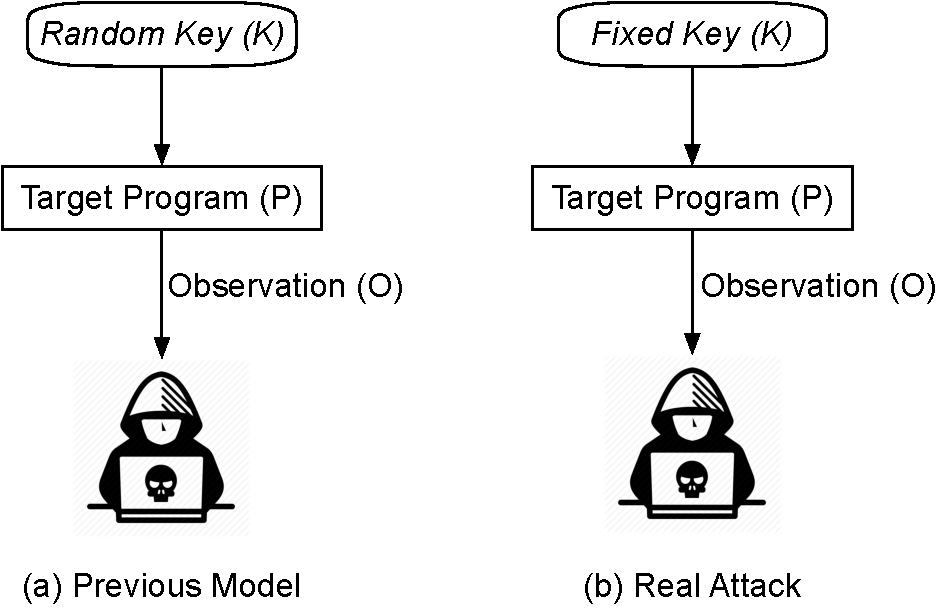
\includegraphics[width=.65\columnwidth]{./figures/RA.pdf}
\vspace*{-2pt}
    \caption{The gap between the real attack and previous models}\label{fig:gap}
    \vspace*{-5pt}
\end{figure}

Both approaches fail to tell how much information is leaked for one real execution. 
The problem with existing methods is that their approaches neglect input values and 
real runtime information. 
They assume an attacker runs the program multiple times with many different or 
random sensitive inputs. As
shown in Figure~\ref{fig:gap}(a), previous models, both Shannon entropy and max
entropy, give an ``average'' estimate of the information leakage. However, it is
not the typical scenario for an adversary to launch a side-channel attack. When
a side-channel attack happens, the adversary wants to retrieve the sensitive
information, in which case the sensitive information is fixed (e.g., AES keys).
The adversary can perform the attack over and over again with fixed input and 
guess the value bit by
bit (e.g., Kocher's timing attacks~\cite{kocher1996timing}), as in Figure~\ref{fig:gap}(b). 
We want to have a theory for dynamic analysis that if the theory says an attack leaks $x$ bits of
secret information, then $x$ should be useful in estimating the sensitive level of the vulnerability. 
However, the above methods all fail in real attack models. This is the first challenge we face
\textbf{(Challenge C1)}.

\subsection{Notations}
In the section, we give necessary definitions and notations for dealing with
programs and side-channels. We use capital letters (e.g., $A$) to represent a
set. $|A|$ represents the cardinality of the set $A$. We use corresponding lower case
letters to represent one element in the set (e.g., $a \in A$).

We assume a program ($\beta$) has $K$ as the sensitive input. $K$ should be 
a finite set of keys. The program also takes known messages $M$ as the input. 
During an AES encryption, for example, 
$\beta$ is the encryption function. $K$ is the set of all possible AES keys, 
and $ M $ is encrypted messages. In a real execution, an adversary may have 
some observations ($O$) from the program. Examples of those observations include 
timing, CPU usages, and Electromagnetic signals (EM). In this paper, 
we consider secret-dependent control-flows and secret-dependent memory 
accesses as observations.

With the above definition, we have the following mapping between $\beta$,
$K$, $M$, and $O$:
\vspace*{-5pt}
\begin{displaymath}
    \beta(K, M) \rightarrow O
\end{displaymath}


We model a side-channel in the following way. An adversary does not have
access to $K$, but he knows $\beta$, $M$, and $O$. For one execution of a
deterministic program, once $k \in K$ and $m \in M$ are fixed, the observation
($o \in O$) should also be determined. As an attacker, he knows $\beta$, $o$,
and $m$. The attacker wants to infer the value of $k$. We use $K^o$ to denote
the set of possible $k$ values that produce the same observation: $K^o = \{ k \in K \, |\, \beta(k, m) \rightarrow o\}$

Then the problem of quantifying the amount of leaked information can be
transferred into the following question.

\emph{How much uncertainty of $K$ can be reduced if an attacker knows $\beta$, $m$, and $o$?}

\subsection{Theoretical Analysis \textbf{(Solution to Challege C1)}}
In information theory, the mutual information (I) is a measure of the mutual
dependence between two variables. We use $I$ to describe the
dependence between original sensitive keys ($K$) and attackers' observations ($O$).
%which is defined as:

%\begin{equation} \label{eq:1}
%    I(K;O) = \sum_{k {\in} K}{\sum_{o {\in} O}{p(k, o)\log_2\frac{p(k, o)}{p(k)p(o)}}}
%\end{equation}

%where $P(k_i, o_i)$ is the joint discrete distribution of $K$ and $O$.
%Alternatively, the mutual information can also be equivalently expressed as:
\begin{equation} \label{eq:2}
    I(K;O) = H(K) - H(K|O)
\end{equation}

$H(K|O)$ is the entropy of $K$ under the condition $O$. It quantifies the
uncertainty of $K$, given the value of $O$. In other words, the conditional 
entropy $H(K|O)$ marks the uncertainty about $K$ after an adversary has 
gained some observations ($O$).

\begin{equation}
    H(K|O) = - \sum_{o {\in} O} {p(o) \sum_{k {\in} K}{p(k|o)\log_2p(k|o)}}
\end{equation}

In this project, we hope for a very precise definition of information
leakages. Suppose an attacker runs the target program with one
input, we want to know how much information he can infer by observing the
memory access patterns ($o$). We come to the simple slogan
~\cite{10.1007/978-3-642-00596-1_21} %% where the information
%% leakage equals:
%% \textbf{Initial uncertainty - remaining uncertainty}
that
\begin{align*}
     & \mathit{Information\ leakage} =                                         \\
     & ~~~~ \mathit{Initial\ uncertainty} - \mathit{Remaining\ uncertainty}.
\end{align*}

Next we compare the Eq.~(\ref{eq:2}) with the above slogan, we find $H(K)$
is the $\mathit{Initial\ uncertainty}$ and $H(K|O)$ is $\mathit{Remaining\
uncertainty}$. During a real attack, the observation ($o$) is known. Thus we
have $H(K|O) = H(K|o)$. Therefore, we define the amount of leaked information as

\begin{displaymath}
    Leakage = H(K;o) = H(K) - H(K|o)
\end{displaymath}

For a program ($\beta$) without any domain information, all possible sensitive
inputs should appear equally. Therefore, for any $k \in K$, $p(k) =
\frac{1}{|K|}$. We have
%\vspace*{-5pt}
$$H(K) = \sum_{k {\in} K}\frac{1}{|K|}\log_2{|K|} = \log_2{|K|}$$
%\vspace*{-5pt}

For any $k' \in K \setminus K^o$, $p(k'|o) = 0$. We get
\begin{align*}
    H(K;o) & = - \sum_{k {\in} K^o}{p(k|o)\log_2p(k|o)}                         \\
           & \qquad   - \sum_{k` {\in} (K \setminus K^o)}{p(k'|o)\log_2p(k'|o)} \\
           & = \log_2{|K^o|}
\end{align*}

\begin{mydef}
    \label{def}
    Given a program $\beta$ with the input set $K$,
    an adversary has the observation $o$ when the input $k{\in}K^o$.
    We denote it as
    $$\beta(K^o, m) \rightarrow	o$$

    The amount of leaked information $L_{\beta(k)\rightarrow o}$ based on the observation ($o$) is
    $$L_{\beta(k)\rightarrow o} = \log_2{|K|} - \log_2{|K^o|}$$
\end{mydef}
\vspace*{-5pt}

The above definition~\cite{AskarovC12} can be understood in an intuitive way. Suppose an attacker
guesses a 128-bit encryption key. 
Without any domain knowledge, 
he can find the key by performing an exhaustive search over $2^{128}$ possible keys. 
However, the program has a side-channel leakage site. After the program finishes execution, the
attacker gets some leaked information and only needs to find the key by performing an
exhaustive search over $2^{120}$ possible keys. Then we can say that 8 bits of the information
is leaked. In this example, $2^{128}$ is the size of $K$ and $2^{120}$ is the size of $K^o$.

With the definition, if an attacker observes that the code in
Figure~\ref{fig:password-checker} runs the branch 1, then the $K^{o^{1}} =
\{\mathrm{``password"}\}$. Therefore, the information leakage $L_{P(k)=o^{1}} =
\log_2{2^{64}} - \log_2{1} = 64$ bits, which means the key is totally leaked. If
the attacker observes the code hits branch 2, the leaked information is
$L_{P(k)=o^{2}} = \log_2{2^{64}} - \log_2{(2^{64}-1)} \approx 0$ bit.

As the size of input sensitive information is
usually public, the problem of quantifying the leaked information has been
transferred into the problem of estimating the size of input key $|K^o|$ under
the condition $o \in O$. 

\subsection{Our Conceptual Framework}
\label{side-channel:condition}
We now discuss how to model observations ($O$), which are the direct information
that an adversary can get during the attack.

During the execution, a program ($\beta$) have many temporary values ($t_i \in
T$). Once $\beta$ (program), $k$ (secret), and $m$ (message, public) are
determined, $t_i$ is also fixed. Therefore, $ t_i = f_i(\beta, k, m)$, where $f_
i$ is a function that maps between $t_i$ and ($\beta$, $k$, $m$).

In the paper, we consider two code patterns that can be exploited by an attacker,
\emph{secret-dependent control transfers} and \emph{secret-dependent data
accesses}. 
%In other words, an adversary has observations based on control-flows and data accesses.

\subsubsection{Secret-dependent Control Transfers}
We think a control-flow is secret-dependent if different input sensitive keys
($K$) can lead to different branch conditions. 
We define a branch is secret-dependent if:
$$\exists k_{i1}, k_{i2} \in K, \,f_i(\beta, k_{i1}, m) \neq f_i(\beta, k_{i2}, m)$$

An adversary can observe which branch the code executes, if the branch condition
equals to $t_b$. We use the constraint $c_i : f_i(\beta, k, m) = t_b$ to model
the observation ($o$) on secret-dependent control-transfers.

\subsubsection{Secret-dependent Data Accesses}
Similar to secret-dependent control-flow transfers, a data access operation is
secret-dependent if different input sensitive keys ($K$) can lead to different
memory addresses. We use the model from CacheD~\cite{203878}. The low $L$ bits
of the address are irrelevant in side-channels.

We consider a data access is secret-dependent if:
$$\exists k_{i1}, k_{i2} \in K, \,f_i(\beta, k_{i1}, m) >> L \neq f_i(\beta, k_{i2}, m) >> L$$

If the memory access equals to $t_b$, we can use the constraint $c_i :
f_i(\beta, k, m) >> L = t_b >> L$ to model the observation on secret-dependent
data accesses.

%With the above definitions, we can model an attacker's observation by a series of math
%formulas. For example, in Figure~\ref{fig:side-channel}, if an attacker observes
%the code executes the branch 1, we have $c_5: k_1 + k_2 < 4$ to describe an
%attacker's knowledge and $K^{o5} = \{k_1,\, k_2\,|\, (k_1 + k_2) < 4\}$. If an
%attacker observes the code executes the branch 2, we have $c_8: k_1 - k_2 > 0$
%and $K^{o8} = \{k_1,\, k_2\,|\, (k_1 - k_2) > 0\}$.

\section{Scalable to Real-world Crypto Systems}
\label{sec:scala}

In \S\ref{sec:trace-qif}, we propose an advanced information leakage definition for
realistic attack scenarios to model two types of address-based side-channel
leakages as math formulas, and quantify them by calculating the number of input
keys ($K^o$) that satisfy those math formulas. Intuitively, we can use
traditional symbolic execution to capture math formulas and model counting
to get the number of satisfying input keys ($K^o$). However, some preliminary
experiments show that the above approach suffers from unbearable costs, which
impede its usage to detect and quantify side-channel leakages in real-world
applications. In this section, we begin by discussing the bottlenecks of
applying the above approaches in real-world software. After that, we
propose our methods.

In general, \tool{} faces the following performance challenges in
order to \emph{scale to production crypto system analysis}.
\begin{itemize}
      \item Symbolic execution (\textbf{Challenge C2})
      \item Counting the number of items in $K^o$ (\textbf{Challenge C3})
\end{itemize}

\subsection{Trace-oriented Symbolic Execution}
Symbolic execution is notorious for its unbearable performance cost. 
Previous trace-oriented
symbolic execution based
works~\cite{203878,Chattopadhyay:2017:QIL:3127041.3127044} have large
performance bottlenecks. As a result, those approaches either only apply to
small-size programs~\cite{Chattopadhyay:2017:QIL:3127041.3127044} or apply some
domain knowledge~\cite{Wang:2007:NCD:1250662.1250723} to simplify the analysis. 
%Those tools interpret each
%instruction and update memory cells and registers with formulas that
%captured the semantics of the execution and search different input values that
%can lead to different execution behaviors using constraint solver. 
We implement
the approach presented in \S\ref{sec:trace-qif} and model the side-channels as
formulas. While the tool can finish analyzing some simple cases like AES, it can
not handle complicated cases like RSA.
We observe that finding side-channels using symbolic execution is different from
traditional general symbolic execution and can be optimized to be as efficient
as other methods with approaches below.

\subsubsection{Interprete Instructions Symbolically}
Existing binary analysis tools~\cite{shoshitaishvili2016state,
10.1007/978-3-642-22110-1_37} translate machine instructions into
intermediate languages (IR) to simplify the analysis. 
The reason is that the number of machine instructions is
enormous, and the semantics of each instruction is complex. Intel Developer
Manual~\cite{intelsys} introduces more than 1000 different x86 instructions. 
However, the IR layer, which predigests the implementation
and reduces the workload of those tools, is not suitable for side-channels 
analysis.
In general, IR-based or source code side-channels analyses are not accurate enough.
In many cases, compilers use conditional moves or bitwise operations to eliminate
branches. Also, as some IRs are not a superset or a subset of ISA, 
it is hard to rule out conditional jumps introduced by IR and add real branches 
eliminated by IR transformations.

Moreover, the IR design causes significant overhead~\cite{217563}.
Transferring machine instructions into IR is time-consuming. For example,
REIL IR~\cite{dullien2009reil}, adopted in CacheS~\cite{236338}, has multiple
transform processes, from binary to VEX IR, BAP IR, and finally REIL IR\@. 
Also, IR increases the total number of instructions. For example, x86
instruction \textit{test eax, eax} transfers into 18 REIL IR instructions. 

%\vspace*{2pt}
\textbf{Our Solution:}
We abandon the IR design and take the engineer efforts to implement 
the symbolic execution directly on the top of x86 instructions from scratch. 
Table~\ref{scala:ir} shows that eliminating the IR layer can reduce the number 
of instructions executed during the analysis. Previous works~\cite{217563} also 
has a similar approach to speed up the fuzzing. Our implementation is different
from their works in two aspects: 1) We use complete constraints. 2) We run the
symbolic execution on one execution path each time. Our result indicate the 
design is around 30 times faster than the IR design (transferring ISA into IR and
symbolically executing instructions).

\begin{table}%[ht]
      \centering\small\footnotesize
      \caption{The number of x86,  % instructions and the number of 
             REIL IR, and VEX IR instructions on the traces of crypto programs.}
      \label{scala:ir}
\vspace*{-5pt}
      \resizebox{\columnwidth}{!}{%

            \begin{tabular}{cccc}
                  \hline
                                    & \begin{tabular}[c]{@{}c@{}}Number of\\ x86 Instructions\end{tabular} & \begin{tabular}[c]{@{}c@{}}Number of\\ VEX IR\end{tabular} & \begin{tabular}[c]{@{}c@{}}Number of\\ REIL IR\end{tabular} \\ \hline
                  AES OpenSSL 0.9.7 & $1,704$                   & $23,938$ (15x)            & $62,045$ (36x)            \\
                  DES OpenSSL 0.9.7 & $2,976$                   & $41,897$ (15x)            & $100,365$ (33x)           \\
                  RSA OpenSSL 0.9.7 & $1.6*10^7$                & $2.4*10^8$ (15x)          & $5.9*10^8$ (37x)          \\
                  RSA mbedTLS 2.5  & $2.2*10^7$                & $3.1*10^8$ (15x)          & $8.6*10^8$  (39x)         \\ \hline
            \end{tabular}
      }
      \vspace*{-16pt}
\end{table}

\subsubsection{Constraint Solving}
As discussed in \S\ref{side-channel:condition}, the problem of identifying
side-channels can be reduced to the question below.

\begin{quote}
      \textit{Can we find two different input variables $k_1, k_2 \in K$ that
            satisfy the formula $f_a(k_1) \neq f_a(k_2)$?}
\end{quote}

Existing approach relies on satisfiability modulo theories (SMT) solvers 
(e.g, Z3~\cite{DeMoura:2008:ZES:1792734.1792766}) to find satisfying 
$k_1$ and $k_2$.
We argue that while it is a universal approach to solving constraints 
with SMT solvers, for constraints with the above formats, using custom 
heuristics and testing is much more efficient in practice. Constraint 
solving is a decision problem expressed in logic formulas. SMT solvers 
transfer the inputted SMT formula into the boolean conjunctive normal 
form (CNF) and feed it into the internal boolean satisfiability 
problem (SAT) solver. The translation process, called ``bit blasting'', 
is time-consuming. Also, as the SAT problem is a well-known NP-complete 
problem, it is hard to deal when it comes to
practical uses with huge formulas. Despite the rapid development 
of SMT solvers in recent years, constraint solving remains one of 
the obstacles to achieving the scalability of analyzing real-world cryptosystems.

%\vspace*{2pt}
\textbf{Our Solution:}
Instead of feeding the formula $f_a(k_1) \neq f_a(k_2)$ into a SMT solver, we
randomly pick up $k_1, k_2 \in K$ and test them if they can satisfy the
formula. Our solution is based on the following intuition. For most combination
of $(k_{1}, k_{2} )$, the formula $f_a(k_1) \neq f_a(k_2)$ holds. As long as
$f_a$ is not a constant function, such $k_1, k_2$ must exist. For example,
suppose each time we only have 5\% chance to find such $k_1, k_2$, then after we
test with different input combination with 100 times, we have $1 -
(1-0.05)^{100} = 99.6\%$ chance find such $k_1, k_2$. Such random algorithms
work well for our problem.

\subsection{Counting the Number}
\label{MCreasons}
%According to
%Definition~\ref{def} introduced in \S\ref{sec:trace-qif},
%the problem of quantifying the amount of leaked information can be reduced to
%the problem of computing the number of items in $K^o$. However, we find that while
%there are various propositional model counters (e.g., \#SAT), they are not
%sufficient scalable for production cryptosystem analysis.
%there is no open source modulo theories counter (\#SMT) available.

%One straightforward method approximating the number of solutions is based on Monte Carlo
%sampling. However, the number of satisfying values could be exponentially small.
%Consider the formula $f_i\equiv{k_1} = 1\land{k_2} = 2\land{k_3} = 3\land{k_4} =
%4$, where $k_1$, $k_2$, $k_3$, and $k_4$ each represents one byte in the
%original sensitive input buffer, there is only one satisfying solution of total
%$2^{32}$ possible values, which requires exponentially many samples to get a
%tight bound. Monte Carlo method also suffers from the curse of dimensionality.
%For example, the length of an RSA private key can be as long as 4096 bits. If we
%take each byte (8 bits) in the original buffer as one symbol, the formula can
%have as many as 512 symbols.

%\vspace*{2pt}
%\textbf{Our Solution to Challenge C3:}
%We adopt multiple-step Monte Carlo sampling methods to count the number of
%possible inputs that satisfy the logic formula groups. The key idea is to split
%those constraints into several small formulas and sample them independently.
%We will introduce the method in the following subsection.

%\subsection{Information Leakage Estimation}

\newcommand{\addr}[1]{{l}_{#1}}
\renewcommand{\addr}[1]{{\gamma}_{#1}}
\renewcommand{\addr}[1]{{\zeta}_{#1}}
\renewcommand{\addr}[1]{{\xi}_{#1}}

In this section, we present the algorithm to calculate the information leakage
based on Definition~\ref{def} (\S\ref{sec:trace-qif}), answering to
\textbf{Challenge C3}.

\subsubsection{Problem Statement}
For each leakage site, we model it with a math formula constraint with the
method presented in~\S\ref{side-channel:condition}. Suppose the address of the
leakage site is $\addr{i}$, we use $c_{\addr{i}}$ to denote the constraint
that models the side-channel leakage. 
%For
%multiple leakage sites, we take the conjunction of those constraints to
%represent those leakage sites.

According to the Definition~\ref{def}, to calculate the amount of leaked
information, the key is to calculate the cardinality
of $K^o$. Suppose an attacker can observe $n$ leakage sites, and each leakage
site has the following constraints: $c_{\addr{1}}, c_{\addr{2}}, \ldots,
c_{\addr{n}}$ respectively. The total leakage can be calculated from the constraint
$c_t({\addr{1}},{\addr{2}},\ldots,{\addr{n}}) = c_{\addr{1}} \land c_{\addr{2}}
\land \ldots \land c_{\addr{n}}$. 
%%The problem of estimating the total leaked
%%information can be reduced to the problem of counting the number of different
%%solutions that satisfies the constraint
%%$c_t({\addr{1}},{\addr{2}},\ldots,{\addr{n}})$. 
A simple method is to pick elements $k$ from $K$ and check if the
element also contained in $K^o$. Assume $q$ elements satisfy this condition. In
expectation, we can use $\frac{k}{q}$ to approximate the value of
$\frac{|K|}{|K^o|}$.

However, the above sampling method fails in practice due to the following two problems:

\begin{enumerate}
      \item The curse of dimensionality problem. $c_t({\addr{1}},\ldots,{\addr{n}})$ is
            the conjunction of many constraints. Therefore, the input variables
            of each constraints will also be the input variables of the
            $c_t({\addr{1}},\ldots,{\addr{n}})$. The sampling method will fail
            as $n$ increases. 

            %For example, if the program has $2$ input whose size is 
            %one byte, the whole search space is a $256^2$ cube. If we want
            %the sampling distance between each point equals to $d$, we need
            %$256^2d$ points. If the program has $10$ byte input, we need
            %$256^{10}d$ points if we still we want the sampling distance equals
            %to $d$.

      \item The number of satisfying assignments could be exponentially small.
            According to Chernoff bound, we need exponentially many samples to
            get a tight bound. 
            %On an extreme situation, if the constraint only
            %has one unique satisfying solution, the simple Monte Carlo method
            %cannot find the satisfying assignment even after sampling many
            %points.
\end{enumerate}

However, despite above two problems, we also observe two characteristics of the
problem:
\begin{enumerate}
      \item $c_t({\addr{1}},{\addr{2}},\ldots,{\addr{n}})$ is the conjunction of
            several short constraints $c_{\addr{i}}$. The set containing the
            input variables of $c_{\addr{i}}$ is the subset of the input
            variables of $c_t({\addr{1}},{\addr{2}},\ldots,{\addr{n}})$. Some
            constraints have completely different input variables from other
            constraints.

            \item Each time when we sample $c_t({\addr{1}},{\addr{2}},\ldots,{\addr{n}})$
            with a point, the sampling result is \emph{Satisfied} or not \emph{Not Satisfied}.
            The result is randomly generated in a way that does not depend on the result in 
            previous experiments. Also, as the amount of leaked information is calculated
            by $\log$ function, we do not need to count the number of solutions for 
            a given constraint precisely.
            %\item For each constraint $F(C_{{addr}_i})$, the satisfying assignments
            %are close to each other, which means if we find one satisfying assignment, we 
            %are more likely to find other satisfying assignments nearby than randomly
            %pick one point in the whole searching space.

\end{enumerate}

In regard to the above problems, we present our methods. First, we split
$c_t(\addr{1},\addr{2},\ldots,\addr{n})$ into several independent constraint
groups. After that, we run a multi-step sampling method for each constraint.

\subsubsection{Maximum Independent Partition}

For a constraint $c_{\addr{i}}$, we define function $\pi$, which maps the
constraint into a set of different input symbols. For example, $\pi(k1 + k2 >
128) = \{k1, k2\}$.

\begin{mydef}[]
      \label{independentC}
      Given two constraints $c_m$ and $c_n$, we call them independent iff
      $$\pi(c_m) \cap \pi(c_n) = \emptyset$$
\end{mydef}

Based on the Definition~\ref{independentC}, we can split the constraint
$c_t(\addr{1},\addr{2},\ldots,\addr{n})$ into several independent constraints.
There are many partitions. For our project, we are interested in the following
one.

\begin{mydef}\label{Goodpartition}
      For the constraint $c_t(\addr{1},\addr{2},\ldots,\addr{n})$,
      we call the constraint group
      $g_{1}, g_{2}, \ldots, g_{m}$
      the maximum independent partition of $c_t(\addr{1},\addr{2},\ldots,\addr{n})$ iff
      \begin{enumerate}
            \item $g_{1} \land g_{2} \land \ldots \land g_{m} = c_t(\addr{1},\addr{2},\ldots,\addr{n})$
            \item $\forall i, j \in \{1, \ldots, m\} \quad \textrm{and} \quad
                        i \neq j,\quad\pi(g_{i}) \cap \pi(g_{j}) = \emptyset $
            \item For any other partitions  $h_{1}, h_{2}, \ldots, h_{m'}$ satisfy 1) and
                  2), $m \geq m'$
      \end{enumerate}

\end{mydef}

The reason we want a good partition of constraints is we want to reduce
the dimensions. For example,
A good partition of $F: ({k_1} = 1)\land({k_2} = 2)\land({k_3} > 4)\land({k_3} - {k_4} > 10)$ would be
$g_{1}: ({k_1} = 1)\quad g_{2}: ({k_2} = 2)\quad g_{3}: ({k_3} > 4) \land
({k_3} - {k_4} > 10)$  
We can sample each constraint independently and combine them together
with Theorem~\ref{IndependentConstraint}.

\begin{theorem}
      \label{IndependentConstraint}
      Let $g_{1}, g_{2}, \ldots, g_{m}$ be a maximum independent partition of
      $c_t(\addr{1},\addr{2},\ldots,\addr{n})$.
      $K_c$ is the input set that satisfies constraint $c$. We can have the following
      equation in regard to the size of $K_c$
      $$|K_{c_t(\addr{1},\addr{2},\ldots,\addr{n})}| = |K_{g_{1}}|*|K_{g_{2}}|*\ldots*|K_{g_{n}}|$$
\end{theorem}
\vspace{-3pt}
With Theorem~\ref{IndependentConstraint}, we transfer the problem of
counting the number of solutions to a complicated constraint in high-dimension
space into counting solutions to several small constraints. We compute the
maximum independent partition by iterating each $\addr{i}$ and applying the function
$\pi$ over the constraint $\addr{i}$.

%% We apply the following
%% algorithm~\ref{algo:max-inde} to get the Maximum Independent Partition of the
%% $c_t(\addr{1},\addr{2},\ldots,\addr{n})$.

%% \IncMargin{1em}
%% \begin{algorithm}[h]
%%       \DontPrintSemicolon
%%       \SetKwInOut{Input}{input}\SetKwInOut{Output}{output}
%%       \Input{$c_t(\addr{1},\addr{2},\ldots,\addr{n}) = c_{\addr{1}} \land c_{\addr{2}} \land \ldots \land c_{\addr{m}}$}
%%       \Output{The Maximum Independent Partition of $G = \{g_{1}, g_{2}  , \ldots,  g_{m} \}$ }
%%       \For{$i\leftarrow 1$ \KwTo $n$}
%%       {
%%             $S_{c_i}$ $\leftarrow$ $\pi(c_{\addr{i}})$ \;
%%             \For{$g_{i} \in G$}
%%             {
%%                   $S_{g_i}$ $\leftarrow$ $\pi(g_{i})$ \;
%%                   $S$ $\leftarrow$ $S_{C_i} \cap S_{G_i}$  \;
%%                   \If{$S \neq \emptyset$}
%%                   {
%%                         $g_{i} \leftarrow g_{i} \land g_{\addr{i}}$ \;
%%                         \textbf{break} \;
%%                   }
%%                   Insert $c_{\addr{i}}$ to $G$
%%             }
%%       }
%%       \caption{The Maximum Independent Partition}
%%       \label{algo:max-inde}
%% \end{algorithm}
%% \DecMargin{1em}

\subsubsection{Multiple Step Monte Carlo Sampling}

After we split those constraints into several small constraints, we count the
number of solutions for each constraint. Even though the dimension has been
significantly reduced after the previous step, this is still a \#P problem. 
%For our
%project, we apply the approximate counting instead of exact counting for two
%reasons. First, we do not need to have a very precise result of the exact number
%of total solutions since the information is defined with a logarithmic function.
%We do not need to distinguish between constraints having $10^{10}$ or $10^{10} +
%10$ solutions; they are very close to after taking logarithmic. Second, the
%precise model counting approaches, like Davis-Putnam-Logemann-Loveland (DPLL)
%search, have difficulty scaling up to large problem sizes.

We apply the ``counting by sampling'' method. For
the constraint $g_{i}= c_{i_1} \land c_{i_2} \land ,\ldots, \land c_{i_j} \land
,\ldots, \land c_{i_m}$, if the solution satisfies $g_{i}$, it should also
satisfy any constraint from $c_{i_1}$ to $c_{i_m}$. In other words, $K_{c_gi}$
should be the subset of $K_{c_1}$, $K_{c_2}$, \ldots , $K_{c_m}$. We notice that
$c_i$ usually has less numbers of input compared to $g_{i}$. For example, if
$c_{i_j}$ has only one 8-bit input variable, we can find the exact solution set
$K_{c_{i_j}}$ of $c_{i_j}$ by trying every possible 256 solutions. After that,
we can only generate random input numbers for the rest input variables in
constraint $g_{i}$. With this simple yet effective trick, we can reduce the number of input
while still ensure the accuracy.

%% the algorithm
%\IncMargin{1em}
%\begin{algorithm}
%\SetAlgoLined
%\DontPrintSemicolon

%\KwIn{{The constraint $G_{i}= C_{i_1} \land C_{i_2}
%\land \ldots \land C_{i_m}$}}    
%\KwOut{{The number of assignments that satisfy $G_{i}$ $|K_{G_{i}}|$}}

%\SetKwProg{RW}{RandomWalk}{}{}
%\SetKwProg{MM}{MetropolisMove}{}{} 
%$n$: the number of sampling times \;
%$P$: a probability generator \;
%$k$: the input assignment \;
%$n_{s}$: the number of satisfying assignments \;
%$\#k$: the satisfying number of k \fixme{this number is not used syntactically} \; 
%Initialization: \;
%$\#{k_0}$ $\leftarrow$ $\sum_{j=1}^{m}C_{i_j}(k_0)$ \;
%\For{$t\leftarrow 1$ \KwTo $n$} {
%      $p$ $\leftarrow$ $P$ \;
%      \If{$p \geq 0.5$}
%      {
%        $v$ $\leftarrow$ \RW{$v$} {}
%      }
%      \Else{
%            $v$ $\leftarrow$ \MM{$v$} {}
%      }
%      \If{$v$ satisfies $G_{i}$}
%      {$n_{s}$ $\leftarrow$ $n_{s} + 1$}
%}
%$|K_{G_{i}}|$ $\leftarrow$ $n_s|K| / n$
%\caption{Metropolis Sampling}
%\end{algorithm}
%\DecMargin{1em}

\subsubsection{Error Estimation}
\label{sssec:errest}
Our result has the probabilistic guarantee that the error of the estimated amount of leaked 
information is less than 1 bit under the Central Limit Theorem (CLT) and uncertainty
propagation theorem.

Let $n$ be the number of samples and $n_s$ be the number of samples that satisfy
the constraint $C$. Then we can get $\hat{p} = \frac{n_s}{n}$. If we repeat the
experiment multiple times, each time we can get a $\hat{p}$. As each
$\hat{p}$ is independent and identically distributed, according to the central limit
theorem, the mean value should follow normal distribution
$ \frac{\bar{p}-E(p)}{\sigma\sqrt{n}} \rightarrow N(0,1) $. Here $E(p)$ is the
mean value of $p$, and $\sigma$ is the standard variance of $p$. If we use the
observed value $\hat{p}$ to the calculate the standard deviation, we can claim that
we have 95\%\footnote{For a normal distribution, 95\% of variable $\Delta p$ fall within two sigmas of the mean.} 
confidence that the error $\Delta p= \bar{p} - E(p)$ falls in the interval:
$$ |\Delta p| \leq 1.96\sqrt{\frac{ \hat{p} (1- \hat{p} )}{n}}$$

Since we use $L = \log_{2}p$ to estimate the amount of leaked information, we
can have the following error propagation formula $\Delta L = \frac{\Delta
p}{p\ln2}$ by taking the derivative from Definition~\ref{def}. For \tool, we want the error of estimated leaked
information ($\Delta L$) to be less than 1 bit. So we get $\frac{\Delta
p}{p\ln2} \leq 1$. Therefore, as long as $ n \geq \frac{1.96^2(1-p)}{p(\ln2)^2}$, we can have
95\% confidence that the error of estimated leaked information is less than 1 bit.
During the simulation, if $n$ and $p$ satisfy the above inequation, Monte Carlo
simulation will terminate.

%\section{Design}
\section{Design and Implementation}
In this section, we describe the design of \tool{} by focusing on how our design
solves the challenges discussed in the previous section.

%\subsection{Overview}
%\subsection{Workflow}
\subsection{Design}
The shortcomings of the existing work inspire us to design a new tool to detect
and quantify side-channel vulnerabilities in binaries. The tool has three steps,
as shown in Figure~\ref{fig:workflow}. First, we run the target program with a
concrete input (sensitive information) under the dynamic binary instrumentation
(DBI) frameworks to collect execution traces. After that, we run the symbolic
execution to capture the fine-grained semantic information of each
secret-dependent control-flow transfers and data-accesses. Finally, we run Monte
Carlo (MC) simulations to estimate the amount of leaked information.

\begin{figure*}[t]
    \centering
    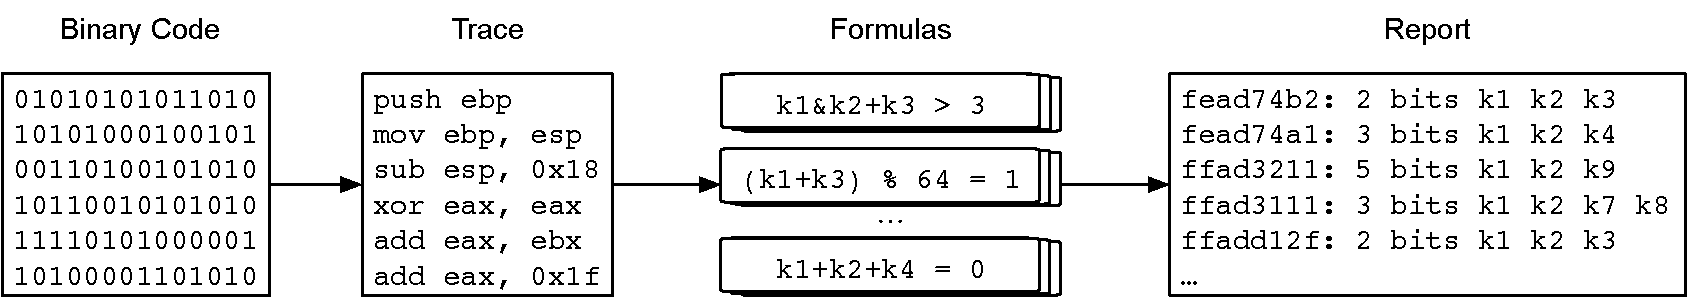
\includegraphics[width=0.8\textwidth]{./figures/workflow.pdf}
    \caption{The workflow of \tool{}.}
    \label{fig:workflow}
\end{figure*}

\begin{enumerate}
    \item \emph{Execution trace generation.} The design goal of \tool{} is to
          estimate the information leakage as precisely as possible. Therefore,
          we sacrifice the soundness for precision in terms of program
          analysis. We run the target binary under dynamic binary instrumentations (DBI) to
          record execution traces and the runtime information.
    \item \emph{Instruction level symbolic execution.} We model attackers'
          observations from side-channel vulnerabilities with logic formulas.
          Each formula captures the fined-grained information between input
          secrets and leakage sites. In consideration of precision and
          performance, we remove the intermediate language(IR) layer of the
          symbolic execution. Also, the engine only symbolically executes the
          instruction that might be affected by the input key. We use random
          testing instead of SMT solvers to find satisfying variables. 
    \item \emph{Leakage estimation.} We transfer the information leakage quantification
          problem into the problem of counting the number of assignments that satisfy the
          formulas which model the observations from attackers. We propose a
          Monte Carlo method to estimate the number of satisfying solutions.
          With the help of the central
          limit theorems (CLT), we also give an error estimate with the probability,
          which gives us the \emph{precision guarantee}.

\end{enumerate}


%% \subsection{Trace Logging}
%% The trace information can be logged via some emulators (e.g., QEMU) or 
%% dynamic binary instrumentation tools (DBI). 
%% We run a program with the concrete input under the DBI to record
%% execution traces.
%% The trace data has the following information:
%% \begin{itemize}
%%     \item Each instruction mnemonics and its memory address.
%%     \item The operands of each instruction and their concrete values during the 
%%           runtime.
%%     \item The value of EFLAGS register. 
%%     \item The memory address and the length of the sensitive information.
%%      Most crypto libraries stores sensitive information in arrays,
%%      variables or contiguous buffer.
%% \end{itemize}

%% \subsection{Instruction Level Symbolic Execution}
%% \label{InstructionSE}
%% The primary purpose of the step is to generate constraints of the input 
%% sensitive information from the execution trace. 
%% If we give the target program a new input which 
%% is different from the original input that was used 
%% to generate the execution trace but still satisfies those constraints,
%% as an attacker, he will have the same observations on
%% control-flow transfer and 
%% data-access patterns.

%% The tool runs symbolic execution on top of execution traces.
%% At the beginning of the symbolic execution, the tool creates new 
%% symbols for each byte in the raw buffer. For other data in the 
%% register or memory at the beginning, we use actual values from the 
%% runtime information collected during the runtime. 
%% During the symbolic execution for each instruction, 
%% the tool updates every variable in the memory and registers with a
%% math formula. The formula is made up of concrete values and the input 
%% key as the symbols accumulated through the symbolic execution.
%% For each formula, the tool will check weather it can be reduced
%% into a concrete values (e.g., $k_1+12-k_1 = 12$ ). 
%% If so, the tool will only use the concrete values in the 
%% following symbolic execution.

%% \subsubsection{Verification and Optimization}
%% We run the symbolic execution (SE) on top of x86 instructions.
%% In other words, we do not rely on any intermediate languages to simplify the implementation of symbolic execution. 
%% While the implementation itself has a lot of benefits (Better performance, accurate memory model), 
%% we need to implement the symbolic execution rules for each x86 instruction. 
%% However, due to the complexity of x86, it is inevitable to make mistakes. 
%% Therefore, we verify the correctness of the SE engine during the execution. 
%% The tool will collect the runtime information (Register values, 
%% memory values) and compare them with the formula generated from the symbolic execution. Whenever the tool finishes the symbolic execution of each instruction, the tool will compare the formula for each symbol and its actual value. If the two values do not match, we check the code
%% and fix the error. Also, if the formula does not contain any symbols,
%% the tool will use the concrete value instead of symbolic execution.

%% \subsubsection{Secret-dependent control-flows}
%% An adversary can infer sensitive information from secret dependent control-flows. 
%% There are two kinds of control-transfer instructions: the unconditional 
%% control-transfer instructions and the conditional transfer instructions.
%% The unconditional instructions, like CALL, JUMP, RET transfer control
%% from one code segment location to another. Since the transfer is independent of the input sensitive information, an attacker was not able to infer any sensitive information from the control-flow. 
%% So the unconditional control-transfer does not leak any information based on our threat model. During the symbolic execution, 
%% we update the register information and memory cells with new formulas accordingly.

%% The conditional control-flow transfer instructions, like conditional jumps,
%% depending on CPU states, may or may not transfer control flows.
%% For conditional jumps, the CPU will test if certain condition flag 
%% (e.g., CF = 0, ZF =1) is met and jump to certain branches, respectively.
%% The symbolic engine will compute the flag and represent the flag in a symbol 
%% formula. Because we are running on a symbolic execution on an execution trace, 
%% we know which branch is executed.
%% If a conditional jump uses the CPU status flag, we will generate the constraint 
%% accordingly.


%% %\begin{figure}[ht]
%% %      \centering
%% %      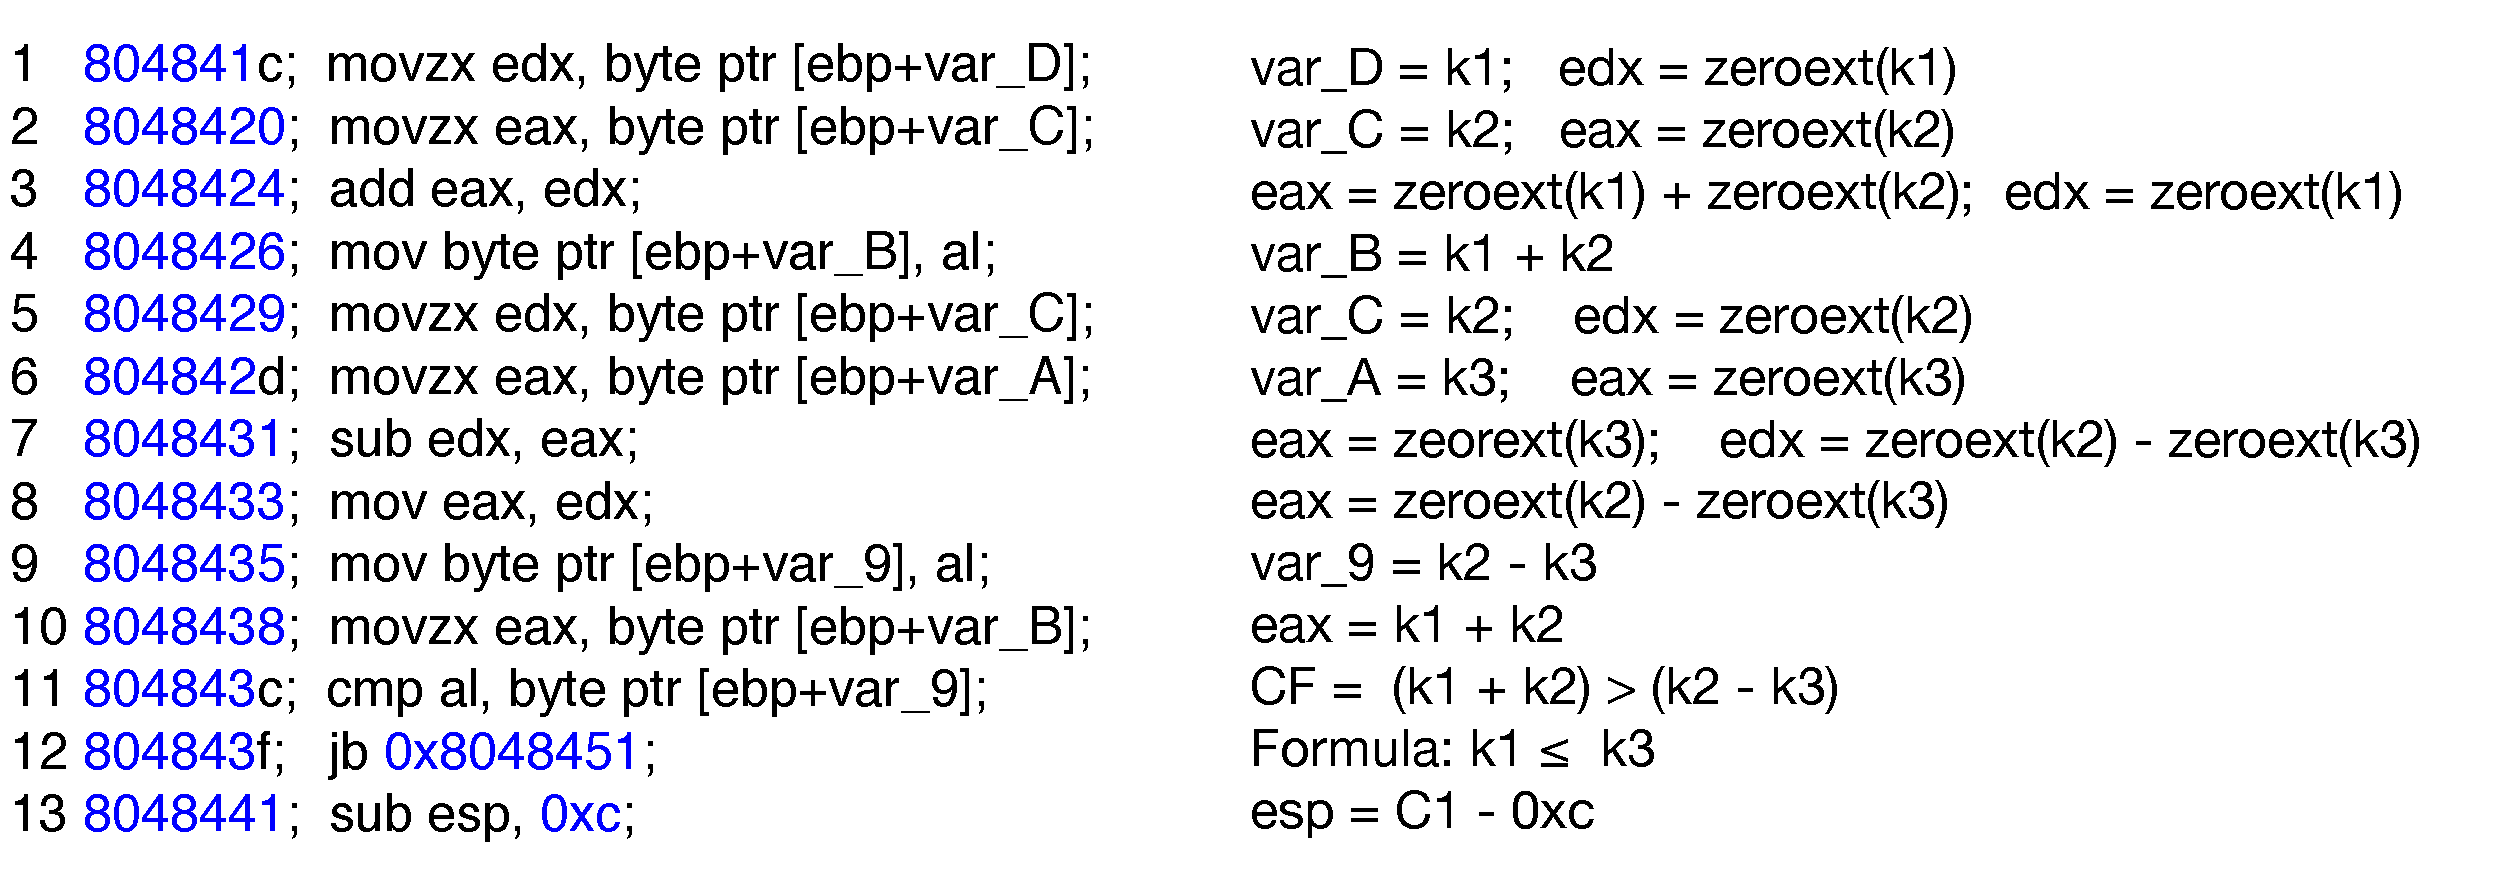
\includegraphics[width=\columnwidth]{./figures/secretCF.pdf}
%% %      \caption{The workflow of \tool{}. \fixme{fix the caption, fix the drawing.} \fixme{duplicate label.}}
%% %      \label{fig:Test-------------------}
%% %  \end{figure}

%% For examples,

%% \begin{lstlisting}
%% ...
%% 0x0000e781      add dword [local_14h], 1
%% 0x0000e785      cmp dword [local_14h], 4
%% 0x0000e789      jne 0xe7df
%% 0x0000e78b      mov dword [local_14h], 0
%% ...
%% \end{lstlisting}

%% At the beginning of the instruction segment, the value at the 
%% address of local\_14h can be written as $F(\vec{K})$. At the address $e785$, 
%% the value will be updated with $F(\vec{K})+1$. Then the code compares 
%% the value with 4 and use the result as a conditional jump. 
%% Based on the result, we can have the following formula:

%% $$F(\vec{K}) + 1 = 4$$

%% The formula, together with the memory address (0xe789) is store
%% as a \textit{formula tuple (address, formula)}. 
%% Each formula tuple represents one leakage site.

%% \subsubsection{Secret-dependent data access}
%% Like input-dependent control-flow transfers, an adversary can also infer 
%% sensitive information from the data access pattern as well. 
%% We try to find this kind of leakages by checking 
%% every memory operand of the instruction. We generate the memory addressing 
%% formulas. As discussed before, every symbols in the formula is the input key. 
%% If the formula does not contain any symbols, the memory access is independent 
%% from the input sensitive information and will not leak any sensitive information 
%% according to our threat model. Otherwise, we will generate the constraint for
%% the memory addressing. We model the memory address with a symbolic formula 
%% $F(\vec{K})$. 
%% Because we also have the concrete value of the memory address $Addr1$. 
%% Inspired by the work from~\cite{203878}, the formula can be written as:
%% $F(\vec{K}) >> L = Addr1 >> L$

%% $L$ represents the minimum memory address granularity that an attacker 
%% can observe. For example, Flush and Reload can distinguish between different
%% cache lines, which means the value of L is 6.

%% \subsubsection{Information Flow Check}
%% \tool{} is designed to help software developers find and understand the 
%% side-channel vulnerabilities. To ease the procedure of fixing the bug,
%% we also track the information flow for each byte of the input
%% buffer. 
%% The step can be seen as the multiple-tag taint analysis.
%% With the help of the information from symbolic execution, we can implement 
%% a relatively simple but relatively precise information flow track.
%% At the beginning of the analysis, \tool{} keep a track for each byte in 
%% the original buffer. When \tool{} symbolically executes each
%% instruction in the trace, it will check every value read from
%% registers or memory. If the value is concrete, it means the
%% instruction has nothing to do with the original buffer.
%% If the value is a formula, it means the original information passes through 
%% the instruction. Since each byte in the sensitive
%% buffer is represented as a symbol with a unique ID, \tool{} can
%% know which byte in the origin buffer goes through the
%% instruction.



\subsection{Implementation}
\tool{} consists of 16,729 lines of code in C++17 and Python. It has three
components: an Intel Pin tool that collects the execution trace, the
instruction-level symbolic execution engine, and the backend that estimates
the information leakage. 
%\label{appendix:code}
%\begin{table}[h!]
%    \centering
    %    \resizebox{.8\columnwidth}{!}{
%    \caption{\tool{}' main components and sizes}\label{tbl:implementation}
%    \begin{tabular}{lr@{~}@{}l}
%        \hline
%        Component            & \multicolumn{2}{c}{Lines of Code (LOC)}             \\ \hline
%        Trace Logging        & 501 lines                               & of C++    \\
%        Symbolic Execution   & 14,963 lines                            & of C++    \\
%        Data Flow            & 451 lines                               & of C++    \\
%        Monte Carlo Sampling & 603 lines                               & of C++    \\
%        Others               & 211 lines                               & of Python \\ \hline
%        Total                & 16,729 lines                            &           \\\hline
%    \end{tabular}
%    %    }
%\end{table}

Our current implementation supports most Intel 32-bit instructions that are essential to find memory-based side-channel
vulnerabilities, including bitwise operations, control transfer, data movement, and logic
instructions. The tool uses the real values to update the registers and memory for instructions that the implementation does not support. 
Therefore, the tool may miss some leakages but will not raise false positives. 

\section{Evaluation}
\label{res_overview}

\begin{table}[]
    \centering\small\footnotesize
    \caption{Evaluation results overview: Name, Side-channel Leaks\,(Leaks), 
        Secret-dependent Control-flows\,(CF), Secret-dependent Data-flows\,(DF),
        The number of instructions\,(\# Instructions), Symbolic Execution\,(SE) and Monte Carlo\,(MC) time.
    }\label{table:over_result}
    \vspace*{-5pt}
    \newlength{\x}
    \newlength{\y}
    \settowidth{\x}{~~}
    \settowidth{\y}{m}
    \addtolength{\x}{-1\y}
    \newcommand{\foo}{\mbox{\hspace*{\the\x}}}
%    \resizebox{1.9\columnwidth}{!}{
    \begin{threeparttable}
    \begin{tabular}{l@{}r@{~~}rrr@{~~}rr}
        \hline
        \textbf{Name}   & \textbf{\# Leaks} & \textbf{\# CF}         & \textbf{\# DF}
                           & \textbf{\# Instructions}    & \textbf{SE} & \textbf{MC}                                                    \\\hline
                                                 &                        &                     &                      &              & ms        & ms              \\\cline{6-7}
        AES\tnote{1}               & 68                     & 0                   & 68                   & 39,855        & 512     & 1,052         \\
        AES\tnote{2}                & 68                     & 0                   & 68                   & 39,855       & 520    & 1,057         \\
        AES\tnote{4}                & 75                     & 0                   & 75                   & 1,704        & 231    & 9,199        \\
        AES\tnote{5}                & 88                     & 0                   & 88                   & 1,350        & 36      & 1,924         \\
        AES\tnote{6}                & 88                     & 0                   & 88                   & 1,350        & 35      & 1,961        \\
        AES\tnote{7}                & 88                     & 0                   & 88                   & 1,420        & 36     & 2,161        \\
        AES\tnote{8}                & 88                     & 0                   & 88                   & 1,586        & 43      & 1,631        \\
        DES\tnote{1}                & 15                     & 0                   & 15                   & 4,596        & 58      & 162          \\
        DES\tnote{2}                & 15                     & 0                   & 15                   & 4,596        & 57      & 162           \\
        DES\tnote{4}                & 6                      & 0                   & 6                    & 2,976         & 163    & 4,677         \\
        DES\tnote{5}                & 8                      & 0                   & 8                    & 2,593         & 166    & 6,509        \\
        DES\tnote{6}                & 8                      & 0                   & 8                    & 2,593        & 165    & 5,975        \\
        DES\tnote{7}                & 8                      & 0                   & 8                    & 4,260         & 182    & 5,292        \\
        DES\tnote{8}                & 6                      & 0                   & 6                    & 8,272         & 229     & 5,152      \\
                           &                        &                     &                      &                  & seconds   & seconds               \\\cline{6-7}
        Chacha20\tnote{3}           & 0                      & 0                   & 0                    & 149,353        & 2     & 0             \\  
        Poly1305\tnote{3}           & 0                      & 0                   & 0                    & 1,213,937      & 15    & 0             \\
        Argon2i\tnote{3}            & 0                      & 0                   & 0                    & 4,595,142       & 37    & 0             \\
        Ed25519\tnote{3}            & 0                      & 0                   & 0                    & 5,713,619       & 271   & 0            \\
        ECDSA\tnote{2}              & 6                      &    6                & 0                    &  4,214,946     &  48   &   31       \\ 
        ECDSA\tnote{3}              &   4                   &   4                 & 0                    &  4,192,558    & 102   & 1639          \\   
        ECDSA\tnote{4}              &  5                    & 4                   & 1                    &  8,248,322       & 101     & 62           \\   
        ECDSA\tnote{5}              &  5                    & 4                   & 1                    &  8,263,599      & 100     & 58            \\   
        ECDSA\tnote{6}              &  5                    & 4                   & 1                    &  6,100,465       & 76      & 42                  \\  
        ECDSA\tnote{7}              & 0                      &  0                   &    0               &  10,244,076       &  121     & 0                  \\  
        ECDSA\tnote{8}              & 0                      &  0                   &  0                 &  9,266,191          & 102     & 59        \\  


                           &                        &                     &                      &                 & minutes   & minutes         \\\cline{6-7}
        RSA\tnote{1}                & 6                       & 6                   & 0                    & 22,109,246    & 39     & 41           \\
        RSA\tnote{2}                & 12                      & 12                  & 0                    & 24,484,441    & 44     & 251           \\
        RSA\tnote{4}                & 107                    & 105                 & 2                    & 17,002,523   & 23      & 428           \\
        RSA\tnote{5}                & 38                     & 27                  & 11                   & 14,468,307   & 29     & 436          \\
        RSA\tnote{6}                & 36                     & 27                  & 9                    & 15,285,210   & 40     & 714          \\
        RSA\tnote{7}                & 31                     & 22                  & 9                    & 16,390,750   & 34      & 490         \\
        RSA\tnote{8}                & 4                      &  4                  & 0                    & 18,207,016   & 8      & 53          \\
        RSA\tnote{9}                & 8                      &  8                  & 0                    & 18,536,796    & 5      & 780         \\
        RSA\tnote{10} & 11& 9& 2& 9,527,231& 2 &38\\
        RSA\tnote{11} & 14& 14& 0& 10,513,606& 14 &503 \\
        RSA\tnote{12}               & 8                      &  8                  & 0                    & 27,407,986    & 113    & 6560       \\

        Total              & 904                    & 241                 & 663                & 167,141,947      & 341m  & 10,232m     \\\hline
    \end{tabular}
\end{threeparttable}
\begin{tablenotes}
    \scriptsize

    \item[1] mbedTLS\,2.5  ~~~~\item[2] mbedTLS\,2.15 ~\item[3] Monocypher\,3.0 \\
    \item[4] OpenSSL\,0.9.7  ~~\item[5] OpenSSL\,1.0.2f  \item[6] OpenSSL\,1.0.2k \\
    \item[7] OpenSSL\,1.1.0f ~\item[8] OpenSSL\,1.1.1 ~\item[9] OpenSSL\,1.1.1g \\
    \item[10] Libgcrypt\,1.6.1 \item[11] Libgcrypt\,1.7.3 \item[12] Libgcrypt\,1.8.5\\
\end{tablenotes}
\vspace*{-20pt}

\end{table}

We evaluate \tool{} on widely used crypto libraries including OpenSSL, mbedTLS, Libgcrypt and Monocypher\@. 
%OpenSSL is the most commonly used crypto libraries in today's software. mbedTLS\@
%(previous known as PolarSSL) is designed to be easy to understand and fit on
%embedded devices. We also evaluate Monocypher, a new cryptographic library that
%resists to most side-channel attacks. 
%Monocypher is designed to have no 
%secret dependent indices and secret dependent branches. Therefore,
%Monocypher should be secure under our threat model.
We mark variables and buffers that store a secret.
For DES and AES, we mark symmetric keys as secrets. 
For RSA, we mark private keys as secrets. For ECDSA, 
we mark nonces and private keys as secrets.

We build the source program into 32-bit x86 Linux executables with GCC 8.0
running on Ubuntu 16.04. 
We run our experiments on a 2.90GHz Intel Xeon(R) E5-2690 CPU with 128GB
RAM. The execution time is calculated on a single-core.
During our evaluation process, we are interested in the following
aspects:
\begin{enumerate}
    \item  \textbf{Identifying side-channels leakages.}
          Is \tool{} effective to detect side-channels in real-world crypto
          systems? (\S\ref{sec:eval_overview} and \S\ref{eval:scala})
    \item  \textbf{Quantifying side-channel leakages.}
          Can \tool{} precisely report the number of leaked bits in crypto
          libraries? Is the number of leaked bits reported by \tool{} useful
          to justify the severity levels of each side-channel vulnerability?
          (\S\ref{eval:sym}, \S\ref{eval:asym}, \S\ref{eval:mono})
\end{enumerate}

\subsection{Evaluation Result Overview} \label{sec:eval_overview}
Table~\ref{table:over_result} summarizes the results. 
\tool{} finds 904 leaks in the crypto libraries. 
Among these 904 leaks, 241 are due to secret-dependent 
control-flow transfers and 663 are due to secret-dependent data accesses.

\tool{} also finds that most side-channel
vulnerabilities leak very little information in practice, which confirms our
initial assumption.  
However, \tool{} finds some vulnerabilities with severe
leakages. Prior research has confirmed that some of these
vulnerabilities can be exploited in real attacks.
With our tool, developers can
distinguish non-critical ``vulnerabilities'' from severe ones.

Symmetric encryption implementations in OpenSSL and mbedTLS have significant leakage due to their lookup table implementations. 
\tool{} confirms that those leakage comes from table lookups. The new implementation of OpenSSL has adopted several methods (e.g., one single S-box instead of four lookup tables, smaller lookup tables) to mitigate the problem. Those changes are rather easy but significantly decrease the total amount of leaked information as the quantification result indicates.

We also evaluate our tool on the RSA implementation. With the optimization
introduced in \S\ref{sec:scala}, we need not apply domain knowledge to
simplify the analysis. Our tool identifies all leakage sites
reported by CacheD~\cite{203878} and find new leaks in less time. 
We also find newer
versions of RSA in OpenSSL have fewer leaks. We
will discuss the version changes and corresponding leakages in \S\ref{eval:asym}.

\tool{} can estimate how
much information is leaked from each vulnerability. During the evaluation,
for each leakage site, \tool{} will stop once 1) it has 95\% confidence
that the error of the estimated leaked information is less than 1 bit,
which gives the leakage quantification a \emph{precision guarantee}, 
or 2) it cannot reach the termination condition after 10 minutes. \jl{Doesn't this belong in the implementation section?} In
the latter case, it means \tool{} cannot estimate the amount of leakage with a
probabilistic guarantee.
\label{loc:timeout}
We manually check these leakage sites and find most of them are quite severe.
We will present the details in the subsequent sections.

\subsection{Comparison with the Existing Tools}
\label{eval:scala}

In this section, we compare \tool{} with the
existing trace-based side-channel detection tools on vulnerability detections.
We exclude the time of quantifying each leakage to perform a fair comparison.

The comparison result with CacheD is shown in Table~\ref{eval:cacheD}.
We have confirmed that \tool{} can identify all the secret-dependent data access vulnerabilities reported by CacheD~\cite{203878}. In addition, \tool{} find many new ones. 
CacheD fails to detect some vulnerabilities for two
reasons. First, CacheD can only detect secret-dependent data access
vulnerabilities. \tool{} can detect secret-dependent control-flows as well.
Second, according to the CacheD paper, CacheD times out after 20 hours to process
asymmetric ciphers. Therefore, CacheD applies some domain knowledge to simplify 
the analysis. 
While those optimizations do not introduce false positives, they may miss some
vulnerabilities. 
We notice that the number of instructions are different due to the different analysis starting 
functions and building options. 
However, Table~\ref{eval:cacheD} shows that
\tool{} is faster than CacheD. As the time of symbolic execution
grows quadratically, \tool{} is much faster than CacheD when analyzing the same
number of instructions. For example, when we test~\tool{} on AES from OpenSSL
0.9.7, \tool{} is over 100x faster than CacheD.

\cready{Since DATA~\cite{217537} needs to compare several execution
  traces to identify side-channel leakages, \tool{} also outperforms
  DATA in terms of performance. For
  example, it takes 234 minutes for DATA to analyze the RSA of
  implementation in OpenSSL 1.1.0f. \tool{} only spends 34 minutes
  according to Table~\ref{table:over_result}.  Also, DATA reports
  report 278 control-flow and 460 memory-access leaks. Among those
  leakages, they find one new vulnerability in RSA after some manual
  analysis.  \tool{} finds the vulnerability and reports the
  vulnerability is severe (\textsf{int\_bn\_mod\_inverse} leaks more
  than 14.9 bits and \textsf{BN\_div} leaks more than 17.2 bits),
  which eases the pain to identify real sensitive leaks.}{DATA~\cite{217537} identifies
  side-channel leakages by finding differences in execution traces of
  the test program under \emph{various secret inputs}. According to
  the original DATA paper, it uses 443 different traces to analyze the
  side-channel vulnerabilities in symmetric cyphers and 450 different
  traces to analyze the side-channel vulnerabilities in asymmetric
  cyphers. On the other hand, \tool{} detects side-channel
  vulnerabilities from one execution trace. \tool{} uses symbolic
  analysis to extract formulas that model each side-channel
  leakage. After that, we sample the formula with \emph{various
    secret inputs} to detect and quantify each leakage site. In
  theory, DATA might have better code coverage than \tool{} because it
  uses more execution traces,  but \tool{} has the following
  advantages. a) \tool{} is faster than DATA. For example, it takes
  116 minutes for DATA to detect vulnerabilities in the RSA implementation in OpenSSL 1.1.0f\@. \tool{} only spends 34 minutes, as shown in Table~\ref{table:over_result}. It takes 13 minutes and 20 minutes
  for DATA to analyze the side-channel leakages in AES and DES,
  respectively. On the other hand, \tool{} finishes its analysis in
  less than ten seconds while finding all the leakages reported by
  DATA. b) Because \tool{} does not run the test program again when we
  have a new \emph{secret input}, \tool{} can test more input secrets
  on those formulas within the same time to achieve better precision. 
  c) DATA tries to use leakage models (domain knowledge) to classify each leakage.
  The strength of Abacus is that it does not need such domain knowledge.
  DATA reports 278 control-flow and 460 memory-access leaks for the RSA implementation in OpenSSL 1.1.0f. Among those leakages, they find one new vulnerability in RSA after some manual analysis.
  \tool{} finds the vulnerability and reports the vulnerability is
  severe (\textsf{int\_bn\_mod\_inverse} leaks more than 14.9 bits and
  \textsf{BN\_div} leaks more than 17.2 bits), which helps identify
  real sensitive leaks.  For each leakage site, \tool{} can provide
  concrete examples to trigger the issue and give an estimation to
  assess the severity level of the vulnerability.}
  
  \begin{table}[]
    \caption{Comparison with CacheD: Time, 
    Secret-dependent Control-flows\,(CF), Secret-dependent Data-flows\,(DF), The Number of Instructions\,(\# Instructions).}
    \label{eval:cacheD}
    \begin{threeparttable}
        \begin{tabular}{c|r@{~~}r@{~~}r|r@{~~}r@{~~}r}
            \hline
            \multicolumn{1}{l|}{} & \multicolumn{3}{c|}{CacheD} & \multicolumn{3}{c}{Abacus} \\ 
            Name & Time (s) &\# Instructions & DF & Time (s) & \# Instructions & CF+DF \\ \hline
            AES\tnote{1}  & 43.4 & 791& 48&0.23 & 1,704 & 0+75\\
            AES\tnote{2}  & 48.5 & 2,410 & 32&0.04 & 1,350 & 0+88\\
            RSA\tnote{1}  & 199.3 & 674,797& 1 & 1,351.6&17,002,523 & 105+2\\
            RSA\tnote{2}   & 165.6& 473,392& 1 & 1,753.3&14,468,307 & 27+11\\
            RSA\tnote{3}  & 11542.3 & 26,848,103 & 2& 128.1&9,527,231& 9+2\\
            RSA\tnote{4}  & 10788.9 & 27,775,053& 0 &891.7 &10,513,606 &14+0\\ \hline
            Total & 22,788.0& 55,738,546& 84&4,125.0&51,514,721& 155+178\\ \hline
            \multicolumn{7}{l}{\# of Instructions per second \qquad  CacheD: 2,445 \qquad \tool: 12,489} \\ \hline
        \end{tabular}
    \end{threeparttable}
    \begin{tablenotes}
        \scriptsize
        \item[1] OpenSSL\,0.9.7  \item[2] OpenSSL\,1.0.2f   
        \item[3] Libgcrypt\,1.6.1 \item[4] Libgcrypt\,1.7.3 \\
    \end{tablenotes}
    \vspace*{-20pt}
    \end{table}

\subsection{Case Studies}

\subsubsection{Symmetric Ciphers: DES and AES}\label{eval:sym}
We test both DES and AES ciphers from mbedTLS and OpenSSL\@. Both cipher
implementations apply lookup tables, which improve performance but can also introduce side-channels as well. During our evaluation, we find mbedTLS 2.5 and 2.15.1 have the same implementation of AES and DES\@. Therefore, our tool reports the same leakages for both versions. 

We find that the DES implementations in both mbedTLS and OpenSSL have several
severe information leakages in the key schedule function.
We do not see any mitigation
in the new version. We think it is not seen as worth the engineering
efforts given the life cycles of DES\@.

\tool{} shows that the AES in OpenSSL 1.1.1 has less leakage than other versions. 
OpenSSL 1.1.1 uses 1KB lookup tables with 8-bit entries, unlike older versions that use a table with 32-bit entries. Our tool suggests a smaller lookup table might mitigate side-channel vulnerabilities. 

%For example, Shown in Appendix~\ref{appendix:mbedtls_aes},
%\tool{} identify seven leakages from function \textsf{mbedtls\_internal\_aes\_decrypt}.
%However, \tool{} reports leakage 1, 2, 3 leak more information
%compared to leakage 4, 5, 6, 7. 
%We check the source code and find leakage 1, 2,
%3 use secret to access the lookup table \textsf{RT0, RT1, RT2, RT3}, which is 8K
%each. On the contrary, leakage 4, 5, 6, 7 each access a smaller lookup table
%(2K).


\subsubsection{Asymmetric Ciphers: RSA}\label{eval:asym}

\begin{figure*}
    \centering
    \vspace*{-9pt}
    \hspace*{-15pt}
    \subfloat[OpenSSL 0.9.7]{
        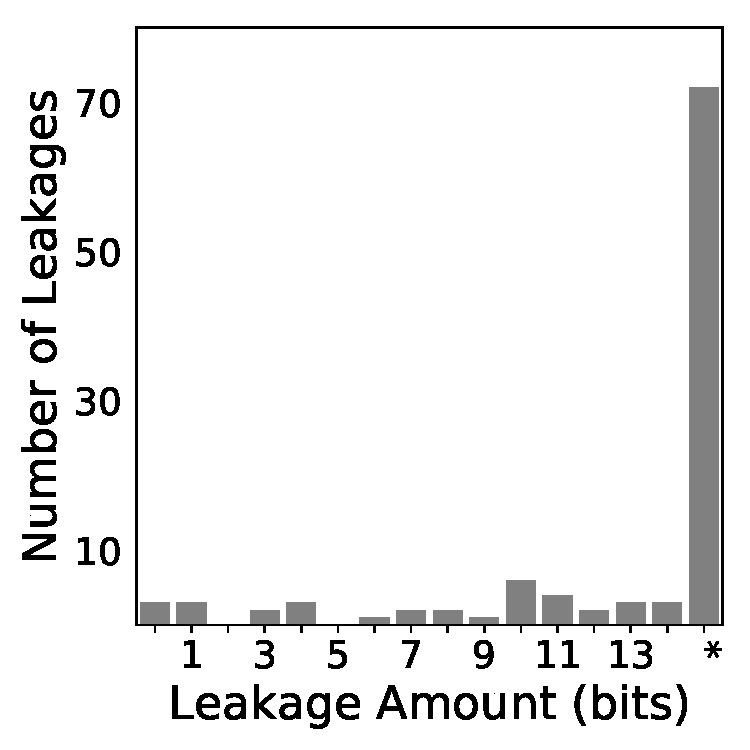
\includegraphics[width=.16\linewidth]{./figures/result/RSA-openssl-0-9-7.pdf}
        \label{fig:rsa-1}
    }
    \subfloat[OpenSSL 1.0.2f]{
        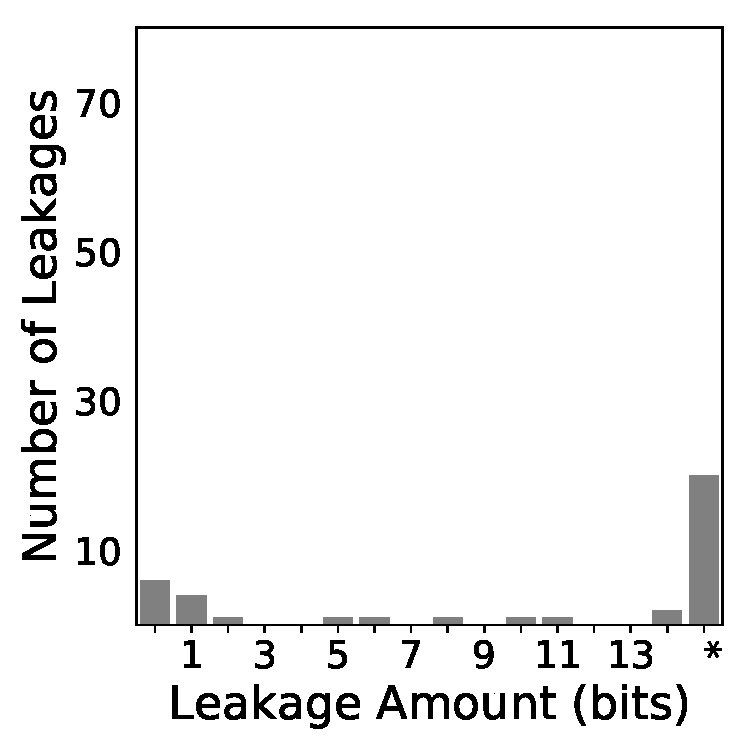
\includegraphics[width=.16\linewidth]{./figures/result/RSA-openssl-1-0-2f.pdf}
        \label{fig:rsa-2}
    }
    \subfloat[OpenSSL 1.0.2k]{
        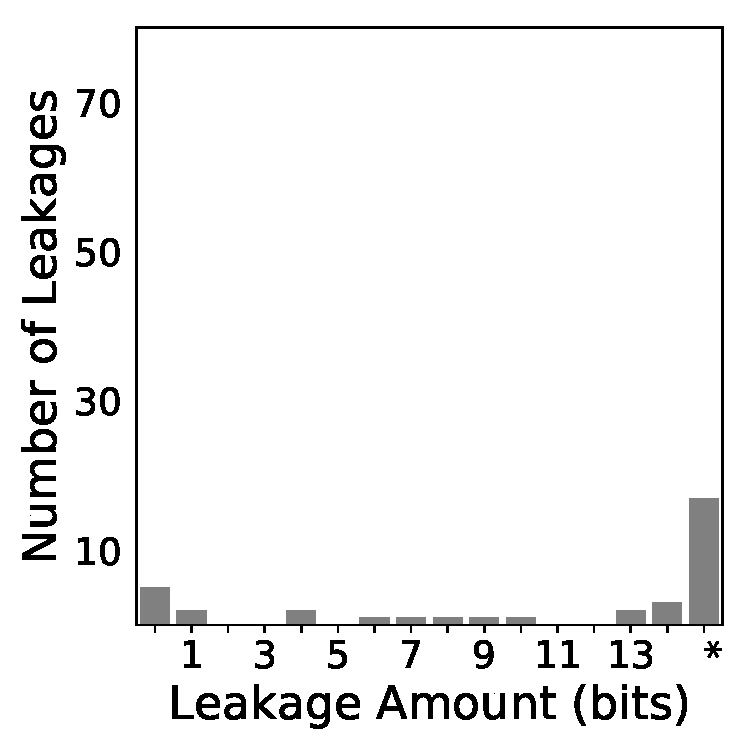
\includegraphics[width=.16\linewidth]{./figures/result/RSA-openssl-1-0-2k.pdf}
        \label{fig:rsa-3}
    }
    \subfloat[OpenSSL 1.1.0f]{
        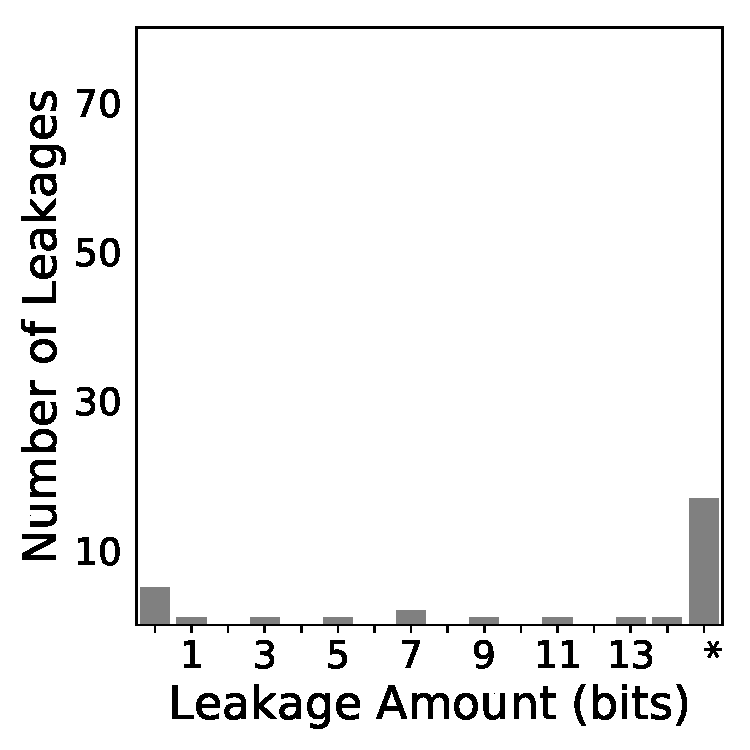
\includegraphics[width=.16\linewidth]{./figures/result/RSA-openssl-1-1-0f.pdf}
        \label{fig:rsa-4}
    }
    \subfloat[OpenSSL 1.1.1]{
        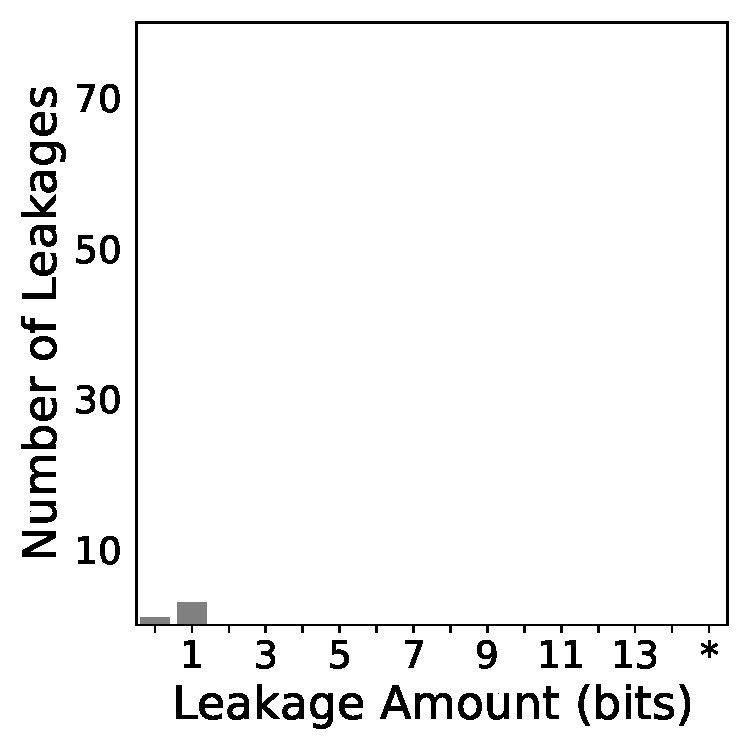
\includegraphics[width=.16\linewidth]{./figures/result/RSA-openssl-1-1-1.pdf}
        \label{fig:rsa-5}
    }
    \subfloat[OpenSSL 1.1.1g]{
        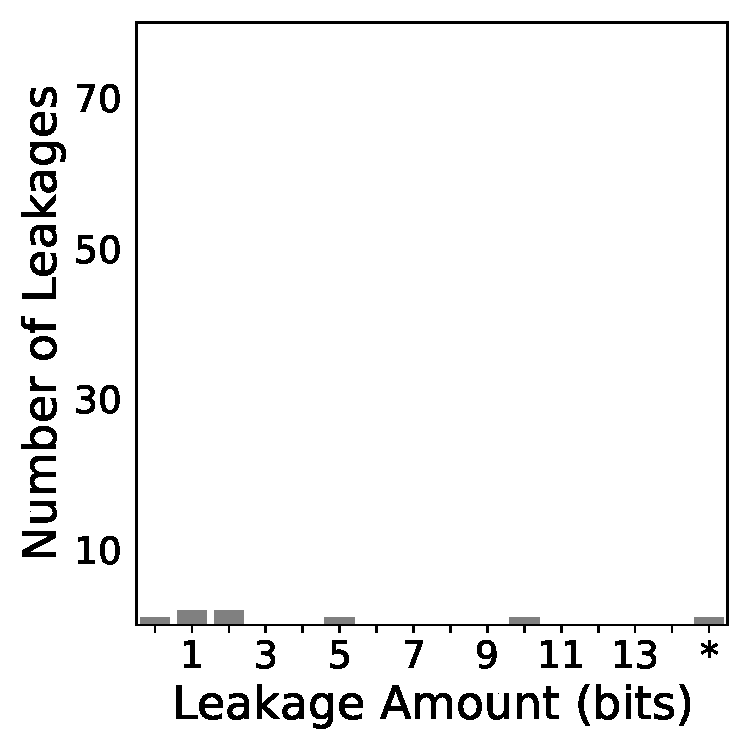
\includegraphics[width=.16\linewidth]{./figures/result/RSA-openssl-1-1-1g.pdf}
        \label{fig:rsa-6}
    }
    \caption{Side-channel leakages in different implementations of RSA in OpenSSL\@. 
        We round the number of leaked information into the nearest integer. 
        The mark $*$ means timeout (see \S\ref{loc:timeout}).}
    \label{fig:rsa}
    \vspace*{-20pt}
\end{figure*}
We also evaluate \tool{} on RSA. Due to the page limit,
we do not present the detailed leakage report. %, which is available online at the tool release website.
%% \jl{where?}. In general,
%% developers are interested in fixing side-channel vulnerabilities for the RSA implementations.
%% \jl{Then maybe find some space to present these results?}
 As shown in Figure~\ref{fig:rsa}, the result indicates that the newer
versions of OpenSSL leak less information than earlier
versions. After version 0.9.7g, OpenSSL adopts a fixed-window \textsf{mod\_exp\_mont}
implementation for RSA\@. With this design, the sequence of squares and
multiples and the memory access patterns are independent of the secret key.
\tool{}'s result confirms the new exponentiation implementation has mitigated 
most leakages effectively because the four newer versions have fewer
leakages than version 0.9.7, which introduced this change.
OpenSSL version 1.0.2f, 1.0.2k, and 1.1.0f almost have the
same amount of leakage. We check the ChangeLog and find only one change to
patch vulnerability CVE-2016-0702. 
\tool{} finds OpenSSL 1.1.1 and 1.1.1g have significantly less
leaked information than other versions.
We check the ChangeLog of these two versions and find a claim that
the new RSA implementation adopts ``numerous side-channel attack mitigation'', 
which proves the effectiveness of our quantifying method.
We also observe the latest version (1.1.1g) contains some new leakages. We have
contacted the developers and they have confirmed our findings.



Our quantification result shows vulnerabilities
that leak significant amounts of information
are more likely to be fixed in the updated version.
As presented in Figure~\ref{fig:rsa}, 
OpenSSL 0.9.7 has several severe leaks from
function \textsf{bn\_sqr\_comba8}, which is a main 
component of the OpenSSL big number implementation.
Shown in Figure~\ref{fig:old_sqr2}, it has a 
secret-dependent control flow at line 8.
The value of the function parameter \textbf{a} is derived from
the secret key. 
As function \textsf{bn\_sqr\_comba8}
calls the macro (\textsf{sqr\_add\_c2}) multiple times, 
and the code can leak some information each time.
\tool{} indicates the vulnerability is quite serious. 
It was patched in OpenSSL 1.1.1\@. In 
Figure~\ref{fig:new_sqr2}, control-flows transfers are replaced
so there are no leaks in the function
\textsf{sqr\_add\_c2} in OpenSSL 1.1.1\@. We note
that line 4 and 9 in Figure~\ref{fig:old_sqr2} both contain if branches.
However, they are not leaks because
most compilers use \emph{add with carry} instruction to eliminate the branch.
In addition, branches can be compiled into non-branch machine instructions 
with conditional moves. 
We notice a bitwise operation in Libgcrypt 1.8.5 is compiled to a conditional 
jump, which leads to a side-channel leakage.
Therefore, source-level code reviews are not accurate
enough to detect side-channels. 

For vulnerabilities that leak less information,
developers are more reluctant to fix them. 
For example, OpenSSL 0.9.7 adopts a fixed windows version of 
function \textsf{BN\_mod\_exp\_mont\_consttime} to replace original function
\textsf{BN\_mod\_exp\_mont}.
\tool{} detects a minor vulnerability in the original function that can
leak the last bit of the big number \textbf{m}. In the updated version,
developers make the fixed windows the default option and rewrite most of the 
function. However, the leakage site still exists in OpenSSL 1.1.1.
\begin{figure}
    \centering
    \begin{lstlisting}[xleftmargin=.02\textwidth,xrightmargin=.01\textwidth]
# define mul_add_c2(a,b,c0,c1,c2)                    \
    t=(BN_ULLONG)a*b;                                \
    tt=(t+t)&BN_MASK;                                \
    if (tt < t) c2++;                                \
    t1=(BN_ULONG)Lw(tt);                             \
    t2=(BN_ULONG)Hw(tt);                             \
    c0=(c0+t1)&BN_MASK2;                             \
    if ((c0 < t1) && (((++t2)&BN_MASK2) == 0)) c2++; \
    c1=(c1+t2)&BN_MASK2; if ((c1) < t2) c2++;
\end{lstlisting}
    \vspace*{-6pt}
    \caption{Macro \textsf{sqr\_add\_c2} in OpenSSL 0.9.7}
    \label{fig:old_sqr2}
    \vspace*{-8pt}
\end{figure}


\begin{figure}
    \centering
    \begin{lstlisting}[xleftmargin=.02\textwidth,xrightmargin=.01\textwidth]
# define mul_add_c2(a,b,c0,c1,c2)      do { \
    BN_ULONG ta = (a), tb = (b);            \
    BN_ULONG lo, hi, tt;                    \
    BN_UMULT_LOHI(lo,hi,ta,tb);             \
    c0 += lo; tt = hi+((c0<lo)?1:0);        \
    c1 += tt; c2 += (c1<tt)?1:0;            \
    c0 += lo; hi += (c0<lo)?1:0;            \
    c1 += hi; c2 += (c1<hi)?1:0;            \
    } while(0)
\end{lstlisting}
    \vspace*{-6pt}
    \caption{Macro \textsf{sqr\_add\_c2} in OpenSSL 1.1.1}
    \label{fig:new_sqr2}
    \vspace*{-10pt}
\end{figure}


\subsubsection{Monocypher}\label{eval:mono}
Monocypher is a small, easy to use cryptographic library with
performance comparable to LibSodium~\cite{libsodium} and NaCl~\cite{bernstein2012security}. 
We choose four ciphers that are 
designed to be side-channel resistant from the library.
Because those ciphers have no 
data flow from secrets to branch conditions and load addresses.
Monocypher should be safe under our threat models. 
We analyze those ciphers with \tool{}, and it reports no leaks.
This indicates that \tool{} is effective for validating countermeasures.

\section{Discussions and Limitations}
While recent work found many side-channel vulnerabilities, 
we note that many of them have not been patched by developers.
Side-channels are ubiquitous in software and it would be difficult to fix all of them. 
We need a tool that estimates the sensitivity of each vulnerability
so software engineers can focus on
``severe'' leakages. For example, \tool{} reports that 
the modular exponentiation using square and multiply algorithms can
leak more information than a key validation function.

Software developers can use \tool{} to find severe vulnerabilities
and reason about countermeasures.
\tool{} estimates the amount of leaked information for each side-channel leakage
in one execution trace. \tool{} is useful for software
engineers to test programs and fix vulnerabilities.
The design, which is more precise in reporting true leakages as compared with other static
methods~\cite{197207,BacelarAlmeida:2013:FVS:2483313.2483334}, obviously misses
leakages on unexplored traces. The amount of leaked information also depends on the secret key.
However, as the tool is intended for debugging and testing,
we think it is a software engineer's responsibility to select the input key and trigger 
the path in which they are interested. It is not a problem for crypto software 
since virtually all keys follow similar computational paths.

We use the amount of leaked information to represent the sensitivity level of 
each side-channel vulnerability. Although imperfect, \tool{} produces a reasonable 
measurement for each leak. For example, the simple modular exponentiation is 
notoriously famous for multiple side-channel attacks~\cite{kocher1996timing}. 
During the execution, a single leak point may execute multiple times
and each time leak a different bit. In this case, \tool{} reports that the 
vulnerability can leak the whole key. However, not every leak point inside a 
loop is severe. If a site in the loop leaks the same bit from the 
original key, and these leaks are not independent. \tool{} captures most 
fine-grained information by modeling each leak during the execution as a 
formula and the conjunction of the formulas to describe its total effect. 
Some leakage sites (e.g., square and multiply) 
can leak one particular bit of the original key, but some leakage sites leak one bit 
from several bytes in the original key. \tool{} can capture the dependency among the leaks and
reports more precise leakage information.

\tool{} reaches full precision if the number of estimated leaked bits 
equals to Definition~\ref{def}. 
\tool{} may lose precision from the 
memory model it uses in theory. However, we did not find false positives 
caused by the imprecise memory model during our evaluation. 
Sampling introduces imprecision but with a probabilistic guarantee. 
However, during the evaluation, we find that \tool{} cannot estimate 
the amount of leakage for some leakage sites in a reasonable time, 
which means the number of $K^o$ is very small. According to Definition~\ref{def}, 
it means the leakage is very severe. The sampling method in \S\ref{sec:scala} seems
simple and may miss some leakages (e.g., chosen ciphertext attacks) in theory. 
However, the evaluation result 
shows \tool{} can identify all leakages found by the previous work~\cite{203878,236338,Brotzman19Casym}.

\section{Related Work}

There is a vast amount of work on 
side channel 
detection~\cite{182946, 236338, Brotzman19Casym, 203878,217537,Wichelmann:2018:MFF:3274694.3274741,langley2010ctgrind}, 
mitigation~\cite{Page2005PartitionedCA,
Wang:2007:NCD:1250662.1250723,Zhang:2015:HDL:2775054.2694372,Li:2014:SLH:2541940.2541947,
236344,shih2017t,Coppens:2009:PMT:1607723.1608124,
brickell2006software,crane2015thwarting}, 
information
quantification~\cite{biondi2018scalable,10.1007/978-3-642-31424-7_40,McCamantE2008,5207642,Phan:2012:SQI:2382756.2382791,Chattopadhyay:2017:QIL:3127041.3127044,zhang2010sidebuster}, 
and model counting~\cite{wei2005new, gomes2007sampling, gomes2006model, kroc2008leveraging, Chattopadhyay:2017:QIL:3127041.3127044}.
Here we only present the closely related work to ours.
Due to space limit, we do not include side-channel attacks work.

\subsection{Detection and Mitigation}

There are a large number of works on side-channel vulnerability detections in
recent years.  CacheAudit~\cite{182946} uses abstract domains to compute the
over approximation of cache-based side-channel information leakage upper bound.
However, it is
less useful to judge the sensitive level of the side-channel leakage based on
the leakage provided by CacheAudit. CacheS~\cite{236338} improves the work of
CacheAudit by proposing the novel abstract domains, which only track
secret-related code. Like CacheAudit, CacheS cannot provide the information to
indicate the sensitive level of side-channel vulnerabilities.
CacheSym~\cite{Brotzman19Casym} introduces a static cache-aware symbolic
reasoning technique to cover multiple paths for the target program. Still, their
approaches cannot assess the sensitive level for each side-channel
vulnerability. And their approaches only work on small code snippets.

The dynamic approach, usually with taint analysis and symbolic execution,
can perform a very precise analysis. CacheD~\cite{203878} takes a concrete
 execution trace and run the symbolic execution on the top of the trace
to get the formula of each memory address. Therefore, CacheD is
quite precise in term of false positives. We adopted a similar idea to model the
secret-dependent memory accesses. DATA~\cite{217537} detects address-based
side-channel vulnerabilities by comparing different execution traces under
various test inputs. MicroWalk~\cite{Wichelmann:2018:MFF:3274694.3274741} uses
mutual information (MI) between sensitive input and execution state to detect
side-channels. They can only detect control-flow channels and MI scores are less
meaningful for dynamic analysis.

Both hardware~\cite{Page2005PartitionedCA,
Wang:2007:NCD:1250662.1250723,Zhang:2015:HDL:2775054.2694372,Li:2014:SLH:2541940.2541947,
236344, 236334} and software~\cite{shih2017t,Coppens:2009:PMT:1607723.1608124,
brickell2006software,crane2015thwarting, 197207} side-channels mitigation methods have
been proposed recently. Hardware countermeasures, including parting the hardware
computing resource~\cite{Page2005PartitionedCA}, randomizing cache
accesses~\cite{Wang:2007:NCD:1250662.1250723, 236344}, and designing new
architecture~\cite{tiwari2011crafting}, which need to change the hardware and is
usually hard to adopt in reality. On the contrary, software approaches are
usually easy to implement. Coppens et
al.~\cite{Coppens:2009:PMT:1607723.1608124} introduced a compiler-based approach
to eliminate key-dependent control-flow transfers. Crane et
al.~\cite{crane2015thwarting} mitigated side-channels by randomizing software.
As for crypto libraries, the basic idea is to eliminate key-dependent
control-flow transfers and data accesses. Common approaches include
bit-slicing~\cite{konighofer2008fast,rebeiro2006bitslice} and unifying
control-flows~\cite{Coppens:2009:PMT:1607723.1608124}.

\subsection{Quantification}

Proposed by Denning~\cite{robling1982cryptography} and Gray~\cite{gray1992toward}, 
Quantitative Information Flow (QIF) aims at providing an estimation of the amount of leaked
information from the sensitive information given the public output. If zero bit
of the information is leaked, the program is called non-interference. McCamant
and Ernst~\cite{McCamantE2008} quantify the information leakage as the network
flow capacity. Backes et al.~\cite{5207642} propose an automated method for QIF
by computing an equivalence relation on the set of input keys. But the approach
cannot handle real-world programs with bitwise operations. 
Phan et
al.~\cite{Phan:2012:SQI:2382756.2382791} propose symbolic QIF. The goal of their
work is to ensure the program is non-interference. They adopt an over
approximation way of estimating the total information leakage and their method
does not work for secret-dependent memory access side-channels.
CHALICE~\cite{Chattopadhyay:2017:QIL:3127041.3127044} quantifies the leaked
information for a given cache behavior. CHALICE symbolically reason about cache
behavior and estimate the amount of leaked information based on cache miss/hit.
Their approach can only scale to small programs, which limits its usage in
real-world applications. On the contrary, \tool{} can assess the sensitive level
of side-channels with different granularities. It can also analyze side-channels
in real-world crypto libraries.

\subsection{Model Counting}
Model counting usually refers to the problem of computing the number of 
models for a propositional formula (\#SAT). There are two directions
solving the problem, exact model counting and approximate model 
counting. We focus on approximate model counting since it shares similar 
idea as our approach. Wei and Selman~\cite{wei2005new} introduce
ApproxCount, a local search based method using Markov Chain Monte 
Carlo (MCMC). ApproxCount has the better scalability compared to 
exact model counters. Other approximate model counter includes 
SampleCount~\cite{gomes2007sampling},
Mbound~\cite{gomes2006model}, and MiniCount~\cite{kroc2008leveraging}. 
Compared to ApproxCount,
those model counters can give lower or upper bounds with guarantees.
Despite the rapid development of model counters for SAT and some 
research~\cite{chistikov2017approximate,phan2015model} on Modulo Theories model counting (\#SMT).
They cannot be directly applied to 
side channel leakage quantification.
ApproxFlow~\cite{biondi2018scalable} uses ApproxMC~\cite{chakraborty2016algorithmic} for information flow quantification,
but it's only tested with small programs while \tool\ can scale to production crypto libraries. 




\section{Conclusion}
In this paper, we present a novel information leakage %definition and
method to
quantify memory-based side-channel leakages. We implement the method in
a prototype called \tool{} and show that it is effective in finding
and quantifying the side-channel leakages. With the new definition of
information leakage that imitates real side-channel attackers, the number of
leaked bits is useful in practice to justify and understand the severity level
of side-channel vulnerabilities. The evaluation results confirm our design goal
and show \tool{} is useful in estimating the amount of leaked information in
real-world applications.

\newpage

\bibliographystyle{IEEEtran}
\bibliography{refs}

\newpage
\clearpage
%\appendices
\setcounter{section}{0}
\section*{Supplementary Materials to Submission \#63}
%\setcounter{section}{1}
\setcounter{page}{1}

\newcommand{\vvv}{\vspace*{-3pt}}

\section{\tool{}' main components}

\label{appendix:code}
\begin{table}[h!]
    \centering
    %    \resizebox{.8\columnwidth}{!}{
    \caption{\tool{}' main components and sizes}\label{tbl:implementation}
    \begin{tabular}{lr@{~}@{}l}
        \hline
        Component            & \multicolumn{2}{c}{Lines of Code (LOC)}             \\ \hline
        Trace Logging        & 501 lines                               & of C++    \\
        Symbolic Execution   & 14,963 lines                            & of C++    \\
        Data Flow            & 451 lines                               & of C++    \\
        Monte Carlo Sampling & 603 lines                               & of C++    \\
        Others               & 211 lines                               & of Python \\ \hline
        Total                & 16,729 lines                            &           \\\hline
    \end{tabular}
    %    }
\end{table}



\section{Algorithm to Compute the Maximum Independent Partition}
\label{appendix:partition}
~
{\small
\IncMargin{1em}
\begin{algorithm}[h]\small
    \DontPrintSemicolon
    \SetKwInOut{Input}{input}\SetKwInOut{Output}{output}
    \Input{$c_t(\addr{1},\addr{2},\ldots,\addr{n}) = c_{\addr{1}} \land c_{\addr{2}} \land \ldots \land c_{\addr{m}}$}
    \Output{The Maximum Independent Partition of $G = \{g_{1}, g_{2}  , \ldots,  g_{m} \}$ }
    \For{$i\leftarrow 1$ \KwTo $n$}
    {
        $S_{c_{\addr{i}}}$ $\leftarrow$ $\pi(c_{\addr{i}})$ \;
        \For{$g_{i} \in G$}
        {
            $S_{g_j}$ $\leftarrow$ $\pi(g_{j})$ \;
            $S$ $\leftarrow$ $S_{c_{\addr{i}}} \cap S_{g_j}$  \;
            \If{$S \neq \emptyset$}
            {
                $g_{j} \leftarrow g_{i} \land g_{\addr{i}}$ \;
                \textbf{break} \;
            }
            Insert $c_{\addr{i}}$ to $G$
        }
    }
    \caption{The Maximum Independent Partition}
    \label{algo:max-inde}
\end{algorithm}
\DecMargin{1em}
}
~
\newpage
\section{Algorithm to Compute the Number of Satisfying Assignments}
\label{appendix:montecarlo}
~
{\small
\IncMargin{1em}
\begin{algorithm}\small
    \SetAlgoLined
    \DontPrintSemicolon

    \KwIn{{The constraint $g_{i}= c_{i_1} \land c_{i_2}
                    \land \ldots \land c_{i_m}$}}
    \KwOut{{The number of assignments that satisfy $g_{i}$ $|K_{g_{i}}|$}}

    $n$: the number of sampling times \;
    $S_{c_i}$: the set contains input variables for $c_{i}$ \;
    $n_{s}$: the number of satisfying assignments \;
    $N_{c_t}$: the set contains all solution for $c_t$ \;
    $r$: times of reducing $g$\;
    $k$: the input variable \;
    $R$: a function that produces a random point from $S_{c_i}$\;
    %$\#k$: the satisfying number of k \fixme{this number is not used syntactically} \;
    %Initialization: \;
    $r$ $\leftarrow$ $1$,
    $n$ $\leftarrow$ $0$ \;
    \For{$t$ $\leftarrow$ $1$ \KwTo $m$} {
        $S_{c_t}$ $\leftarrow$ $\pi(c_t)$ \;
        \If{$|S_{c_t}| = 1$}
        {
            $N_{c_t}$ $\leftarrow$ Compute all solutions of $c_i$ \;
            $N_{c_t} = \{n_1, \ldots, n_m\},\ S_{c_t} = \{k\}  $ \;
            $g_{i} = $ $g_i(k=n_1) \land \ldots \land g_i(k=n_m)$ \;
            $r \leftarrow r+1$ \;

        }
    }
    \While{$n \leq \frac{6p}{1-p}$} {
        $S_{g_i}$ $\leftarrow$ $\pi(g_i)$ \;
        $v \leftarrow R(S_{g_i})$ 
        \If{$v$ satisfies $g_i$}
        {
           $n_s \leftarrow n_s + 1$
        }
        $n \leftarrow n +1,\ p = \frac{n_s}{n}$
    }

    $|K_{g_{i}}|$ $\leftarrow$ $n_s|K| / (n * r * range(k))$
    \caption{Multiple Step Monte Carlo Sampling}
\end{algorithm}
\DecMargin{1em}
}
~\vvv

\section{AES Lookup Tables Leakage}
\begin{figure}[h!]
    \centering
    \begin{lstlisting}[xleftmargin=.01\textwidth,xrightmargin=.01\textwidth]
int mbedtls_internal_aes_encrypt( mbedtls_aes_context *ctx,
const unsigned char input[16],
unsigned char output[16] )
{
uint32_t *RK, X0, X1, X2, X3, Y0, Y1, Y2, Y3;
...
for( i = ( ctx->nr >> 1 ) - 1; i > 0; i-- )
{
  AES_FROUND( Y0, Y1, Y2, Y3, X0, X1, X2, X3 ); // Leakage 1
  AES_FROUND( X0, X1, X2, X3, Y0, Y1, Y2, Y3 ); // Leakage 2
}
AES_FROUND( Y0, Y1, Y2, Y3, X0, X1, X2, X3 );   // Leakage 3
X0 = *RK++ ^ \                                  // Leakage 4
    ( (uint32_t) FSb[ ( Y0       ) & 0xFF ]       ) ^
    ( (uint32_t) FSb[ ( Y1 >>  8 ) & 0xFF ] <<  8 ) ^
    ( (uint32_t) FSb[ ( Y2 >> 16 ) & 0xFF ] << 16 ) ^
    ( (uint32_t) FSb[ ( Y3 >> 24 ) & 0xFF ] << 24 );
// X1, X2, X3 do the same computation as X0
...                                          // Leakage 5,6,7
PUT_UINT32_LE( X0, output,  0 );
...
return( 0 );
}
\end{lstlisting}
    \vspace*{-6pt}
    \caption{Function \textit{mbedtls\_internal\_aes\_encrypt}}
    \label{mbedtls_aes}
    \vspace*{-9pt}
\end{figure}

\clearpage
\section{Minor side-channels vulnerability}
\label{appendix:minor:vul}
Here we present a side-channel vulnerability that leaks
less than one bit information by~\tool{}. The vulnerability exists
from OpenSSL 0.9.7 to OpenSSL 1.1.1. We think
developers do not have enough motivations
to fix the vulnerability.

\begin{figure}[h]
\centering
\begin{lstlisting}[xleftmargin=.02\textwidth,xrightmargin=.01\textwidth]
int BN_mod_exp_mont_consttime(BIGNUM *rr, 
const BIGNUM *a, const BIGNUM *p,
const BIGNUM *m, BN_CTX *ctx, BN_MONT_CTX *in_mont)
{
... 
if (!(m->d[0] & 1)) {
    ... 
    return 0;
}
bits = BN_num_bits(p);
if (bits == 0) 
...
}
\end{lstlisting}
    \vspace*{-6pt}
    \caption{\emph{BN\_mod\_exp\_mont\_consttime} in OpenSSL 0.9.7}
    \label{fig:old_sqr2}
    \vspace*{-6pt}
\end{figure}



\begin{figure}[h]
    \centering
    \begin{lstlisting}[xleftmargin=.02\textwidth,xrightmargin=.01\textwidth]
int BN_mod_exp_mont(BIGNUM *rr, 
const BIGNUM *a, const BIGNUM *p,
const BIGNUM *m, BN_CTX *ctx, BN_MONT_CTX *in_mont)
{
...
if (!BN_is_odd(m)) {
    ...
    return 0;
}
bits = BN_num_bits(p);
if (bits == 0) 
...
}

\end{lstlisting}
    \vspace*{-6pt}
    \caption{\emph{BN\_mod\_exp\_mont} in OpenSSL 1.1.1}
    \label{fig:new_sqr2}
    \vspace*{-6pt}
\end{figure}

\section{Unknown Leaks in OpenSSL 1.1.1}

\section{Detailed Experimental Results}
\label{sec:result-table}

Here we present the detailed experimental results.
Due to space limitation, we select the representative implementations of
AES, DES, and RSA in
mbed TLS 2.5,
OpenSSL 1.1.0f,  and
OpenSSL 1.1.1.  
%For RSA, we also include OpenSSL 1.0.2f and OpenSSL 1.0.2k.
The results are representative to other versions.
All the results will be made available in electronic format online
when the paper is published. %at \fixme{http://tinyurl}.

In all the tables presented in this appendix, the mark ``$*$'' means timeout,
which indicates more severe leakages. See \S\ref{loc:timeout} for the details.
Also note that we round the calculated numbers of leaked bits to include one digit
after the decimal point, so $0.0$ really means very small amount of leakage, but not exactly zero. See \S\ref{sssec:errest} for the details of error estimate.

  %as an integer.
  %Hence the `0' leakage does not equals to no leakage but some leakage size
 % between 0 and 0.5 bit, see \S\ref{sssec:errest} for the details.


\begin{table}[!ht]
\centering\tiny\scriptsize
\caption{Leakages in DES implemented by mbed TLS 2.5}\label{tab:DESmbed TLS2.5}
%\resizebox{\columnwidth}{!}{
\begin{tabular}{lrlrr}
\hline
\textbf{File} & \textbf{Line No.} & \textbf{Function} & \textbf{\# Leaked Bits} & \textbf{Type} \\\hline
des.c& 441&mbedtls\_des\_setkey&0.9 &DA\\
des.c& 438&mbedtls\_des\_setkey&1.0 &DA\\
des.c& 438&mbedtls\_des\_setkey&1.0 &DA\\
des.c& 439&mbedtls\_des\_setkey&1.1 &DA\\
des.c& 439&mbedtls\_des\_setkey&1.0 &DA\\
des.c& 440&mbedtls\_des\_setkey&1.0 &DA\\
des.c& 446&mbedtls\_des\_setkey&0.9 &DA\\
des.c& 446&mbedtls\_des\_setkey&1.0 &DA\\
des.c& 444&mbedtls\_des\_setkey&1.0 &DA\\
des.c& 444&mbedtls\_des\_setkey&1.0 &DA\\
des.c& 443&mbedtls\_des\_setkey&1.0 &DA\\
des.c& 443&mbedtls\_des\_setkey&1.0 &DA\\
des.c& 444&mbedtls\_des\_setkey&1.0 &DA\\
des.c& 445&mbedtls\_des\_setkey&1.1 &DA\\
des.c& 448&mbedtls\_des\_setkey&0.9 &DA\\
\hline
\end{tabular}
%}
\renewcommand{\baselinestretch}{1.0}\selectfont
\end{table}

%% \begin{table}[!ht]
\centering\tiny\scriptsize
\caption{Leakages in DES implemented by mbed TLS 2.15.1}\label{tab:DESmbed TLS2.15.1}
%\resizebox{\columnwidth}{!}{
\begin{tabular}{lrlrr}
\hline
\textbf{File} & \textbf{Line No.} & \textbf{Function} & \textbf{\# Leaked Bits} & \textbf{Type} \\\hline
des.c& 437&mbedtls\_des\_setkey&1.0 &DA\\
des.c& 434&mbedtls\_des\_setkey&1.0 &DA\\
des.c& 434&mbedtls\_des\_setkey&1.0 &DA\\
des.c& 435&mbedtls\_des\_setkey&1.0 &DA\\
des.c& 435&mbedtls\_des\_setkey&1.0 &DA\\
des.c& 436&mbedtls\_des\_setkey&1.0 &DA\\
des.c& 442&mbedtls\_des\_setkey&1.0 &DA\\
des.c& 442&mbedtls\_des\_setkey&1.0 &DA\\
des.c& 440&mbedtls\_des\_setkey&0.9 &DA\\
des.c& 440&mbedtls\_des\_setkey&1.0 &DA\\
des.c& 439&mbedtls\_des\_setkey&1.0 &DA\\
des.c& 439&mbedtls\_des\_setkey&0.9 &DA\\
des.c& 440&mbedtls\_des\_setkey&1.0 &DA\\
des.c& 441&mbedtls\_des\_setkey&1.0 &DA\\
des.c& 444&mbedtls\_des\_setkey&0.9 &DA\\
\hline
\end{tabular}
%}
\renewcommand{\baselinestretch}{1.0}\selectfont
\end{table}

%% \begin{table}[!ht]
\centering\tiny\scriptsize
\caption{Leakages in DES implemented by OpenSSL 0.9.7}\label{tab:DESOpenSSL0.9.7}
%\resizebox{\columnwidth}{!}{
\begin{tabular}{lrlrr}
\hline
\textbf{File} & \textbf{Line No.} & \textbf{Function} & \textbf{\# Leaked Bits} & \textbf{Type} \\\hline
set\_key.c& 380&DES\_set\_key\_unchecked&5.7 &DA\\
set\_key.c& 380&DES\_set\_key\_unchecked&6.6 &DA\\
set\_key.c& 380&DES\_set\_key\_unchecked&7.6 &DA\\
set\_key.c& 380&DES\_set\_key\_unchecked&6.5 &DA\\
set\_key.c& 385&DES\_set\_key\_unchecked&3.2 &DA\\
set\_key.c& 385&DES\_set\_key\_unchecked&1.9 &DA\\
\hline
\end{tabular}
%}
\renewcommand{\baselinestretch}{1.0}\selectfont
\end{table}

%% \begin{table}[!ht]
\centering\tiny\scriptsize
\caption{Leakages in DES implemented by OpenSSL 1.0.2f}\label{tab:DESOpenSSL1.0.2f}
%\resizebox{\columnwidth}{!}{
\begin{tabular}{lrlrr}
\hline
\textbf{File} & \textbf{Line No.} & \textbf{Function} & \textbf{\# Leaked Bits} & \textbf{Type} \\\hline
set\_key.c& 409&DES\_set\_key\_unchecked&9.8 &DA\\
set\_key.c& 417&DES\_set\_key\_unchecked&9.2 &DA\\
set\_key.c& 418&DES\_set\_key\_unchecked&8.0 &DA\\
set\_key.c& 423&DES\_set\_key\_unchecked&5.4 &DA\\
set\_key.c& 420&DES\_set\_key\_unchecked&2.0 &DA\\
set\_key.c& 422&DES\_set\_key\_unchecked&3.4 &DA\\
set\_key.c& 422&DES\_set\_key\_unchecked&2.9 &DA\\
set\_key.c& 425&DES\_set\_key\_unchecked&0.2 &DA\\
\hline
\end{tabular}
%}
\renewcommand{\baselinestretch}{1.0}\selectfont
\end{table}

%% \begin{table}[h!]
\centering\tiny\scriptsize
\caption{Leakages in DES implemented by OpenSSL 1.0.2k}\label{tab:DESOpenSSL1.0.2k}
%\resizebox{\columnwidth}{!}{
\begin{tabular}{lrlrr}
\hline
\textbf{File} & \textbf{Line No.} & \textbf{Function} & \textbf{\# Leaked Bits} & \textbf{Type} \\\hline
set\_key.c& 409&DES\_set\_key\_unchecked&8.2 &DA\\
set\_key.c& 417&DES\_set\_key\_unchecked&10.1 &DA\\
set\_key.c& 418&DES\_set\_key\_unchecked&8.1 &DA\\
set\_key.c& 423&DES\_set\_key\_unchecked&5.7 &DA\\
set\_key.c& 420&DES\_set\_key\_unchecked&3.5 &DA\\
set\_key.c& 422&DES\_set\_key\_unchecked&4.1 &DA\\
set\_key.c& 422&DES\_set\_key\_unchecked&3.6 &DA\\
set\_key.c& 425&DES\_set\_key\_unchecked&0.7 &DA\\
\hline
\end{tabular}
%}
\renewcommand{\baselinestretch}{1.0}\selectfont
\end{table}

\begin{table}[h!]
\centering\tiny\scriptsize
\caption{Leakages in DES implemented by OpenSSL 1.1.0f}\label{tab:DESOpenSSL1.1.0f}
%\resizebox{\columnwidth}{!}{
\begin{tabular}{lrlrr}
\hline
\textbf{File} & \textbf{Line No.} & \textbf{Function} & \textbf{\# Leaked Bits} & \textbf{Type} \\\hline
set\_key.c& 351&DES\_set\_key\_unchecked&7.1 &DA\\
set\_key.c& 353&DES\_set\_key\_unchecked&8.8 &DA\\
set\_key.c& 361&DES\_set\_key\_unchecked&8.0 &DA\\
set\_key.c& 362&DES\_set\_key\_unchecked&5.7 &DA\\
set\_key.c& 362&DES\_set\_key\_unchecked&2.0 &DA\\
set\_key.c& 364&DES\_set\_key\_unchecked&3.5 &DA\\
set\_key.c& 364&DES\_set\_key\_unchecked&4.9 &DA\\
set\_key.c& 365&DES\_set\_key\_unchecked&0.4 &DA\\
\hline
\end{tabular}
%}
\renewcommand{\baselinestretch}{1.0}\selectfont
\end{table}

\begin{table}[!ht]
\centering\tiny\scriptsize
\caption{Leakages in DES implemented by OpenSSL 1.1.1}\label{tab:DESOpenSSL1.1.1}
%\resizebox{\columnwidth}{!}{
\begin{tabular}{lrlrr}
\hline
\textbf{File} & \textbf{Line No.} & \textbf{Function} & \textbf{\# Leaked Bits} & \textbf{Type} \\\hline
set\_key.c& 350&DES\_set\_key\_unchecked&5.8 &DA\\
set\_key.c& 350&DES\_set\_key\_unchecked&6.6 &DA\\
set\_key.c& 350&DES\_set\_key\_unchecked&7.5 &DA\\
set\_key.c& 350&DES\_set\_key\_unchecked&6.4 &DA\\
set\_key.c& 355&DES\_set\_key\_unchecked&1.9 &DA\\
set\_key.c& 355&DES\_set\_key\_unchecked&3.1 &DA\\
\hline
\end{tabular}
%}
\renewcommand{\baselinestretch}{1.0}\selectfont
\end{table}



\begin{table}[!ht]
\centering\tiny\scriptsize
\caption{Leakages in RSA implemented by mbed TLS 2.5}\label{tab:RSAmbed TLS2.5}
%\resizebox{\columnwidth}{!}{
\begin{tabular}{lrlrr}
\hline
\textbf{File} & \textbf{Line No.} & \textbf{Function} & \textbf{\# Leaked Bits} & \textbf{Type} \\\hline
bignum.c& 1617&mbedtls\_mpi\_exp\_mod&0.9 &CF\\
bignum.c& 861&mbedtls\_mpi\_cmp\_mpi&8.5 &CF\\
bignum.c& 862&mbedtls\_mpi\_cmp\_mpi&7.7 &CF\\
bignum.c& 1167&mpi\_mul\_hlp&*&CF\\
bignum.c& 828&mbedtls\_mpi\_cmp\_abs&9.6 &CF\\
bignum.c& 829&mbedtls\_mpi\_cmp\_abs&9.5 &CF\\
\hline
\end{tabular}
%}
\renewcommand{\baselinestretch}{1.0}\selectfont
\end{table}

%% \begin{table}[h!]
\centering\tiny\scriptsize
\caption{Leakages in RSA implemented by mbed TLS 2.15.1}\label{tab:RSAmbed TLS2.15.1}
%\resizebox{\columnwidth}{!}{
\begin{tabular}{lrlrr}
\hline
\textbf{File} & \textbf{Line No.} & \textbf{Function} & \textbf{\# Leaked Bits} & \textbf{Type} \\\hline
bignum.c& 855&mbedtls\_mpi\_cmp\_mpi&*&CF\\
rsa.c& 184&rsa\_check\_context.isra.0&1.0 &CF\\
bignum.c& 825&mbedtls\_mpi\_cmp\_abs&*&CF\\
bignum.c& 197&mbedtls\_mpi\_copy&*&CF\\
bignum.c& 1629&mbedtls\_mpi\_exp\_mod&0.9 &CF\\
bignum.c& 829&mbedtls\_mpi\_cmp\_abs&*&CF\\
bignum.c& 859&mbedtls\_mpi\_cmp\_mpi&*&CF\\
bignum.c& 873&mbedtls\_mpi\_cmp\_mpi&2.8 &CF\\
bignum.c& 874&mbedtls\_mpi\_cmp\_mpi&2.7 &CF\\
bignum.c& 840&mbedtls\_mpi\_cmp\_abs&8.2 &CF\\
bignum.c& 841&mbedtls\_mpi\_cmp\_abs&8.7 &CF\\
bignum.c& 1201&mbedtls\_mpi\_mul\_mpi&*&CF\\
\hline
\end{tabular}
%}
\renewcommand{\baselinestretch}{1.0}\selectfont
\end{table}

%%\begin{table}[h!]
\centering\tiny\scriptsize
\caption{Leakages in RSA implemented by OpenSSL 0.9.7}\label{tab:RSAOpenSSL0.9.7}
%\resizebox{\columnwidth}{!}{
\begin{tabular}{lrlrr}
\hline
\textbf{File} & \textbf{Line No.} & \textbf{Function} & \textbf{\# Leaked Bits} & \textbf{Type} \\\hline
bn\_lib.c& 228&BN\_num\_bits&0.0 &CF\\
bn\_lib.c& 229&BN\_num\_bits&4.1 &DA\\
bn\_shift.c& 152&BN\_lshift&1.0 &CF\\
bn\_lib.c& 670&BN\_ucmp&*&CF\\
a\_gentm.c& 246&\_\_udivdi3&*&CF\\
bn\_div.c& 303&BN\_div&*&CF\\
bn\_add.c& 222&BN\_usub&4.2 &CF\\
bn\_add.c& 256&BN\_usub&*&CF\\
bn\_add.c& 256&BN\_usub&*&CF\\
bn\_gcd.c& 247&BN\_mod\_inverse&1.0 &CF\\
bn\_gcd.c& 268&BN\_mod\_inverse&6.8 &CF\\
bn\_gcd.c& 287&BN\_mod\_inverse&4.4 &CF\\
bn\_gcd.c& 291&BN\_mod\_inverse&15.2 &CF\\
bn\_gcd.c& 272&BN\_mod\_inverse&12.3 &CF\\
bn\_lib.c& 670&BN\_ucmp&*&CF\\
bn\_div.c& 303&BN\_div&*&CF\\
bn\_div.c& 307&BN\_div&*&CF\\
bn\_exp.c& 590&BN\_mod\_exp\_mont\_consttime&1.0 &CF\\
bn\_mont.c& 218&BN\_from\_montgomery&*&CF\\
bn\_asm.c& 691&bn\_sqr\_comba8&*&CF\\
bn\_asm.c& 696&bn\_sqr\_comba8&12.8 &CF\\
bn\_asm.c& 696&bn\_sqr\_comba8&10.5 &CF\\
bn\_asm.c& 704&bn\_sqr\_comba8&*&CF\\
bn\_asm.c& 709&bn\_sqr\_comba8&*&CF\\
bn\_asm.c& 709&bn\_sqr\_comba8&12.8 &CF\\
bn\_asm.c& 710&bn\_sqr\_comba8&14.0 &CF\\
bn\_asm.c& 714&bn\_sqr\_comba8&*&CF\\
bn\_asm.c& 714&bn\_sqr\_comba8&7.4 &CF\\
bn\_asm.c& 715&bn\_sqr\_comba8&*&CF\\
bn\_asm.c& 718&bn\_sqr\_comba8&15.6 &CF\\
bn\_asm.c& 718&bn\_sqr\_comba8&10.9 &CF\\
bn\_asm.c& 720&bn\_sqr\_comba8&*&CF\\
bn\_asm.c& 721&bn\_sqr\_comba8&*&CF\\
bn\_asm.c& 727&bn\_sqr\_comba8&*&CF\\
bn\_asm.c& 728&bn\_sqr\_comba8&*&CF\\
bn\_asm.c& 728&bn\_sqr\_comba8&*&CF\\
bn\_asm.c& 730&bn\_sqr\_comba8&12.1 &CF\\
bn\_asm.c& 730&bn\_sqr\_comba8&9.2 &CF\\
bn\_asm.c& 731&bn\_sqr\_comba8&*&CF\\
bn\_asm.c& 732&bn\_sqr\_comba8&*&CF\\
bn\_asm.c& 733&bn\_sqr\_comba8&*&CF\\
bn\_asm.c& 737&bn\_sqr\_comba8&*&CF\\
bn\_asm.c& 738&bn\_sqr\_comba8&*&CF\\
bn\_asm.c& 738&bn\_sqr\_comba8&*&CF\\
bn\_asm.c& 740&bn\_sqr\_comba8&*&CF\\
bn\_asm.c& 740&bn\_sqr\_comba8&*&CF\\
bn\_asm.c& 746&bn\_sqr\_comba8&*&CF\\
bn\_asm.c& 748&bn\_sqr\_comba8&*&CF\\
bn\_asm.c& 748&bn\_sqr\_comba8&*&CF\\
bn\_asm.c& 692&bn\_sqr\_comba8&*&CF\\
bn\_asm.c& 698&bn\_sqr\_comba8&16.2 &CF\\
bn\_asm.c& 698&bn\_sqr\_comba8&12.1 &CF\\
bn\_asm.c& 705&bn\_sqr\_comba8&*&CF\\
bn\_asm.c& 707&bn\_sqr\_comba8&*&CF\\
bn\_asm.c& 707&bn\_sqr\_comba8&*&CF\\
bn\_asm.c& 716&bn\_sqr\_comba8&*&CF\\
bn\_asm.c& 719&bn\_sqr\_comba8&*&CF\\
bn\_asm.c& 720&bn\_sqr\_comba8&*&CF\\
bn\_asm.c& 721&bn\_sqr\_comba8&*&CF\\
bn\_asm.c& 722&bn\_sqr\_comba8&*&CF\\
bn\_asm.c& 726&bn\_sqr\_comba8&*&CF\\
bn\_asm.c& 727&bn\_sqr\_comba8&*&CF\\
bn\_asm.c& 714&bn\_sqr\_comba8&*&CF\\
bn\_asm.c& 715&bn\_sqr\_comba8&*&CF\\
bn\_asm.c& 716&bn\_sqr\_comba8&*&CF\\
bn\_asm.c& 721&bn\_sqr\_comba8&12.6 &CF\\
bn\_asm.c& 722&bn\_sqr\_comba8&*&CF\\
bn\_asm.c& 726&bn\_sqr\_comba8&*&CF\\
bn\_asm.c& 732&bn\_sqr\_comba8&*&CF\\
bn\_asm.c& 733&bn\_sqr\_comba8&*&CF\\
bn\_asm.c& 737&bn\_sqr\_comba8&*&CF\\
bn\_asm.c& 741&bn\_sqr\_comba8&*&CF\\
bn\_asm.c& 742&bn\_sqr\_comba8&*&CF\\
bn\_asm.c& 742&bn\_sqr\_comba8&*&CF\\
bn\_asm.c& 746&bn\_sqr\_comba8&*&CF\\
bn\_asm.c& 749&bn\_sqr\_comba8&*&CF\\
bn\_asm.c& 700&bn\_sqr\_comba8&17.2 &CF\\
bn\_asm.c& 700&bn\_sqr\_comba8&14.6 &CF\\
bn\_asm.c& 704&bn\_sqr\_comba8&*&CF\\
bn\_asm.c& 726&bn\_sqr\_comba8&9.0 &CF\\
bn\_asm.c& 737&bn\_sqr\_comba8&*&CF\\
bn\_asm.c& 720&bn\_sqr\_comba8&*&CF\\
bn\_asm.c& 742&bn\_sqr\_comba8&*&CF\\
bn\_asm.c& 732&bn\_sqr\_comba8&*&CF\\
bn\_asm.c& 716&bn\_sqr\_comba8&*&CF\\
bn\_asm.c& 727&bn\_sqr\_comba8&*&CF\\
bn\_asm.c& 691&bn\_sqr\_comba8&11.2 &CF\\
bn\_asm.c& 696&bn\_sqr\_comba8&*&CF\\
bn\_asm.c& 699&bn\_sqr\_comba8&*&CF\\
bn\_asm.c& 700&bn\_sqr\_comba8&*&CF\\
bn\_asm.c& 704&bn\_sqr\_comba8&*&CF\\
bn\_asm.c& 705&bn\_sqr\_comba8&*&CF\\
bn\_asm.c& 708&bn\_sqr\_comba8&*&CF\\
bn\_asm.c& 709&bn\_sqr\_comba8&*&CF\\
bn\_asm.c& 710&bn\_sqr\_comba8&*&CF\\
bn\_asm.c& 722&bn\_sqr\_comba8&10.2 &CF\\
bn\_asm.c& 705&bn\_sqr\_comba8&15.6 &CF\\
bn\_asm.c& 738&bn\_sqr\_comba8&5.4 &CF\\
bn\_asm.c& 746&bn\_sqr\_comba8&8.2 &CF\\
bn\_asm.c& 728&bn\_sqr\_comba8&10.3 &CF\\
bn\_asm.c& 715&bn\_sqr\_comba8&13.8 &CF\\
bn\_asm.c& 733&bn\_sqr\_comba8&12.2 &CF\\
bn\_asm.c& 710&bn\_sqr\_comba8&9.7 &CF\\
bn\_div.c& 303&BN\_div&1.3 &CF\\
bn\_div.c& 303&BN\_div&1.2 &CF\\
bn\_lib.c& 228&BN\_bn2bin&3.1 &CF\\
bn\_lib.c& 230&BN\_bn2bin&5.0 &DA\\
\hline
\end{tabular}
%}
\renewcommand{\baselinestretch}{1.0}\selectfont
\end{table}

\begin{table}[h!]
\centering\tiny\scriptsize
\caption{Leakages in RSA implemented by OpenSSL 1.0.2f}\label{tab:RSAOpenSSL1.0.2f}
%\resizebox{\columnwidth}{!}{
\begin{tabular}{lrlrr}
\hline
\textbf{File} & \textbf{Line No.} & \textbf{Function} & \textbf{\# Leaked Bits} & \textbf{Type} \\\hline
bn\_lib.c& 199&BN\_num\_bits&*&CF\\
bn\_lib.c& 200&BN\_num\_bits&15.6 &CF\\
bn\_lib.c& 201&BN\_num\_bits&16.2 &DA\\
bn\_lib.c& 673&BN\_ucmp&*&CF\\
bio\_asn1.c& 482&\_\_udivdi3&8.5 &CF\\
bn\_div.c& 381&BN\_div&*&CF\\
bn\_div.c& 456&BN\_div&*&CF\\
bn\_gcd.c& 279&BN\_mod\_inverse&1.0 &CF\\
bn\_gcd.c& 302&BN\_mod\_inverse&5.0 &CF\\
bn\_gcd.c& 324&BN\_mod\_inverse&6.6 &CF\\
bn\_add.c& 255&BN\_usub&*&CF\\
bn\_gcd.c& 305&BN\_mod\_inverse&12.8 &CF\\
bn\_gcd.c& 327&BN\_mod\_inverse&15.6 &CF\\
bn\_lib.c& 203&BN\_num\_bits&15.2 &DA\\
bn\_lib.c& 208&BN\_num\_bits&12.7 &CF\\
bn\_lib.c& 209&BN\_num\_bits&*&DA\\
bn\_lib.c& 212&BN\_num\_bits&*&DA\\
bn\_gcd.c& 515&BN\_mod\_inverse&*&CF\\
bn\_div.c& 381&BN\_div&2.7 &CF\\
bn\_div.c& 439&BN\_div&14.2 &CF\\
bn\_div.c& 385&BN\_div&11.4 &CF\\
bn\_div.c& 381&BN\_div&1.1 &CF\\
bn\_div.c& 381&BN\_div&1.0 &CF\\
bn\_div.c& 469&BN\_div&0.9 &CF\\
bn\_exp.c& 676&BN\_mod\_exp\_mont\_consttime&1.0 &CF\\
bn\_exp.c& 796&BN\_mod\_exp\_mont\_consttime&1.0 &CF\\
bn\_mont.c& 262&BN\_from\_montgomery\_word&*&DA\\
bn\_mont.c& 263&BN\_from\_montgomery\_word&*&DA\\
bn\_mont.c& 264&BN\_from\_montgomery\_word&*&DA\\
bn\_mont.c& 266&BN\_from\_montgomery\_word&*&DA\\
bn\_mont.c& 276&BN\_from\_montgomery\_word&*&DA\\
bn\_mont.c& 276&BN\_from\_montgomery\_word&0.2 &DA\\
bn\_mont.c& 276&BN\_from\_montgomery\_word&0.2 &DA\\
bn\_mont.c& 275&BN\_from\_montgomery\_word&0.1 &CF\\
bn\_mont.c& 282&BN\_from\_montgomery\_word&*&CF\\
bn\_asm.c& 787&bn\_sqr\_comba8&*&CF\\
bn\_asm.c& 646&bn\_mul\_comba8&*&CF\\
bn\_mont.c& 201&BN\_from\_montgomery\_word&0.0 &CF\\
\hline
\end{tabular}
%}
\renewcommand{\baselinestretch}{1.0}\selectfont
\end{table}

%% \begin{table}[h!]
\centering\tiny\scriptsize
\caption{Leakages in RSA implemented by OpenSSL 1.0.2k}\label{tab:RSAOpenSSL1.0.2k}
%\resizebox{\columnwidth}{!}{
\begin{tabular}{lrlrr}
\hline
\textbf{File} & \textbf{Line No.} & \textbf{Function} & \textbf{\# Leaked Bits} & \textbf{Type} \\\hline
bn\_lib.c& 199&BN\_num\_bits&*&CF\\
bn\_lib.c& 200&BN\_num\_bits&9.8 &CF\\
bn\_lib.c& 201&BN\_num\_bits&12.1 &DA\\
bn\_shift.c& 168&BN\_lshift&5.3 &CF\\
bn\_lib.c& 673&BN\_ucmp&*&CF\\
bio\_asn1.c& 484&\_\_udivdi3&6.4 &CF\\
bn\_div.c& 381&BN\_div&*&CF\\
bn\_div.c& 456&BN\_div&*&CF\\
bn\_gcd.c& 279&BN\_mod\_inverse&1.0 &CF\\
bn\_gcd.c& 302&BN\_mod\_inverse&8.4 &CF\\
bn\_gcd.c& 324&BN\_mod\_inverse&8.6 &CF\\
bn\_add.c& 255&BN\_usub&*&CF\\
bn\_gcd.c& 327&BN\_mod\_inverse&14.2 &CF\\
bn\_gcd.c& 305&BN\_mod\_inverse&13.8 &CF\\
bn\_lib.c& 203&BN\_num\_bits&14.2 &DA\\
bn\_lib.c& 208&BN\_num\_bits&13.5 &CF\\
bn\_lib.c& 209&BN\_num\_bits&*&DA\\
bn\_lib.c& 212&BN\_num\_bits&*&DA\\
bn\_gcd.c& 515&BN\_mod\_inverse&*&CF\\
bn\_div.c& 381&BN\_div&8.2 &CF\\
bn\_div.c& 439&BN\_div&*&CF\\
bn\_div.c& 385&BN\_div&3.9 &CF\\
bn\_div.c& 381&BN\_div&1.0 &CF\\
bn\_div.c& 381&BN\_div&0.8 &CF\\
bn\_div.c& 469&BN\_div&1.6 &CF\\
bn\_exp.c& 716&BN\_mod\_exp\_mont\_consttime&1.0 &CF\\
bn\_exp.c& 836&BN\_mod\_exp\_mont\_consttime&1.1 &CF\\
bn\_mont.c& 262&BN\_from\_montgomery\_word&*&DA\\
bn\_mont.c& 263&BN\_from\_montgomery\_word&*&DA\\
bn\_mont.c& 264&BN\_from\_montgomery\_word&*&DA\\
bn\_mont.c& 266&BN\_from\_montgomery\_word&*&DA\\
bn\_mont.c& 276&BN\_from\_montgomery\_word&*&DA\\
bn\_mont.c& 282&BN\_from\_montgomery\_word&*&CF\\
bn\_mont.c& 201&BN\_from\_montgomery\_word&0.0 &CF\\
bn\_asm.c& 646&bn\_mul\_comba8&*&CF\\
bn\_asm.c& 787&bn\_sqr\_comba8&*&CF\\
\hline
\end{tabular}
%}
\renewcommand{\baselinestretch}{1.0}\selectfont
\end{table}

\begin{table}[h!]
\centering\tiny\scriptsize
\caption{Leakages in RSA implemented by OpenSSL 1.1.0f}\label{tab:RSAOpenSSL1.1.0f}
%\resizebox{\columnwidth}{!}{
\begin{tabular}{l@{~~}rlr@{~~}r}
\hline
\textbf{File} & \textbf{Line No.} & \textbf{Function} & \textbf{\# Leaked Bits} & \textbf{Type} \\\hline
bn\_lib.c& 143&BN\_num\_bits\_word&*&CF\\
bn\_lib.c& 144&BN\_num\_bits\_word&*&CF\\
bn\_lib.c& 145&BN\_num\_bits\_word&17.2 &DA\\
bn\_lib.c& 1029&bn\_correct\_top&*&CF\\
bn\_lib.c& 639&BN\_ucmp&*&CF\\
ct\_b64.c& 164&\_\_udivdi3&5.9 &CF\\
bn\_div.c& 330&BN\_div&*&CF\\
bn\_gcd.c& 192&int\_bn\_mod\_inverse&1.0 &CF\\
bn\_gcd.c& 215&int\_bn\_mod\_inverse&7.9 &CF\\
bn\_gcd.c& 237&int\_bn\_mod\_inverse&8.2 &CF\\
bn\_gcd.c& 218&int\_bn\_mod\_inverse&14.9 &CF\\
bn\_gcd.c& 240&int\_bn\_mod\_inverse&9.2 &CF\\
bn\_lib.c& 147&BN\_num\_bits\_word&*&DA\\
bn\_lib.c& 152&BN\_num\_bits\_word&12.6 &CF\\
bn\_lib.c& 153&BN\_num\_bits\_word&*&DA\\
bn\_lib.c& 156&BN\_num\_bits\_word&*&DA\\
bn\_div.c& 384&BN\_div&17.2 &CF\\
bn\_div.c& 330&BN\_div&11.9 &CF\\
bn\_div.c& 334&BN\_div&3.8 &CF\\
bn\_exp.c& 622&BN\_mod\_exp\_mont\_consttime&1.0 &CF\\
bn\_exp.c& 741&BN\_mod\_exp\_mont\_consttime&1.0 &CF\\
bn\_mont.c& 138&BN\_from\_montgomery\_word&*&DA\\
bn\_mont.c& 139&BN\_from\_montgomery\_word&*&DA\\
bn\_mont.c& 140&BN\_from\_montgomery\_word&*&DA\\
bn\_mont.c& 142&BN\_from\_montgomery\_word&*&DA\\
bn\_mont.c& 152&BN\_from\_montgomery\_word&*&DA\\
bn\_asm.c& 733&bn\_sqr\_comba8&*&CF\\
bn\_asm.c& 592&bn\_mul\_comba8&*&CF\\
bn\_mont.c& 98&BN\_from\_montgomery\_word&0.0 &CF\\
bn\_div.c& 330&BN\_div&0.3 &CF\\
bn\_div.c& 330&BN\_div&0.3 &CF\\
\hline
\end{tabular}
%}
\renewcommand{\baselinestretch}{1.0}\selectfont
\end{table}

\begin{table}[h!]
\centering\tiny\scriptsize
\caption{Leakages in RSA implemented by OpenSSL 1.1.1}\label{tab:RSAOpenSSL1.1.1}
%\resizebox{\columnwidth}{!}{
\begin{tabular}{l@{~~}rlr@{~~}r}
\hline
\textbf{File} & \textbf{Line No.} & \textbf{Function} & \textbf{\# Leaked Bits} & \textbf{Type} \\\hline
%\input{figures/form/latex/RSA-openssl-1-1-1-data.tex}
rsa\_ossl.c& 649&rsa\_ossl\_mod\_exp&1.0 &CF\\
bn\_asm.c& 592&bn\_mul\_comba8&0.3 &CF\\
bn\_exp.c& 613&BN\_mod\_exp\_mont\_consttime&1.0 &CF\\
bn\_exp.c& 745&BN\_mod\_exp\_mont\_consttime&1.0 &CF\\
\hline
\end{tabular}
%}
\renewcommand{\baselinestretch}{1.0}\selectfont
\end{table}



\begin{table}[!ht]
\centering\tiny\scriptsize
\caption{Leakages in AES implemented by mbed TLS 2.5}\label{tab:AESmbed TLS2.5}
\renewcommand{\baselinestretch}{0.96}\selectfont
%\resizebox{\columnwidth}{!}{
\begin{tabular}{lrlrr}
\hline
\textbf{File} & \textbf{Line No.} & \textbf{Function} & \textbf{\# Leaked Bits} & \textbf{Type} \\\hline
aes.c& 536&mbedtls\_aes\_setkey\_enc&7.9 &DA\\
aes.c& 536&mbedtls\_aes\_setkey\_enc&7.6 &DA\\
aes.c& 536&mbedtls\_aes\_setkey\_enc&7.3 &DA\\
aes.c& 536&mbedtls\_aes\_setkey\_enc&7.5 &DA\\
aes.c& 729&mbedtls\_internal\_aes\_encrypt&3.9 &DA\\
aes.c& 729&mbedtls\_internal\_aes\_encrypt&8.2 &DA\\
aes.c& 729&mbedtls\_internal\_aes\_encrypt&4.2 &DA\\
aes.c& 729&mbedtls\_internal\_aes\_encrypt&8.0 &DA\\
aes.c& 729&mbedtls\_internal\_aes\_encrypt&4.3 &DA\\
aes.c& 729&mbedtls\_internal\_aes\_encrypt&4.1 &DA\\
aes.c& 729&mbedtls\_internal\_aes\_encrypt&8.6 &DA\\
aes.c& 729&mbedtls\_internal\_aes\_encrypt&8.1 &DA\\
aes.c& 729&mbedtls\_internal\_aes\_encrypt&7.6 &DA\\
aes.c& 729&mbedtls\_internal\_aes\_encrypt&3.7 &DA\\
aes.c& 729&mbedtls\_internal\_aes\_encrypt&8.4 &DA\\
aes.c& 729&mbedtls\_internal\_aes\_encrypt&7.4 &DA\\
aes.c& 729&mbedtls\_internal\_aes\_encrypt&8.0 &DA\\
aes.c& 729&mbedtls\_internal\_aes\_encrypt&4.2 &DA\\
aes.c& 729&mbedtls\_internal\_aes\_encrypt&3.9 &DA\\
aes.c& 729&mbedtls\_internal\_aes\_encrypt&4.1 &DA\\
aes.c& 730&mbedtls\_internal\_aes\_encrypt&3.9 &DA\\
aes.c& 730&mbedtls\_internal\_aes\_encrypt&7.6 &DA\\
aes.c& 730&mbedtls\_internal\_aes\_encrypt&4.0 &DA\\
aes.c& 730&mbedtls\_internal\_aes\_encrypt&7.6 &DA\\
aes.c& 730&mbedtls\_internal\_aes\_encrypt&4.1 &DA\\
aes.c& 730&mbedtls\_internal\_aes\_encrypt&3.7 &DA\\
aes.c& 730&mbedtls\_internal\_aes\_encrypt&7.6 &DA\\
aes.c& 730&mbedtls\_internal\_aes\_encrypt&7.9 &DA\\
aes.c& 730&mbedtls\_internal\_aes\_encrypt&8.1 &DA\\
aes.c& 730&mbedtls\_internal\_aes\_encrypt&8.2 &DA\\
aes.c& 730&mbedtls\_internal\_aes\_encrypt&7.2 &DA\\
aes.c& 730&mbedtls\_internal\_aes\_encrypt&3.9 &DA\\
aes.c& 730&mbedtls\_internal\_aes\_encrypt&7.6 &DA\\
aes.c& 730&mbedtls\_internal\_aes\_encrypt&3.8 &DA\\
aes.c& 730&mbedtls\_internal\_aes\_encrypt&4.1 &DA\\
aes.c& 730&mbedtls\_internal\_aes\_encrypt&4.1 &DA\\
aes.c& 733&mbedtls\_internal\_aes\_encrypt&4.0 &DA\\
aes.c& 733&mbedtls\_internal\_aes\_encrypt&4.0 &DA\\
aes.c& 733&mbedtls\_internal\_aes\_encrypt&4.3 &DA\\
aes.c& 733&mbedtls\_internal\_aes\_encrypt&4.0 &DA\\
aes.c& 733&mbedtls\_internal\_aes\_encrypt&3.9 &DA\\
aes.c& 733&mbedtls\_internal\_aes\_encrypt&4.0 &DA\\
aes.c& 733&mbedtls\_internal\_aes\_encrypt&4.2 &DA\\
aes.c& 733&mbedtls\_internal\_aes\_encrypt&4.0 &DA\\
aes.c& 733&mbedtls\_internal\_aes\_encrypt&3.9 &DA\\
aes.c& 733&mbedtls\_internal\_aes\_encrypt&4.1 &DA\\
aes.c& 733&mbedtls\_internal\_aes\_encrypt&4.2 &DA\\
aes.c& 733&mbedtls\_internal\_aes\_encrypt&4.1 &DA\\
aes.c& 733&mbedtls\_internal\_aes\_encrypt&4.0 &DA\\
aes.c& 733&mbedtls\_internal\_aes\_encrypt&3.6 &DA\\
aes.c& 733&mbedtls\_internal\_aes\_encrypt&4.0 &DA\\
aes.c& 733&mbedtls\_internal\_aes\_encrypt&4.0 &DA\\
aes.c& 735&mbedtls\_internal\_aes\_encrypt&1.9 &DA\\
aes.c& 735&mbedtls\_internal\_aes\_encrypt&2.0 &DA\\
aes.c& 735&mbedtls\_internal\_aes\_encrypt&2.0 &DA\\
aes.c& 735&mbedtls\_internal\_aes\_encrypt&2.1 &DA\\
aes.c& 741&mbedtls\_internal\_aes\_encrypt&2.1 &DA\\
aes.c& 741&mbedtls\_internal\_aes\_encrypt&2.0 &DA\\
aes.c& 747&mbedtls\_internal\_aes\_encrypt&1.9 &DA\\
aes.c& 741&mbedtls\_internal\_aes\_encrypt&2.0 &DA\\
aes.c& 753&mbedtls\_internal\_aes\_encrypt&2.1 &DA\\
aes.c& 741&mbedtls\_internal\_aes\_encrypt&1.8 &DA\\
aes.c& 747&mbedtls\_internal\_aes\_encrypt&2.2 &DA\\
aes.c& 747&mbedtls\_internal\_aes\_encrypt&2.0 &DA\\
aes.c& 753&mbedtls\_internal\_aes\_encrypt&2.0 &DA\\
aes.c& 747&mbedtls\_internal\_aes\_encrypt&1.9 &DA\\
aes.c& 753&mbedtls\_internal\_aes\_encrypt&1.9 &DA\\
aes.c& 753&mbedtls\_internal\_aes\_encrypt&1.9 &DA\\
\hline
\end{tabular}
%}
\renewcommand{\baselinestretch}{1.0}\selectfont
\end{table}

%% \begin{table}[!ht]
\centering\tiny\scriptsize
\caption{Leakages in AES implemented by mbed TLS 2.15.1}\label{tab:AESmbed TLS2.15.1}
%\resizebox{\columnwidth}{!}{
\begin{tabular}{lrlrr}
\hline
\textbf{File} & \textbf{Line No.} & \textbf{Function} & \textbf{\# Leaked Bits} & \textbf{Type} \\\hline
aes.c& 595&mbedtls\_aes\_setkey\_enc&9.1 &DA\\
aes.c& 595&mbedtls\_aes\_setkey\_enc&7.6 &DA\\
aes.c& 595&mbedtls\_aes\_setkey\_enc&7.7 &DA\\
aes.c& 595&mbedtls\_aes\_setkey\_enc&8.0 &DA\\
aes.c& 860&mbedtls\_internal\_aes\_encrypt&3.7 &DA\\
aes.c& 860&mbedtls\_internal\_aes\_encrypt&8.2 &DA\\
aes.c& 860&mbedtls\_internal\_aes\_encrypt&4.0 &DA\\
aes.c& 860&mbedtls\_internal\_aes\_encrypt&7.6 &DA\\
aes.c& 860&mbedtls\_internal\_aes\_encrypt&3.9 &DA\\
aes.c& 860&mbedtls\_internal\_aes\_encrypt&3.9 &DA\\
aes.c& 860&mbedtls\_internal\_aes\_encrypt&8.5 &DA\\
aes.c& 860&mbedtls\_internal\_aes\_encrypt&8.0 &DA\\
aes.c& 860&mbedtls\_internal\_aes\_encrypt&8.2 &DA\\
aes.c& 860&mbedtls\_internal\_aes\_encrypt&4.3 &DA\\
aes.c& 860&mbedtls\_internal\_aes\_encrypt&7.9 &DA\\
aes.c& 860&mbedtls\_internal\_aes\_encrypt&7.6 &DA\\
aes.c& 860&mbedtls\_internal\_aes\_encrypt&7.6 &DA\\
aes.c& 860&mbedtls\_internal\_aes\_encrypt&4.1 &DA\\
aes.c& 860&mbedtls\_internal\_aes\_encrypt&4.1 &DA\\
aes.c& 860&mbedtls\_internal\_aes\_encrypt&4.0 &DA\\
aes.c& 861&mbedtls\_internal\_aes\_encrypt&3.8 &DA\\
aes.c& 861&mbedtls\_internal\_aes\_encrypt&8.2 &DA\\
aes.c& 861&mbedtls\_internal\_aes\_encrypt&4.1 &DA\\
aes.c& 861&mbedtls\_internal\_aes\_encrypt&7.9 &DA\\
aes.c& 861&mbedtls\_internal\_aes\_encrypt&3.8 &DA\\
aes.c& 861&mbedtls\_internal\_aes\_encrypt&3.9 &DA\\
aes.c& 861&mbedtls\_internal\_aes\_encrypt&7.3 &DA\\
aes.c& 861&mbedtls\_internal\_aes\_encrypt&7.5 &DA\\
aes.c& 861&mbedtls\_internal\_aes\_encrypt&7.3 &DA\\
aes.c& 861&mbedtls\_internal\_aes\_encrypt&8.1 &DA\\
aes.c& 861&mbedtls\_internal\_aes\_encrypt&8.2 &DA\\
aes.c& 861&mbedtls\_internal\_aes\_encrypt&3.9 &DA\\
aes.c& 861&mbedtls\_internal\_aes\_encrypt&7.7 &DA\\
aes.c& 861&mbedtls\_internal\_aes\_encrypt&4.4 &DA\\
aes.c& 861&mbedtls\_internal\_aes\_encrypt&3.7 &DA\\
aes.c& 861&mbedtls\_internal\_aes\_encrypt&3.8 &DA\\
aes.c& 864&mbedtls\_internal\_aes\_encrypt&3.9 &DA\\
aes.c& 864&mbedtls\_internal\_aes\_encrypt&4.2 &DA\\
aes.c& 864&mbedtls\_internal\_aes\_encrypt&3.9 &DA\\
aes.c& 864&mbedtls\_internal\_aes\_encrypt&4.2 &DA\\
aes.c& 864&mbedtls\_internal\_aes\_encrypt&4.0 &DA\\
aes.c& 864&mbedtls\_internal\_aes\_encrypt&3.9 &DA\\
aes.c& 864&mbedtls\_internal\_aes\_encrypt&4.0 &DA\\
aes.c& 864&mbedtls\_internal\_aes\_encrypt&3.8 &DA\\
aes.c& 864&mbedtls\_internal\_aes\_encrypt&4.2 &DA\\
aes.c& 864&mbedtls\_internal\_aes\_encrypt&3.6 &DA\\
aes.c& 864&mbedtls\_internal\_aes\_encrypt&3.9 &DA\\
aes.c& 864&mbedtls\_internal\_aes\_encrypt&4.4 &DA\\
aes.c& 864&mbedtls\_internal\_aes\_encrypt&3.6 &DA\\
aes.c& 864&mbedtls\_internal\_aes\_encrypt&4.2 &DA\\
aes.c& 864&mbedtls\_internal\_aes\_encrypt&3.8 &DA\\
aes.c& 864&mbedtls\_internal\_aes\_encrypt&4.3 &DA\\
aes.c& 866&mbedtls\_internal\_aes\_encrypt&2.0 &DA\\
aes.c& 866&mbedtls\_internal\_aes\_encrypt&2.0 &DA\\
aes.c& 866&mbedtls\_internal\_aes\_encrypt&1.9 &DA\\
aes.c& 866&mbedtls\_internal\_aes\_encrypt&2.0 &DA\\
aes.c& 872&mbedtls\_internal\_aes\_encrypt&2.0 &DA\\
aes.c& 872&mbedtls\_internal\_aes\_encrypt&2.1 &DA\\
aes.c& 878&mbedtls\_internal\_aes\_encrypt&2.0 &DA\\
aes.c& 872&mbedtls\_internal\_aes\_encrypt&1.9 &DA\\
aes.c& 884&mbedtls\_internal\_aes\_encrypt&2.1 &DA\\
aes.c& 872&mbedtls\_internal\_aes\_encrypt&1.9 &DA\\
aes.c& 878&mbedtls\_internal\_aes\_encrypt&2.0 &DA\\
aes.c& 878&mbedtls\_internal\_aes\_encrypt&2.1 &DA\\
aes.c& 884&mbedtls\_internal\_aes\_encrypt&2.0 &DA\\
aes.c& 878&mbedtls\_internal\_aes\_encrypt&2.0 &DA\\
aes.c& 884&mbedtls\_internal\_aes\_encrypt&2.1 &DA\\
aes.c& 884&mbedtls\_internal\_aes\_encrypt&1.9 &DA\\
\hline
\end{tabular}
%}
\renewcommand{\baselinestretch}{1.0}\selectfont
\end{table}

%% \begin{table}[h!]
\centering\tiny\scriptsize
\caption{Leakages in AES implemented by OpenSSL 0.9.7}\label{tab:AESOpenSSL0.9.7}
%\resizebox{\columnwidth}{!}{
\begin{tabular}{lrlrr}
\hline
\textbf{File} & \textbf{Line No.} & \textbf{Function} & \textbf{\# Leaked Bits} & \textbf{Type} \\\hline
aes\_core.c& 662&AES\_set\_encrypt\_key&5.3 &DA\\
aes\_core.c& 662&AES\_set\_encrypt\_key&3.9 &DA\\
aes\_core.c& 662&AES\_set\_encrypt\_key&4.4 &DA\\
aes\_core.c& 662&AES\_set\_encrypt\_key&4.3 &DA\\
aes\_core.c& 662&AES\_set\_encrypt\_key&4.1 &DA\\
aes\_core.c& 662&AES\_set\_encrypt\_key&4.4 &DA\\
aes\_core.c& 662&AES\_set\_encrypt\_key&4.1 &DA\\
aes\_core.c& 662&AES\_set\_encrypt\_key&4.0 &DA\\
aes\_core.c& 662&AES\_set\_encrypt\_key&3.7 &DA\\
aes\_core.c& 662&AES\_set\_encrypt\_key&4.0 &DA\\
aes\_core.c& 662&AES\_set\_encrypt\_key&3.7 &DA\\
aes\_core.c& 662&AES\_set\_encrypt\_key&4.2 &DA\\
aes\_core.c& 662&AES\_set\_encrypt\_key&3.8 &DA\\
aes\_core.c& 662&AES\_set\_encrypt\_key&4.2 &DA\\
aes\_core.c& 662&AES\_set\_encrypt\_key&3.8 &DA\\
aes\_core.c& 662&AES\_set\_encrypt\_key&4.1 &DA\\
aes\_core.c& 662&AES\_set\_encrypt\_key&4.1 &DA\\
aes\_core.c& 662&AES\_set\_encrypt\_key&4.0 &DA\\
aes\_core.c& 662&AES\_set\_encrypt\_key&4.2 &DA\\
aes\_core.c& 662&AES\_set\_encrypt\_key&3.9 &DA\\
aes\_core.c& 662&AES\_set\_encrypt\_key&4.2 &DA\\
aes\_core.c& 662&AES\_set\_encrypt\_key&3.9 &DA\\
aes\_core.c& 662&AES\_set\_encrypt\_key&4.0 &DA\\
aes\_core.c& 662&AES\_set\_encrypt\_key&3.8 &DA\\
aes\_core.c& 662&AES\_set\_encrypt\_key&4.2 &DA\\
aes\_core.c& 662&AES\_set\_encrypt\_key&4.1 &DA\\
aes\_core.c& 662&AES\_set\_encrypt\_key&3.8 &DA\\
aes\_core.c& 662&AES\_set\_encrypt\_key&4.1 &DA\\
aes\_core.c& 662&AES\_set\_encrypt\_key&4.1 &DA\\
aes\_core.c& 662&AES\_set\_encrypt\_key&4.0 &DA\\
aes\_core.c& 662&AES\_set\_encrypt\_key&4.1 &DA\\
aes\_core.c& 662&AES\_set\_encrypt\_key&4.2 &DA\\
aes\_core.c& 880&AES\_encrypt&5.4 &DA\\
aes\_core.c& 880&AES\_encrypt&9.1 &DA\\
aes\_core.c& 880&AES\_encrypt&5.1 &DA\\
aes\_core.c& 880&AES\_encrypt&8.3 &DA\\
aes\_core.c& 886&AES\_encrypt&4.8 &DA\\
aes\_core.c& 886&AES\_encrypt&4.8 &DA\\
aes\_core.c& 886&AES\_encrypt&9.2 &DA\\
aes\_core.c& 886&AES\_encrypt&9.6 &DA\\
aes\_core.c& 892&AES\_encrypt&10.6 &DA\\
aes\_core.c& 892&AES\_encrypt&4.5 &DA\\
aes\_core.c& 892&AES\_encrypt&9.3 &DA\\
aes\_core.c& 892&AES\_encrypt&4.9 &DA\\
aes\_core.c& 898&AES\_encrypt&10.6 &DA\\
aes\_core.c& 898&AES\_encrypt&9.8 &DA\\
aes\_core.c& 898&AES\_encrypt&5.2 &DA\\
aes\_core.c& 898&AES\_encrypt&5.1 &DA\\
aes\_core.c& 910&AES\_encrypt&4.9 &DA\\
aes\_core.c& 910&AES\_encrypt&7.5 &DA\\
aes\_core.c& 910&AES\_encrypt&9.1 &DA\\
aes\_core.c& 910&AES\_encrypt&9.1 &DA\\
aes\_core.c& 916&AES\_encrypt&8.7 &DA\\
aes\_core.c& 916&AES\_encrypt&5.5 &DA\\
aes\_core.c& 916&AES\_encrypt&8.6 &DA\\
aes\_core.c& 916&AES\_encrypt&9.0 &DA\\
aes\_core.c& 922&AES\_encrypt&7.6 &DA\\
aes\_core.c& 922&AES\_encrypt&9.7 &DA\\
aes\_core.c& 922&AES\_encrypt&9.0 &DA\\
aes\_core.c& 922&AES\_encrypt&5.0 &DA\\
aes\_core.c& 928&AES\_encrypt&8.4 &DA\\
aes\_core.c& 928&AES\_encrypt&9.0 &DA\\
aes\_core.c& 928&AES\_encrypt&5.3 &DA\\
aes\_core.c& 928&AES\_encrypt&7.5 &DA\\
aes\_core.c& 940&AES\_encrypt&3.8 &DA\\
aes\_core.c& 940&AES\_encrypt&3.7 &DA\\
aes\_core.c& 940&AES\_encrypt&4.2 &DA\\
aes\_core.c& 947&AES\_encrypt&4.0 &DA\\
aes\_core.c& 947&AES\_encrypt&5.0 &DA\\
aes\_core.c& 947&AES\_encrypt&4.0 &DA\\
aes\_core.c& 954&AES\_encrypt&4.0 &DA\\
aes\_core.c& 954&AES\_encrypt&4.0 &DA\\
aes\_core.c& 954&AES\_encrypt&3.9 &DA\\
aes\_core.c& 961&AES\_encrypt&4.1 &DA\\
aes\_core.c& 961&AES\_encrypt&4.2 &DA\\
\hline
\end{tabular}
%}
\renewcommand{\baselinestretch}{1.0}\selectfont
\end{table}

%% \begin{table}[!ht]
\centering\tiny\scriptsize
\caption{Leakages in AES implemented by OpenSSL 1.0.2f}\label{tab:AESOpenSSL1.0.2f}
%\resizebox{\columnwidth}{!}{
\begin{tabular}{lrlrr}
\hline
\textbf{File} & \textbf{Line No.} & \textbf{Function} & \textbf{\# Leaked Bits} & \textbf{Type} \\\hline
aes\_core.c& 654&private\_AES\_set\_encrypt\_key&4.4 &DA\\
aes\_core.c& 654&private\_AES\_set\_encrypt\_key&3.9 &DA\\
aes\_core.c& 672&private\_AES\_set\_encrypt\_key&3.9 &DA\\
aes\_core.c& 673&private\_AES\_set\_encrypt\_key&4.1 &DA\\
aes\_core.c& 694&private\_AES\_set\_encrypt\_key&4.0 &DA\\
aes\_core.c& 694&private\_AES\_set\_encrypt\_key&3.9 &DA\\
aes\_core.c& 695&private\_AES\_set\_encrypt\_key&4.1 &DA\\
aes\_core.c& 695&private\_AES\_set\_encrypt\_key&3.9 &DA\\
aes\_core.c& 643&private\_AES\_set\_encrypt\_key&4.0 &DA\\
aes\_core.c& 644&private\_AES\_set\_encrypt\_key&4.0 &DA\\
aes\_core.c& 661&private\_AES\_set\_encrypt\_key&3.9 &DA\\
aes\_core.c& 661&private\_AES\_set\_encrypt\_key&4.0 &DA\\
aes\_core.c& 661&private\_AES\_set\_encrypt\_key&4.0 &DA\\
aes\_core.c& 657&private\_AES\_set\_encrypt\_key&4.4 &DA\\
aes\_core.c& 664&private\_AES\_set\_encrypt\_key&3.9 &DA\\
aes\_core.c& 661&private\_AES\_set\_encrypt\_key&4.0 &DA\\
aes\_core.c& 661&private\_AES\_set\_encrypt\_key&3.9 &DA\\
aes\_core.c& 661&private\_AES\_set\_encrypt\_key&4.0 &DA\\
aes\_core.c& 661&private\_AES\_set\_encrypt\_key&4.0 &DA\\
aes\_core.c& 665&private\_AES\_set\_encrypt\_key&4.0 &DA\\
aes\_core.c& 658&private\_AES\_set\_encrypt\_key&3.8 &DA\\
aes\_core.c& 659&private\_AES\_set\_encrypt\_key&4.1 &DA\\
aes\_core.c& 661&private\_AES\_set\_encrypt\_key&4.1 &DA\\
aes\_core.c& 665&private\_AES\_set\_encrypt\_key&3.9 &DA\\
aes\_core.c& 661&private\_AES\_set\_encrypt\_key&4.1 &DA\\
aes\_core.c& 661&private\_AES\_set\_encrypt\_key&4.1 &DA\\
aes\_core.c& 661&private\_AES\_set\_encrypt\_key&4.0 &DA\\
aes\_core.c& 661&private\_AES\_set\_encrypt\_key&4.1 &DA\\
aes\_core.c& 661&private\_AES\_set\_encrypt\_key&4.0 &DA\\
aes\_core.c& 658&private\_AES\_set\_encrypt\_key&3.8 &DA\\
aes\_core.c& 661&private\_AES\_set\_encrypt\_key&4.3 &DA\\
aes\_core.c& 661&private\_AES\_set\_encrypt\_key&3.8 &DA\\
aes\_core.c& 661&private\_AES\_set\_encrypt\_key&3.8 &DA\\
aes\_core.c& 658&private\_AES\_set\_encrypt\_key&3.9 &DA\\
aes\_core.c& 661&private\_AES\_set\_encrypt\_key&4.0 &DA\\
aes\_core.c& 661&private\_AES\_set\_encrypt\_key&4.3 &DA\\
aes\_core.c& 661&private\_AES\_set\_encrypt\_key&4.1 &DA\\
aes\_core.c& 658&private\_AES\_set\_encrypt\_key&3.9 &DA\\
aes\_core.c& 661&private\_AES\_set\_encrypt\_key&4.1 &DA\\
aes\_core.c& 663&private\_AES\_set\_encrypt\_key&4.1 &DA\\
aes\_core.c& 801&AES\_encrypt&6.2 &DA\\
aes\_core.c& 801&AES\_encrypt&5.7 &DA\\
aes\_core.c& 802&AES\_encrypt&10.3 &DA\\
aes\_core.c& 802&AES\_encrypt&10.6 &DA\\
aes\_core.c& 878&AES\_encrypt&6.1 &DA\\
aes\_core.c& 878&AES\_encrypt&11.0 &DA\\
aes\_core.c& 910&AES\_encrypt&5.1 &DA\\
aes\_core.c& 910&AES\_encrypt&10.0 &DA\\
aes\_core.c& 910&AES\_encrypt&11.4 &DA\\
aes\_core.c& 926&AES\_encrypt&12.0 &DA\\
aes\_core.c& 916&AES\_encrypt&6.1 &DA\\
aes\_core.c& 918&AES\_encrypt&5.0 &DA\\
aes\_core.c& 918&AES\_encrypt&11.7 &DA\\
aes\_core.c& 916&AES\_encrypt&10.7 &DA\\
aes\_core.c& 916&AES\_encrypt&6.5 &DA\\
aes\_core.c& 922&AES\_encrypt&6.3 &DA\\
aes\_core.c& 922&AES\_encrypt&4.6 &DA\\
aes\_core.c& 922&AES\_encrypt&6.3 &DA\\
aes\_core.c& 928&AES\_encrypt&10.1 &DA\\
aes\_core.c& 884&AES\_encrypt&10.2 &DA\\
aes\_core.c& 881&AES\_encrypt&5.6 &DA\\
aes\_core.c& 880&AES\_encrypt&11.1 &DA\\
aes\_core.c& 880&AES\_encrypt&5.7 &DA\\
aes\_core.c& 886&AES\_encrypt&10.0 &DA\\
aes\_core.c& 888&AES\_encrypt&11.0 &DA\\
aes\_core.c& 889&AES\_encrypt&9.6 &DA\\
aes\_core.c& 901&AES\_encrypt&6.4 &DA\\
aes\_core.c& 892&AES\_encrypt&6.2 &DA\\
aes\_core.c& 892&AES\_encrypt&6.2 &DA\\
aes\_core.c& 892&AES\_encrypt&10.2 &DA\\
aes\_core.c& 894&AES\_encrypt&4.6 &DA\\
aes\_core.c& 895&AES\_encrypt&10.3 &DA\\
aes\_core.c& 898&AES\_encrypt&4.3 &DA\\
aes\_core.c& 898&AES\_encrypt&4.0 &DA\\
aes\_core.c& 941&AES\_encrypt&3.9 &DA\\
aes\_core.c& 940&AES\_encrypt&3.8 &DA\\
aes\_core.c& 940&AES\_encrypt&3.9 &DA\\
aes\_core.c& 942&AES\_encrypt&4.2 &DA\\
aes\_core.c& 946&AES\_encrypt&6.3 &DA\\
aes\_core.c& 946&AES\_encrypt&4.3 &DA\\
aes\_core.c& 946&AES\_encrypt&4.2 &DA\\
aes\_core.c& 949&AES\_encrypt&3.9 &DA\\
aes\_core.c& 947&AES\_encrypt&3.9 &DA\\
aes\_core.c& 947&AES\_encrypt&3.9 &DA\\
aes\_core.c& 953&AES\_encrypt&4.5 &DA\\
aes\_core.c& 953&AES\_encrypt&3.9 &DA\\
aes\_core.c& 958&AES\_encrypt&3.6 &DA\\
aes\_core.c& 954&AES\_encrypt&4.3 &DA\\
\hline
\end{tabular}
%}
\renewcommand{\baselinestretch}{1.0}\selectfont
\end{table}

%% \begin{table}[!ht]
\centering\tiny\scriptsize
\caption{Leakages in AES implemented by OpenSSL 1.0.2k}\label{tab:AESOpenSSL1.0.2k}
%\resizebox{\columnwidth}{!}{
\begin{tabular}{lrlrr}
\hline
\textbf{File} & \textbf{Line No.} & \textbf{Function} & \textbf{\# Leaked Bits} & \textbf{Type} \\\hline
aes\_core.c& 654&private\_AES\_set\_encrypt\_key&4.1 &DA\\
aes\_core.c& 654&private\_AES\_set\_encrypt\_key&3.9 &DA\\
aes\_core.c& 672&private\_AES\_set\_encrypt\_key&3.9 &DA\\
aes\_core.c& 673&private\_AES\_set\_encrypt\_key&4.0 &DA\\
aes\_core.c& 694&private\_AES\_set\_encrypt\_key&4.1 &DA\\
aes\_core.c& 694&private\_AES\_set\_encrypt\_key&4.3 &DA\\
aes\_core.c& 695&private\_AES\_set\_encrypt\_key&3.9 &DA\\
aes\_core.c& 695&private\_AES\_set\_encrypt\_key&4.1 &DA\\
aes\_core.c& 643&private\_AES\_set\_encrypt\_key&3.9 &DA\\
aes\_core.c& 644&private\_AES\_set\_encrypt\_key&4.1 &DA\\
aes\_core.c& 661&private\_AES\_set\_encrypt\_key&4.0 &DA\\
aes\_core.c& 661&private\_AES\_set\_encrypt\_key&4.1 &DA\\
aes\_core.c& 661&private\_AES\_set\_encrypt\_key&4.1 &DA\\
aes\_core.c& 657&private\_AES\_set\_encrypt\_key&4.1 &DA\\
aes\_core.c& 664&private\_AES\_set\_encrypt\_key&4.0 &DA\\
aes\_core.c& 661&private\_AES\_set\_encrypt\_key&4.0 &DA\\
aes\_core.c& 661&private\_AES\_set\_encrypt\_key&3.9 &DA\\
aes\_core.c& 661&private\_AES\_set\_encrypt\_key&3.9 &DA\\
aes\_core.c& 661&private\_AES\_set\_encrypt\_key&4.0 &DA\\
aes\_core.c& 665&private\_AES\_set\_encrypt\_key&3.5 &DA\\
aes\_core.c& 658&private\_AES\_set\_encrypt\_key&3.9 &DA\\
aes\_core.c& 659&private\_AES\_set\_encrypt\_key&4.0 &DA\\
aes\_core.c& 661&private\_AES\_set\_encrypt\_key&4.0 &DA\\
aes\_core.c& 665&private\_AES\_set\_encrypt\_key&3.9 &DA\\
aes\_core.c& 661&private\_AES\_set\_encrypt\_key&3.8 &DA\\
aes\_core.c& 661&private\_AES\_set\_encrypt\_key&4.3 &DA\\
aes\_core.c& 661&private\_AES\_set\_encrypt\_key&3.9 &DA\\
aes\_core.c& 661&private\_AES\_set\_encrypt\_key&3.9 &DA\\
aes\_core.c& 661&private\_AES\_set\_encrypt\_key&4.2 &DA\\
aes\_core.c& 658&private\_AES\_set\_encrypt\_key&4.1 &DA\\
aes\_core.c& 661&private\_AES\_set\_encrypt\_key&4.2 &DA\\
aes\_core.c& 661&private\_AES\_set\_encrypt\_key&4.0 &DA\\
aes\_core.c& 661&private\_AES\_set\_encrypt\_key&3.8 &DA\\
aes\_core.c& 658&private\_AES\_set\_encrypt\_key&4.0 &DA\\
aes\_core.c& 661&private\_AES\_set\_encrypt\_key&4.0 &DA\\
aes\_core.c& 661&private\_AES\_set\_encrypt\_key&4.0 &DA\\
aes\_core.c& 661&private\_AES\_set\_encrypt\_key&3.9 &DA\\
aes\_core.c& 658&private\_AES\_set\_encrypt\_key&3.7 &DA\\
aes\_core.c& 661&private\_AES\_set\_encrypt\_key&4.4 &DA\\
aes\_core.c& 663&private\_AES\_set\_encrypt\_key&4.0 &DA\\
aes\_core.c& 801&AES\_encrypt&6.1 &DA\\
aes\_core.c& 801&AES\_encrypt&5.5 &DA\\
aes\_core.c& 802&AES\_encrypt&11.4 &DA\\
aes\_core.c& 802&AES\_encrypt&11.6 &DA\\
aes\_core.c& 878&AES\_encrypt&5.8 &DA\\
aes\_core.c& 878&AES\_encrypt&11.0 &DA\\
aes\_core.c& 910&AES\_encrypt&5.0 &DA\\
aes\_core.c& 910&AES\_encrypt&9.2 &DA\\
aes\_core.c& 910&AES\_encrypt&11.4 &DA\\
aes\_core.c& 926&AES\_encrypt&12.5 &DA\\
aes\_core.c& 916&AES\_encrypt&6.4 &DA\\
aes\_core.c& 918&AES\_encrypt&5.6 &DA\\
aes\_core.c& 918&AES\_encrypt&9.8 &DA\\
aes\_core.c& 916&AES\_encrypt&10.1 &DA\\
aes\_core.c& 916&AES\_encrypt&6.0 &DA\\
aes\_core.c& 922&AES\_encrypt&6.2 &DA\\
aes\_core.c& 922&AES\_encrypt&4.8 &DA\\
aes\_core.c& 922&AES\_encrypt&5.9 &DA\\
aes\_core.c& 928&AES\_encrypt&9.8 &DA\\
aes\_core.c& 884&AES\_encrypt&9.4 &DA\\
aes\_core.c& 881&AES\_encrypt&5.8 &DA\\
aes\_core.c& 880&AES\_encrypt&11.0 &DA\\
aes\_core.c& 880&AES\_encrypt&5.3 &DA\\
aes\_core.c& 886&AES\_encrypt&11.4 &DA\\
aes\_core.c& 888&AES\_encrypt&10.6 &DA\\
aes\_core.c& 889&AES\_encrypt&10.2 &DA\\
aes\_core.c& 901&AES\_encrypt&5.9 &DA\\
aes\_core.c& 892&AES\_encrypt&6.3 &DA\\
aes\_core.c& 892&AES\_encrypt&5.5 &DA\\
aes\_core.c& 892&AES\_encrypt&9.5 &DA\\
aes\_core.c& 894&AES\_encrypt&4.1 &DA\\
aes\_core.c& 895&AES\_encrypt&9.6 &DA\\
aes\_core.c& 898&AES\_encrypt&4.0 &DA\\
aes\_core.c& 898&AES\_encrypt&4.4 &DA\\
aes\_core.c& 941&AES\_encrypt&3.8 &DA\\
aes\_core.c& 940&AES\_encrypt&4.2 &DA\\
aes\_core.c& 940&AES\_encrypt&3.9 &DA\\
aes\_core.c& 942&AES\_encrypt&3.8 &DA\\
aes\_core.c& 946&AES\_encrypt&6.6 &DA\\
aes\_core.c& 946&AES\_encrypt&3.9 &DA\\
aes\_core.c& 946&AES\_encrypt&4.2 &DA\\
aes\_core.c& 949&AES\_encrypt&4.3 &DA\\
aes\_core.c& 947&AES\_encrypt&3.9 &DA\\
aes\_core.c& 947&AES\_encrypt&3.9 &DA\\
aes\_core.c& 953&AES\_encrypt&4.2 &DA\\
aes\_core.c& 953&AES\_encrypt&3.9 &DA\\
aes\_core.c& 958&AES\_encrypt&4.2 &DA\\
aes\_core.c& 954&AES\_encrypt&3.9 &DA\\
\hline
\end{tabular}
%}
\renewcommand{\baselinestretch}{1.0}\selectfont
\end{table}

%%\begin{table}[h!]
\centering\tiny\scriptsize
\renewcommand{\baselinestretch}{0.96}\selectfont
\caption{Leakages in AES implemented by OpenSSL 1.1.0f}\label{tab:AESOpenSSL1.1.0f}
%\resizebox{\columnwidth}{!}{
\begin{tabular}{lrlrr}
\hline
\textbf{File} & \textbf{Line No.} & \textbf{Function} & \textbf{\# Leaked Bits} & \textbf{Type} \\\hline
aes\_core.c& 676&AES\_set\_encrypt\_key&4.1 &DA\\
aes\_core.c& 676&AES\_set\_encrypt\_key&5.6 &DA\\
aes\_core.c& 676&AES\_set\_encrypt\_key&4.2 &DA\\
aes\_core.c& 677&AES\_set\_encrypt\_key&3.9 &DA\\
aes\_core.c& 698&AES\_set\_encrypt\_key&4.0 &DA\\
aes\_core.c& 698&AES\_set\_encrypt\_key&4.3 &DA\\
aes\_core.c& 699&AES\_set\_encrypt\_key&3.7 &DA\\
aes\_core.c& 700&AES\_set\_encrypt\_key&4.2 &DA\\
aes\_core.c& 648&AES\_set\_encrypt\_key&4.1 &DA\\
aes\_core.c& 664&AES\_set\_encrypt\_key&3.9 &DA\\
aes\_core.c& 665&AES\_set\_encrypt\_key&4.0 &DA\\
aes\_core.c& 662&AES\_set\_encrypt\_key&4.2 &DA\\
aes\_core.c& 665&AES\_set\_encrypt\_key&3.9 &DA\\
aes\_core.c& 665&AES\_set\_encrypt\_key&4.1 &DA\\
aes\_core.c& 668&AES\_set\_encrypt\_key&3.8 &DA\\
aes\_core.c& 665&AES\_set\_encrypt\_key&4.0 &DA\\
aes\_core.c& 665&AES\_set\_encrypt\_key&4.1 &DA\\
aes\_core.c& 665&AES\_set\_encrypt\_key&3.8 &DA\\
aes\_core.c& 665&AES\_set\_encrypt\_key&3.9 &DA\\
aes\_core.c& 665&AES\_set\_encrypt\_key&3.9 &DA\\
aes\_core.c& 665&AES\_set\_encrypt\_key&4.0 &DA\\
aes\_core.c& 665&AES\_set\_encrypt\_key&3.8 &DA\\
aes\_core.c& 665&AES\_set\_encrypt\_key&4.2 &DA\\
aes\_core.c& 668&AES\_set\_encrypt\_key&4.2 &DA\\
aes\_core.c& 665&AES\_set\_encrypt\_key&3.9 &DA\\
aes\_core.c& 662&AES\_set\_encrypt\_key&4.0 &DA\\
aes\_core.c& 665&AES\_set\_encrypt\_key&3.8 &DA\\
aes\_core.c& 661&AES\_set\_encrypt\_key&4.4 &DA\\
aes\_core.c& 665&AES\_set\_encrypt\_key&3.8 &DA\\
aes\_core.c& 662&AES\_set\_encrypt\_key&4.0 &DA\\
aes\_core.c& 665&AES\_set\_encrypt\_key&4.0 &DA\\
aes\_core.c& 665&AES\_set\_encrypt\_key&3.9 &DA\\
aes\_core.c& 665&AES\_set\_encrypt\_key&4.1 &DA\\
aes\_core.c& 665&AES\_set\_encrypt\_key&3.8 &DA\\
aes\_core.c& 665&AES\_set\_encrypt\_key&3.8 &DA\\
aes\_core.c& 665&AES\_set\_encrypt\_key&4.2 &DA\\
aes\_core.c& 665&AES\_set\_encrypt\_key&4.3 &DA\\
aes\_core.c& 662&AES\_set\_encrypt\_key&4.0 &DA\\
aes\_core.c& 665&AES\_set\_encrypt\_key&3.8 &DA\\
aes\_core.c& 661&AES\_set\_encrypt\_key&4.0 &DA\\
aes\_core.c& 805&AES\_encrypt&6.2 &DA\\
aes\_core.c& 805&AES\_encrypt&6.5 &DA\\
aes\_core.c& 806&AES\_encrypt&11.6 &DA\\
aes\_core.c& 806&AES\_encrypt&5.6 &DA\\
aes\_core.c& 882&AES\_encrypt&11.6 &DA\\
aes\_core.c& 882&AES\_encrypt&11.4 &DA\\
aes\_core.c& 797&AES\_encrypt&7.3 &DA\\
aes\_core.c& 797&AES\_encrypt&11.3 &DA\\
aes\_core.c& 916&AES\_encrypt&5.4 &DA\\
aes\_core.c& 917&AES\_encrypt&12.6 &DA\\
aes\_core.c& 924&AES\_encrypt&10.9 &DA\\
aes\_core.c& 914&AES\_encrypt&11.1 &DA\\
aes\_core.c& 920&AES\_encrypt&7.5 &DA\\
aes\_core.c& 920&AES\_encrypt&12.6 &DA\\
aes\_core.c& 920&AES\_encrypt&6.7 &DA\\
aes\_core.c& 920&AES\_encrypt&6.9 &DA\\
aes\_core.c& 929&AES\_encrypt&6.6 &DA\\
aes\_core.c& 932&AES\_encrypt&6.5 &DA\\
aes\_core.c& 934&AES\_encrypt&10.7 &DA\\
aes\_core.c& 884&AES\_encrypt&12.5 &DA\\
aes\_core.c& 885&AES\_encrypt&7.0 &DA\\
aes\_core.c& 886&AES\_encrypt&9.0 &DA\\
aes\_core.c& 891&AES\_encrypt&5.9 &DA\\
aes\_core.c& 890&AES\_encrypt&9.2 &DA\\
aes\_core.c& 897&AES\_encrypt&7.5 &DA\\
aes\_core.c& 897&AES\_encrypt&11.1 &DA\\
aes\_core.c& 896&AES\_encrypt&9.8 &DA\\
aes\_core.c& 898&AES\_encrypt&5.2 &DA\\
aes\_core.c& 896&AES\_encrypt&10.3 &DA\\
aes\_core.c& 899&AES\_encrypt&5.8 &DA\\
aes\_core.c& 902&AES\_encrypt&7.3 &DA\\
aes\_core.c& 902&AES\_encrypt&10.5 &DA\\
aes\_core.c& 910&AES\_encrypt&3.9 &DA\\
aes\_core.c& 910&AES\_encrypt&4.2 &DA\\
aes\_core.c& 944&AES\_encrypt&3.8 &DA\\
aes\_core.c& 944&AES\_encrypt&4.4 &DA\\
aes\_core.c& 944&AES\_encrypt&4.4 &DA\\
aes\_core.c& 944&AES\_encrypt&3.8 &DA\\
aes\_core.c& 950&AES\_encrypt&4.1 &DA\\
aes\_core.c& 952&AES\_encrypt&4.7 &DA\\
aes\_core.c& 951&AES\_encrypt&4.0 &DA\\
aes\_core.c& 951&AES\_encrypt&4.1 &DA\\
aes\_core.c& 961&AES\_encrypt&3.9 &DA\\
aes\_core.c& 957&AES\_encrypt&3.9 &DA\\
aes\_core.c& 957&AES\_encrypt&3.9 &DA\\
aes\_core.c& 958&AES\_encrypt&5.4 &DA\\
aes\_core.c& 958&AES\_encrypt&3.9 &DA\\
aes\_core.c& 960&AES\_encrypt&3.9 &DA\\
\hline
\end{tabular}
%}
\renewcommand{\baselinestretch}{1.0}\selectfont
\end{table}

%%\begin{table}[h!]
\centering\tiny\scriptsize
\renewcommand{\baselinestretch}{0.96}\selectfont
\caption{Leakages in AES implemented by OpenSSL 1.1.1}\label{tab:AESOpenSSL1.1.1}
%\resizebox{\columnwidth}{!}{
\begin{tabular}{lrlrr}
\hline
\textbf{File} & \textbf{Line No.} & \textbf{Function} & \textbf{\# Leaked Bits} & \textbf{Type} \\\hline
aes\_core.c& 665&AES\_set\_encrypt\_key&4.2 &DA\\
aes\_core.c& 665&AES\_set\_encrypt\_key&3.9 &DA\\
aes\_core.c& 665&AES\_set\_encrypt\_key&3.9 &DA\\
aes\_core.c& 665&AES\_set\_encrypt\_key&4.0 &DA\\
aes\_core.c& 665&AES\_set\_encrypt\_key&4.2 &DA\\
aes\_core.c& 665&AES\_set\_encrypt\_key&3.9 &DA\\
aes\_core.c& 665&AES\_set\_encrypt\_key&3.7 &DA\\
aes\_core.c& 665&AES\_set\_encrypt\_key&4.1 &DA\\
aes\_core.c& 665&AES\_set\_encrypt\_key&4.1 &DA\\
aes\_core.c& 665&AES\_set\_encrypt\_key&3.7 &DA\\
aes\_core.c& 665&AES\_set\_encrypt\_key&4.1 &DA\\
aes\_core.c& 665&AES\_set\_encrypt\_key&4.3 &DA\\
aes\_core.c& 665&AES\_set\_encrypt\_key&3.8 &DA\\
aes\_core.c& 665&AES\_set\_encrypt\_key&4.1 &DA\\
aes\_core.c& 665&AES\_set\_encrypt\_key&3.8 &DA\\
aes\_core.c& 665&AES\_set\_encrypt\_key&4.2 &DA\\
aes\_core.c& 665&AES\_set\_encrypt\_key&3.8 &DA\\
aes\_core.c& 665&AES\_set\_encrypt\_key&4.1 &DA\\
aes\_core.c& 665&AES\_set\_encrypt\_key&4.1 &DA\\
aes\_core.c& 665&AES\_set\_encrypt\_key&4.1 &DA\\
aes\_core.c& 665&AES\_set\_encrypt\_key&4.2 &DA\\
aes\_core.c& 665&AES\_set\_encrypt\_key&4.2 &DA\\
aes\_core.c& 665&AES\_set\_encrypt\_key&4.0 &DA\\
aes\_core.c& 665&AES\_set\_encrypt\_key&4.4 &DA\\
aes\_core.c& 665&AES\_set\_encrypt\_key&4.1 &DA\\
aes\_core.c& 665&AES\_set\_encrypt\_key&4.2 &DA\\
aes\_core.c& 665&AES\_set\_encrypt\_key&4.1 &DA\\
aes\_core.c& 665&AES\_set\_encrypt\_key&3.9 &DA\\
aes\_core.c& 665&AES\_set\_encrypt\_key&4.2 &DA\\
aes\_core.c& 665&AES\_set\_encrypt\_key&3.9 &DA\\
aes\_core.c& 665&AES\_set\_encrypt\_key&3.7 &DA\\
aes\_core.c& 665&AES\_set\_encrypt\_key&4.0 &DA\\
aes\_core.c& 665&AES\_set\_encrypt\_key&3.9 &DA\\
aes\_core.c& 665&AES\_set\_encrypt\_key&4.0 &DA\\
aes\_core.c& 665&AES\_set\_encrypt\_key&4.1 &DA\\
aes\_core.c& 665&AES\_set\_encrypt\_key&3.9 &DA\\
aes\_core.c& 665&AES\_set\_encrypt\_key&4.3 &DA\\
aes\_core.c& 665&AES\_set\_encrypt\_key&3.9 &DA\\
aes\_core.c& 665&AES\_set\_encrypt\_key&4.0 &DA\\
aes\_core.c& 665&AES\_set\_encrypt\_key&4.1 &DA\\
aes\_core.c& 884&AES\_encrypt&4.2 &DA\\
aes\_core.c& 884&AES\_encrypt&8.1 &DA\\
aes\_core.c& 884&AES\_encrypt&4.2 &DA\\
aes\_core.c& 884&AES\_encrypt&8.1 &DA\\
aes\_core.c& 890&AES\_encrypt&3.8 &DA\\
aes\_core.c& 890&AES\_encrypt&4.0 &DA\\
aes\_core.c& 890&AES\_encrypt&8.1 &DA\\
aes\_core.c& 890&AES\_encrypt&7.7 &DA\\
aes\_core.c& 896&AES\_encrypt&7.9 &DA\\
aes\_core.c& 896&AES\_encrypt&4.0 &DA\\
aes\_core.c& 896&AES\_encrypt&7.3 &DA\\
aes\_core.c& 896&AES\_encrypt&4.3 &DA\\
aes\_core.c& 902&AES\_encrypt&7.3 &DA\\
aes\_core.c& 902&AES\_encrypt&7.9 &DA\\
aes\_core.c& 902&AES\_encrypt&4.1 &DA\\
aes\_core.c& 902&AES\_encrypt&3.9 &DA\\
aes\_core.c& 914&AES\_encrypt&4.3 &DA\\
aes\_core.c& 914&AES\_encrypt&8.1 &DA\\
aes\_core.c& 914&AES\_encrypt&4.2 &DA\\
aes\_core.c& 914&AES\_encrypt&7.3 &DA\\
aes\_core.c& 920&AES\_encrypt&4.1 &DA\\
aes\_core.c& 920&AES\_encrypt&4.0 &DA\\
aes\_core.c& 920&AES\_encrypt&8.2 &DA\\
aes\_core.c& 920&AES\_encrypt&7.6 &DA\\
aes\_core.c& 926&AES\_encrypt&8.2 &DA\\
aes\_core.c& 926&AES\_encrypt&3.9 &DA\\
aes\_core.c& 926&AES\_encrypt&8.2 &DA\\
aes\_core.c& 926&AES\_encrypt&3.9 &DA\\
aes\_core.c& 932&AES\_encrypt&8.1 &DA\\
aes\_core.c& 932&AES\_encrypt&7.6 &DA\\
aes\_core.c& 932&AES\_encrypt&4.0 &DA\\
aes\_core.c& 932&AES\_encrypt&4.0 &DA\\
aes\_core.c& 944&AES\_encrypt&3.9 &DA\\
aes\_core.c& 944&AES\_encrypt&4.3 &DA\\
aes\_core.c& 944&AES\_encrypt&3.9 &DA\\
aes\_core.c& 944&AES\_encrypt&4.0 &DA\\
aes\_core.c& 951&AES\_encrypt&3.8 &DA\\
aes\_core.c& 951&AES\_encrypt&3.9 &DA\\
aes\_core.c& 951&AES\_encrypt&3.9 &DA\\
aes\_core.c& 951&AES\_encrypt&3.9 &DA\\
aes\_core.c& 958&AES\_encrypt&4.2 &DA\\
aes\_core.c& 958&AES\_encrypt&3.7 &DA\\
aes\_core.c& 958&AES\_encrypt&3.8 &DA\\
aes\_core.c& 958&AES\_encrypt&4.0 &DA\\
aes\_core.c& 965&AES\_encrypt&4.0 &DA\\
aes\_core.c& 965&AES\_encrypt&4.0 &DA\\
aes\_core.c& 965&AES\_encrypt&3.7 &DA\\
aes\_core.c& 965&AES\_encrypt&3.7 &DA\\
\hline
\end{tabular}
%}
\renewcommand{\baselinestretch}{1.0}\selectfont
\end{table}



\end{document}


